% Options for packages loaded elsewhere
\PassOptionsToPackage{unicode}{hyperref}
\PassOptionsToPackage{hyphens}{url}
\documentclass[
]{book}
\usepackage{xcolor}
\usepackage{amsmath,amssymb}
\setcounter{secnumdepth}{5}
\usepackage{iftex}
\ifPDFTeX
  \usepackage[T1]{fontenc}
  \usepackage[utf8]{inputenc}
  \usepackage{textcomp} % provide euro and other symbols
\else % if luatex or xetex
  \usepackage{unicode-math} % this also loads fontspec
  \defaultfontfeatures{Scale=MatchLowercase}
  \defaultfontfeatures[\rmfamily]{Ligatures=TeX,Scale=1}
\fi
\usepackage{lmodern}
\ifPDFTeX\else
  % xetex/luatex font selection
\fi
% Use upquote if available, for straight quotes in verbatim environments
\IfFileExists{upquote.sty}{\usepackage{upquote}}{}
\IfFileExists{microtype.sty}{% use microtype if available
  \usepackage[]{microtype}
  \UseMicrotypeSet[protrusion]{basicmath} % disable protrusion for tt fonts
}{}
\makeatletter
\@ifundefined{KOMAClassName}{% if non-KOMA class
  \IfFileExists{parskip.sty}{%
    \usepackage{parskip}
  }{% else
    \setlength{\parindent}{0pt}
    \setlength{\parskip}{6pt plus 2pt minus 1pt}}
}{% if KOMA class
  \KOMAoptions{parskip=half}}
\makeatother
\usepackage{longtable,booktabs,array}
\usepackage{calc} % for calculating minipage widths
% Correct order of tables after \paragraph or \subparagraph
\usepackage{etoolbox}
\makeatletter
\patchcmd\longtable{\par}{\if@noskipsec\mbox{}\fi\par}{}{}
\makeatother
% Allow footnotes in longtable head/foot
\IfFileExists{footnotehyper.sty}{\usepackage{footnotehyper}}{\usepackage{footnote}}
\makesavenoteenv{longtable}
\usepackage{graphicx}
\makeatletter
\newsavebox\pandoc@box
\newcommand*\pandocbounded[1]{% scales image to fit in text height/width
  \sbox\pandoc@box{#1}%
  \Gscale@div\@tempa{\textheight}{\dimexpr\ht\pandoc@box+\dp\pandoc@box\relax}%
  \Gscale@div\@tempb{\linewidth}{\wd\pandoc@box}%
  \ifdim\@tempb\p@<\@tempa\p@\let\@tempa\@tempb\fi% select the smaller of both
  \ifdim\@tempa\p@<\p@\scalebox{\@tempa}{\usebox\pandoc@box}%
  \else\usebox{\pandoc@box}%
  \fi%
}
% Set default figure placement to htbp
\def\fps@figure{htbp}
\makeatother
\setlength{\emergencystretch}{3em} % prevent overfull lines
\providecommand{\tightlist}{%
  \setlength{\itemsep}{0pt}\setlength{\parskip}{0pt}}
\usepackage[]{natbib}
\bibliographystyle{plainnat}
\usepackage{booktabs}
\usepackage{bookmark}
\IfFileExists{xurl.sty}{\usepackage{xurl}}{} % add URL line breaks if available
\urlstyle{same}
\hypersetup{
  pdftitle={UKG-opas},
  pdfauthor={Remo Kapanen},
  hidelinks,
  pdfcreator={LaTeX via pandoc}}

\title{UKG-opas}
\author{Remo Kapanen}
\date{2026-06-14}

\begin{document}
\maketitle

{
\setcounter{tocdepth}{1}
\tableofcontents
}
\chapter{UKG}\label{ukg}

Tämä opas keskittyy pääasiassa sydämen kaikukuvaukseen (ultraäänikardiografia, UKG, echo, sydämen UÄ), mutta lisäksi käsitellään myös muita mielenkiintoisia ja hyödyllisiä ultraäänilaitteen käyttöaiheita.

Tältä sivustolta löytyy anatomisia malleja, joita hyödyntämällä voi saada paremman käsityksen siitä, miten projektiot muodostuvat. \url{https://pie.med.utoronto.ca/TTE/TTE_content/assets/applications/TTE-HTML5-SV/index.html}

\chapter{Checklist}\label{checklist}

Aloitteleva ultraaja voi hyödyntää halutessaan alla olevaa checklistiä, jonka tarkoitus on mahdollistaa alkuvaiheessa se, että muistaa mitä edes voi mitata. Monien mielestä alkuvaiheessa suurin ongelma on se, että vaikka osaisi mitata jonkin asian, ei vain muista kaikkea mitattavissa olevaa ja täten voi jäädä tärkeitä asioita huomaamatta.

Tämä lista ei sisällä kaikkea mahdollista, mutta sisältää tarpeellisen aloittelijan näkökulmasta. Sen voi printata mukaansa, jolloin se on helppo ottaa esille itse tutkimusta tehdessään.

\href{images/UKG-checklist.pdf}{UKG-checklist}

\chapter{Lyhenteet}\label{lyhenteet}

Näiden opiskelu tällä tavalla taulukkomaisesti ei ole järkevää - kannattaa oppia tunnistamaan (ja lopulta käyttämään) lyhenteitä kyseistä aihealuetta opiskellessasi. Tässä kuitenkin on kooste yleisesti käytetyistä lyhenteistä ja niiden mittayksiköistä

\chapter{Lausunto}\label{lausunto}

UKG-lausunnot ovat jokseenkin ``tietäjät tietää''-juttuja. Harmillisen monissa lausunnoissa ei ole selkeää yhteenvetoa löydöksistä ja niiden merkityksestä selkokielellä niin, että potilas tai edes muut lääkärit ymmärtäisivät sitä. Kannattaakin ottaa tavaksi lausuntoja itse laatiessa kirjoittaa lausunnon loppuun aina lyhyt yhteenveto tärkeimmistä löydöksistä.

\section{Esimerkkilausunnot}\label{esimerkkilausunnot}

Tässä alla on esimerkkilausuntoja erilaisista potilaista. Omien lausuntojesi ei tietystikään tarvitse olla täysin samanlaisia ja ne voivat usein käytännön työssä sisältää paljon enemmän vapaamuotoista kieltä ja pohdintaa löydösten merkityksestä yms, mutta tässä nyt vain on esimerkkejä ensimmäisten omien lausuntojen kirjoittamisen tueksi. Aina ei todellakaan myöskään tarvitse mitata kaikkea mahdollista, vaan voi kohdentaa tutkimustaan kysymyksenasettelun suhteen; tällöin lausunto voi olla hyvinkin lyhyt.

\subsection{Terve sydän}\label{terve-syduxe4n}

\subsection{Mitraalivuoto}\label{mitraalivuoto}

\subsection{Aorttastenoosi ja -vuoto}\label{aorttastenoosi-ja--vuoto}

\subsection{HFrEF}\label{hfref}

\subsection{HFpEF}\label{hfpef}

\chapter{Nappulat}\label{nappulat}

\chapter{Projektiot}\label{projektiot}

UKG:ssa sydäntä tarkastellaan tyypillisesti muutamasta standardinäkymästä eli projektiosta. Ei ole erityisenkään tärkeää, että osaisi peilata näytöllä näkyvää oikeaan anatomiaan, vaan tärkeintä on se, että oppii tunnistamaan, miltä tiettyjen projektioiden tulisi näyttää ja oppia tunnistamaan niissä näkyvät asiat. Myöhemmin voi halutessaan alkaa miettimään sitä, miten ultraääniaallot oikeasti kulkevat anatomisesti ja miksi tietty projektio näyttää siltä, miltä se näyttää. Tältä sivustolta löytyy anatomisia malleja, joita hyödyntämällä voi halutessaan saada paremman käsityksen siitä, miten projektiot muodostuvat: \url{https://pie.med.utoronto.ca/TTE/TTE_content/assets/applications/TTE-HTML5-SV/index.html}.

Tärkeimmät pääprojektiot ovat PLAX, PSAX, A4C/A5C ja SC. Näistä on runsaasti variaatioita, joista muutamia on hyvä osata.

\section{Parasternaalinen pitkittäisprojektio (PLAX)}\label{parasternaalinen-pitkittuxe4isprojektio-plax}

\subsection{RV inflow view}\label{rv-inflow-view}

\section{Parasternaalinen poikittaisprojektio / lyhyen akselin ikkuna (PSAX)}\label{parasternaalinen-poikittaisprojektio-lyhyen-akselin-ikkuna-psax}

\section{Apikaalinen projektio (Kärkikuva)}\label{apikaalinen-projektio-kuxe4rkikuva}

\subsection{Apikaalinen nelilokerokuva (A4C)}\label{apikaalinen-nelilokerokuva-a4c}

\subsection{Apikaalinen viisilokerokuva (A5C)}\label{apikaalinen-viisilokerokuva-a5c}

\subsection{A2C}\label{a2c}

\subsection{A3C}\label{a3c}

\section{Subkostaaliprojektio (SC, subxiphoidaalinen)}\label{subkostaaliprojektio-sc-subxiphoidaalinen}

\chapter{Syventäviä projektioita ja syventävää aikaisemmista}\label{syventuxe4viuxe4-projektioita-ja-syventuxe4vuxe4uxe4-aikaisemmista}

\section{Suprasternaalinen projektio (suprasternal notch (SSN) view)}\label{suprasternaalinen-projektio-suprasternal-notch-ssn-view}

Projektio haetaan jugulumista eli kaulalovesta (incisura jugularis sterni)

\section{RV outflow view}\label{rv-outflow-view}

\section{Keuhkolaskimovirtaukset}\label{keuhkolaskimovirtaukset}

Keuhkolaskimovirtauksien mittaamisen indikaatioita ovat mm. vasemman kammion diastolisen dysfunktion, vasemman puolen täyttöpaineiden ja vasemman eteisen funktion arvioiminen sekä mitraalivuodon vaikeusasteen gradeeraus.

Keuhkolaskimoita on siis neljä (kaksi molemmista keuhkoista). Oikea superiorinen keuhkolaskimo (RUPV, RSPV) dreneeraa oikean keuhkopuoliskon ylä- ja keskilohkot ja oikea inferiorinen (RLPV, RIPV) dreneeraa alalohkon. Vasemman keuhkopuoliskon ylälohkon tyhjentää vasen superiorinen keuhkolaskimo (LUPV, LSPV) ja alalohkon taas vasen inferiorinen keuhkolaskimo (LLPV, LIPV). Kannattaa tosin tiedostaa, että kuten melkein kaikkien anatomisten rakenteiden kanssa, niin myös keuhkolaskimoissa on anatomisia variantteja.

\pandocbounded{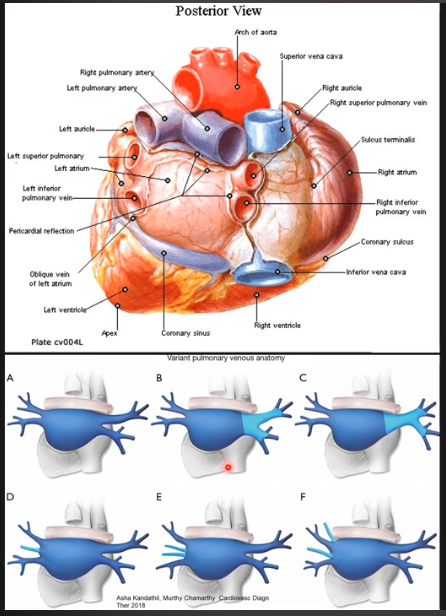
\includegraphics[keepaspectratio]{images/pulmonaryveinanatomy.png}}
\pandocbounded{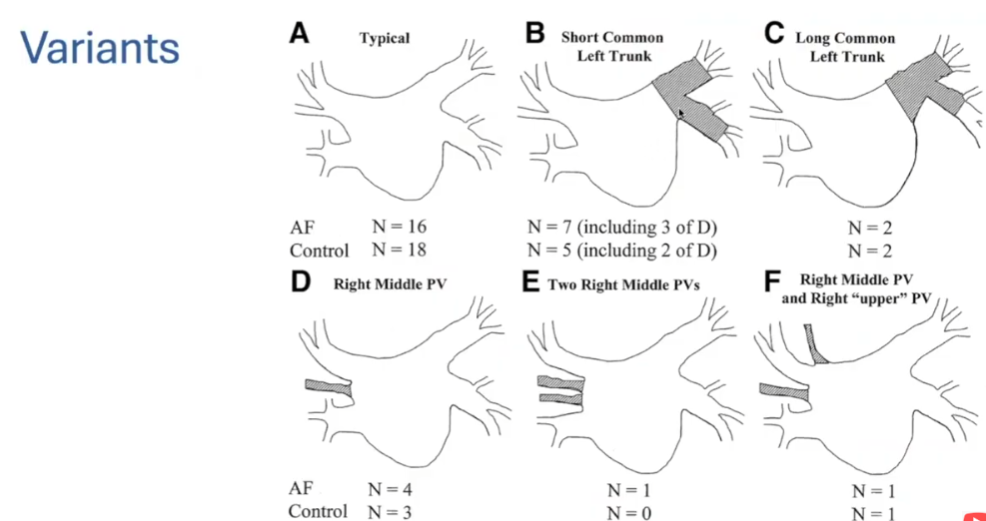
\includegraphics[keepaspectratio]{images/variants.png}}

Keuhkolaskimoiden arvioiminen TTE:ssä on yleensä vaikeaa, mutta usein mahdollista. Jos niiden tarkkaa arvioita tarvittaisiin syystä tai toisesta, niin TEE:llä saadaan paljon kirkkaampi kuva. TTE:llä muiden mittausten yhteydessä arvioidut keuhkolaskimot voivat kuitenkin tarjota usein arvokasta lisädataa.

Yleisesti voi ajatella, että oikeanpuoleiset laskimot näkyvät paremmin (tai ainakin virtaukset ovat paremmin mitattavissa, koska virtaukset ovat enemmän anturin suuntaisia) apikaalisissa projektioissa, kun taas vasemmat laskimot parasternaalisesti. Yleensä siis parhaiten A4C-projektiosta saadaan mitattua RUPV ja se onkin yleisimmin käytetty suoni mittauksissa. Muiden projektioiden ja suonien hyödyntäminen on harvinaisempaa, mutta ne on hyvä oppia tunnistamaan, jottei kuvittele normaalien keuhkolaskimoiden olevan epänormaaleja rakenteita.

\subsection{Apikaalisesti}\label{apikaalisesti}

Oikeat keuhkolaskimot voidaan tunnistaa apikaalisesta kuvasta eteisväliseinän viereisinä rakenteina, joista voi dopplerilla nähdä virtausaaltoja. Yleensä parhaiten visualisoituu RUPV. RLPV:n saa visualisoitua tilttaamalla probea hieman alaspäin tai rotatoimalla vastapäivään. Apikaalisesti ei yleensä saada mitattua virtauksia vasemmista laskimoista, vaikka ne visualisoituisivatkin, koska suonet kulkevat yleensä kohtisuorasti anturiin nähden.

Kannattaa yleensä myös säätää Nyquistin rajaa hieman alaspäin, koska virtausnopeudet ovat yleensä hieman hitaammat kuin muualla sydämessä. Jos virtauksia ei siis tule esiin tyypillisellä rajalla, niin voi hitaasti laskea rajaa - yleensä n.~40cm/s tai alle on hyvä.

RUPV on yleensä hieman lähempänä eteisväliseinää ja kulkee sen myötäisenä jatkeena, kun taas RLPV ihan hieman enemmän siitä sivussa ja suoremmin (kts. alla mustavalkoiset kuvat)

\pandocbounded{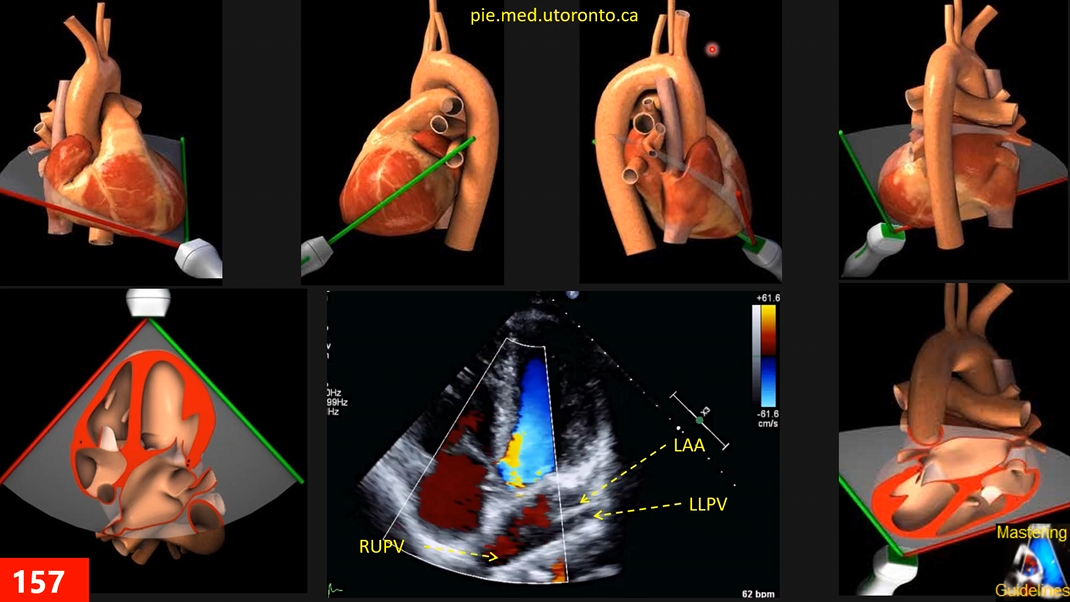
\includegraphics[keepaspectratio]{images/a4crupv.png}}
\pandocbounded{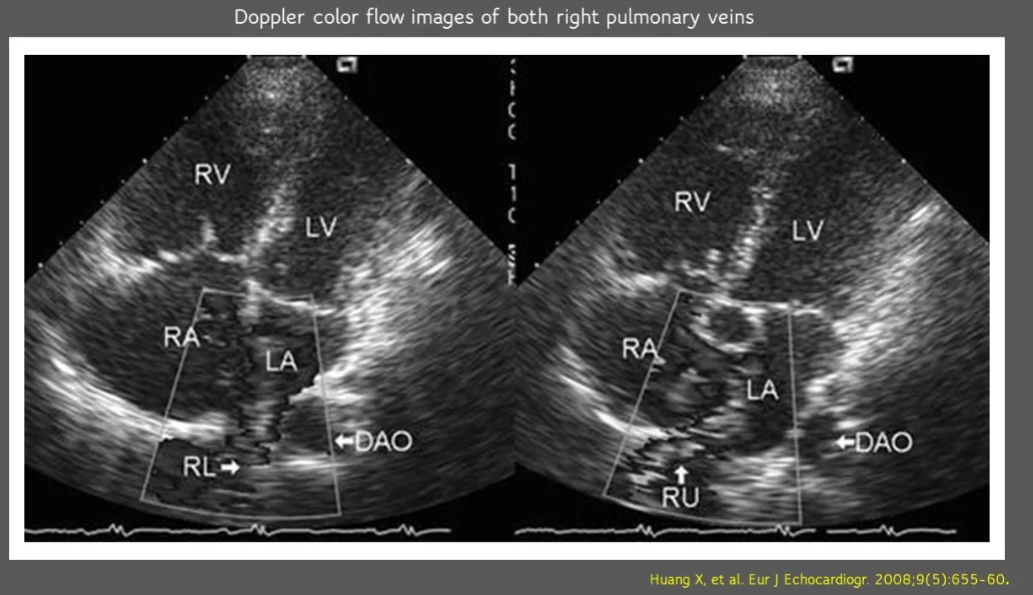
\includegraphics[keepaspectratio]{images/rightpvs.png}}
\pandocbounded{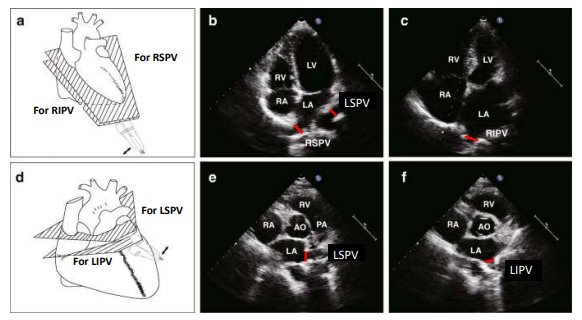
\includegraphics[keepaspectratio]{images/pulmonaryveintte.png}}

\subsection{Parasternaalisesti}\label{parasternaalisesti}

Parasternaalinen keuhkolaskimoiden arvio on harvinaisempaa, mutta mahdollista. Parhaiten voidaan mitata vasempien laskimoiden virtausta ja ne näkyvät PLAX-ikkunassa yleensä laskevan aortan vasemmalla puolella.

\pandocbounded{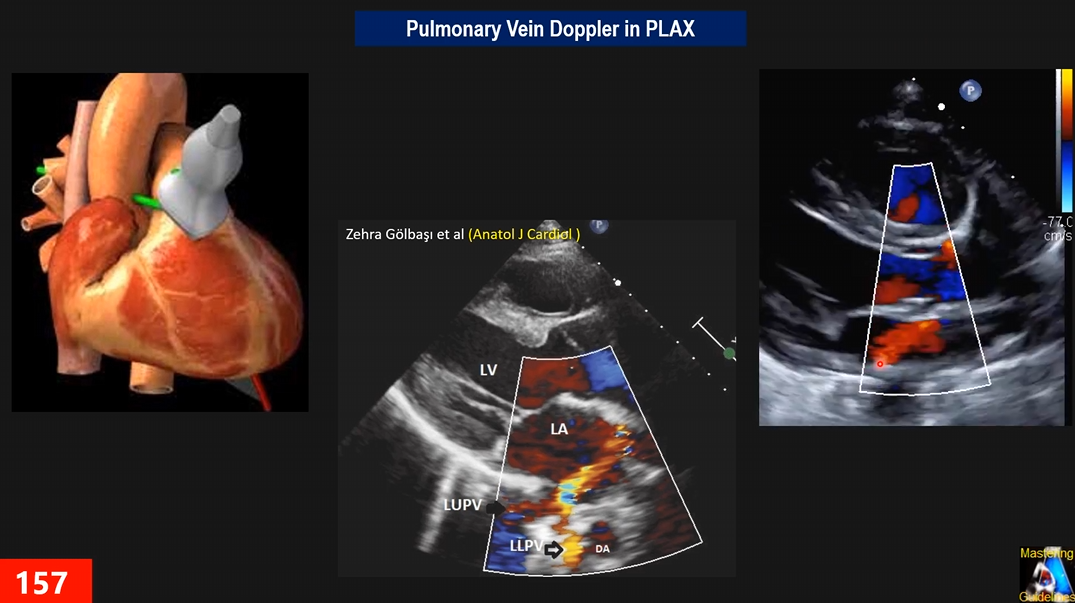
\includegraphics[keepaspectratio]{images/plaxpv.png}}
\pandocbounded{\includegraphics[keepaspectratio]{images/plaxpvvideo.gif}}

PSAX-ikkunassa taas on usein ongelmana se, että laskimo kulkee kohtisuorasti anturiin eikä doppleria saa luotettavasti mitattua. Tämä ongelma on kuitenkin yleensä pääasiassa LUPV:n kanssa ja LLPV saadaan visualisoitua, kun hieman siirretään anturia potilaan päätä kohti ja tiltataan alaspäin. Tällöin LLPV visualisoituu LUPV:n alle enemmän anturinsuuntaisesti kulkevana suonena, josta saa dopplerilla virtaukset hyvin esiin. RUPV myös usein visualisoituu samalla.

\pandocbounded{\includegraphics[keepaspectratio]{images/pvpsax.gif}}

\chapter{Vasen kammio}\label{vasen-kammio}

Ultratessa tulee usein unohdettua, että sydän on kompleksi kolmiulotteinen rakenne. 2D-echoa tuijottaessa nähdään vain liike tietyllä leiketasolla eikä pystytä arvostamaan sydämen oikeaa liikettä, joka on esim. vasemman kammion kannalta niin pitkittäissuuntaista kuin kiertävää. Onkin siis tärkeää muistaa, että yksittäinen mittaus yksittäiseltä leiketasolta ei kerro koko tarinaa, varsinkaan vasemman kammion toimintaa arvioitaessa. Tämän takia kannattaa harjoitella arvioimaan sydäntä monesta eri näkökulmasta ja keräämään tuloksia moniparametrisesti - täten saa tarkemman ja luotettavamman arvion mistä tahansa rakenteesta, jota tutkii.

\pandocbounded{\includegraphics[keepaspectratio]{images/sydäntorsio.gif}}

\section{Vasemman kammion mitat}\label{vasemman-kammion-mitat}

Vasemman kammion mitat kerätään useimmiten PLAX-projektiosta ja tyypillisesti lisäksi myös vähintään apikaalisesti.

Tyypillisimmät mitattavat arvot ovat seinämien paksuudet sekä ejektiofraktion laskemiseksi diastolinen ja systolinen läpimitta (ja apikaalisesti tilavuuden arvio piirtämällä).

\subsection{PLAX}\label{plax}

Parasternaalinen pitkittäisakseli on tyypillisellä potilaalla yleensä ensimmäiseksi haettu projektio ja se on myös yleisimmin käytetty projektio vasenta kammiota mitattaessa. Tavoitteena on saada sydän kuvaan niin, että kammio ei ole lyhennetty (forshortened). Kammion ei tulisi näyttää apeksistaan pyöreältä (johtuu siitä, että ultraäänellä ei leikata oikeaa kärkeä). Yleensä forshorteningin siis tunnistaa siitä, että apeksi ``työntyy'' kammioon ja kammio näyttää pieneltä pussilta. Apeksia ei edes tulisi näkyä oikein suunnatussa PLAX-projektiossa. Yleensä paras troubleshooting-vinkki on rotatoida anturia hieman myötäpäivään - tämä auttaa kammion ``avaamisessa''. Joskus tarvitsee siirtää anturia yksi kylkiluuväli alaspäin ja joskus tarvitsee tehdä tilttausliikkeitä.

\pandocbounded{\includegraphics[keepaspectratio]{images/plaxforshortening.gif}}
\pandocbounded{\includegraphics[keepaspectratio]{images/plaxonaxis.gif}}

\subsubsection{Mittaustekniikat ja yleinen ongelma}\label{mittaustekniikat-ja-yleinen-ongelma}

Kammion ulottuvuudet voidaan mitata niin suoraan B-kuvasta kuin M-moodikäyrästä. M-moodilla voidaan saada hyvinkin tarkat ja nopeat mittaukset, mutta sen ongelmana on yleensä mm. sydämen ``väärä'' asento ja/tai heikkotasoinen kuva. Myös pienten kammioiden ``pseudoshortening'' papillaarilihasten tullessa mittausviivalle on suhteellisen yleinen ongelma.

\textbf{Tärkeä periaate: sydänrakenteiden ulottuvuuksien mittaus tulisi tapahtua kohtisuorasti niiden pitkittäisakseliin nähden.}

M-moodissa leikkauslinja tulisi asettaa siten, että se katkaisee kohtisuorasti vasemman kammion heti mitraaliläpän avautuvien purjeiden kärkien distaalipuolelta. Jos sydämen asento on liian pysty (todella usein on), niin M-moodi katkaisee kammion liian vinosti. Tämä mm. yliarvioi vasemman kammion poikkimittaa. Jos ei saa kunnollista kohtisuoraa leikettä, niin voi periaatteessa vääntää itse leikkauslinjan kulmaa, mutta se usein tekee kuvasta liian ``pehmeän'' ja vaikeatulkintaisen. Suosittelenkin, että jos ei saa kunnollista kohtisuoraa leikettä tai tarpeeksi hyvälaatuista kuvaa, niin kannattaa mittaukset tehdä suoraan B-kuvasta (usein muutenkin kannattaa tehdä ns. laatukontrollina, vaikka saisikin M-moodilla mitattua). Nykysuosituksissa (ASE) B-kuvasta piirtämistä pidetään yleisestikin parempana kuin M-moodia. B-kuvamittauksissa voi suunnata mittauslinjat rakennespesifisesti ja täten saada luotettavampia arvoja - ei siis tarvitse mitata suoraan samasta linjasta kaikkia vasemman kammion mittoja, vaan esimerkiksi seinämät ja läpimitan voi piirtää erisuuntaisilla viivoilla riippuen niiden pitkittäisakselista; seinämät ja kammiolokero eivät siis aina kulje samassa linjassa.

Alla olevassa kuvassa vain keltainen linja kulkee kohtisuorasti vasemman kammion pitkittäisakseliin nähden. Vaalea ja punainen linja leikkaavat kammion liian pystysuorasti eikä niitä voi siten pitää luotettavina mittauksina. M-moodilinja lähtee normaalisti siis UÄ-kartion huipulta eli normaalisti saisi vain punaisen tai vaalean linjan kautta tehtyä mittauksia. Jos kuitenkin aivan pakottavasti haluaa tehdä M-moodista mittaukset, niin mittauslinjan voi vääntää keltaisen suuntaiseksi, mutta yllä mainitun mukaisesti se tekee M-moodin kuvanlaadusta yleensä liian huonon luotettavaa tulkintaa varten.

\pandocbounded{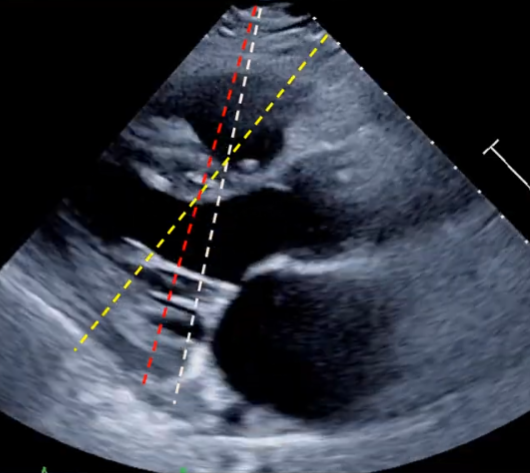
\includegraphics[keepaspectratio]{images/mmodelineslv.png}}

\pandocbounded{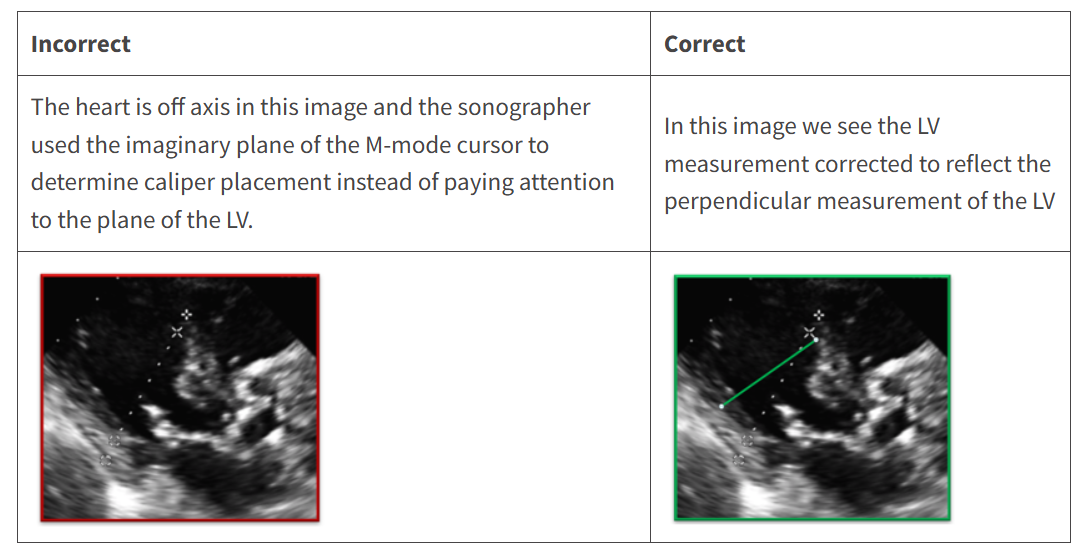
\includegraphics[keepaspectratio]{images/offaxislv.png}}
\pandocbounded{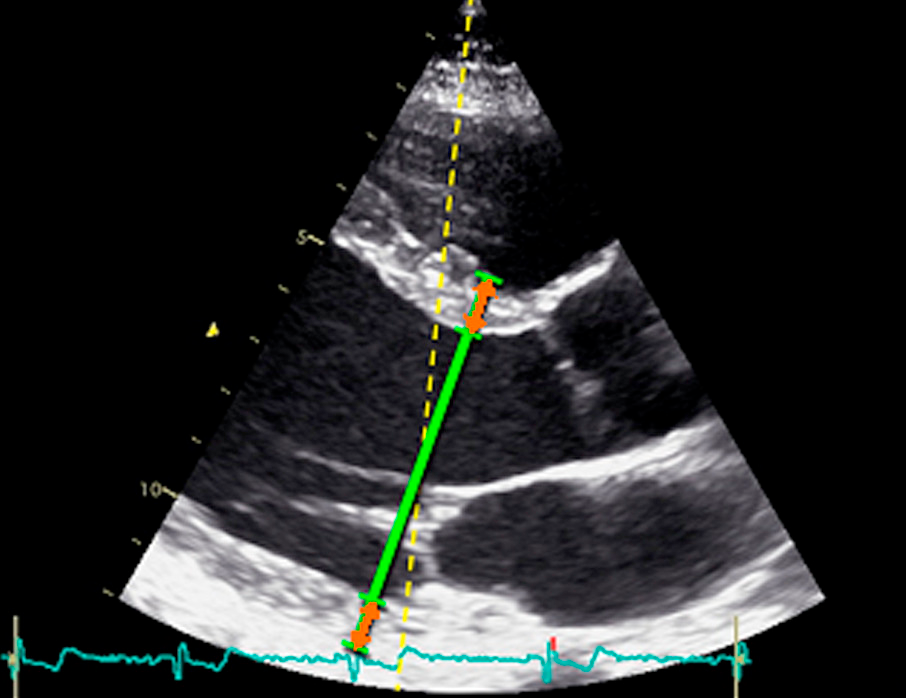
\includegraphics[keepaspectratio]{images/2dvsmm.png}}

\subsubsection{Mitattavat suureet ja aloittaminen}\label{mitattavat-suureet-ja-aloittaminen}

Aluksi siis haetaan mahdollisimman hyvä projektio, jonka jälkeen kuva pysäytetään painamalla UKG-laitteen nappulaa \textbf{``Freeze''.} Sitten pallohiireä liikuttamalla saa siirrettyä pysäytystä edeltävää talletetta ajassa taaksepäin (ja eteenpäin).

PLAX-kuvasta yleensä mitataan vähintään seinämien paksuudet (diastolessa) sekä läpimitta diastolessa ja systolessa. Sydämen tarkkaa sähköisen syklin vaihetta ei tarvitse miettiä, vaan pysäytetystä kuvasta haetaan vain loppudiastole ja loppusystole visuaalisin perustein: loppudiastole on silloin, kun LV:n läpimitta on suurimmillaan ja loppusystole LV:n ollessa pienimmillään.

Kun on löytänyt loppudiastolen eli sen hetken, jossa vasen kammio on suurimmillaan, niin voi aloittaa mittaamisen.

\paragraph{IVS:n mittaus}\label{ivsn-mittaus}

Yleensä mittaukset aloitetaan kammioväliseinämästä (interventricular septum, IVS) ja siirrytään siitä alaspäin - oikean kammion mittauksia ei lähes koskaan suoriteta tästä näkymästä. Valitaan siis Calc-nappulan takaa Main Menu --\textgreater{} Dimensions --\textgreater{} IVSd (MM). Kun kertoo koneelle, että mittaa väliseinämää, niin se siirtyy tämän jälkeen automaattisesti seuraaviin mittoihin eli läpimittaan ja sen jälkeen vielä takaseinämään.

Mittaa IVS esimerkkikuvan mukaisesti lihaksensisäisesti (älä siis laita crosshairia mustaan vereen, vaan juuri lihaksen uloimpaan kohtaan).

\pandocbounded{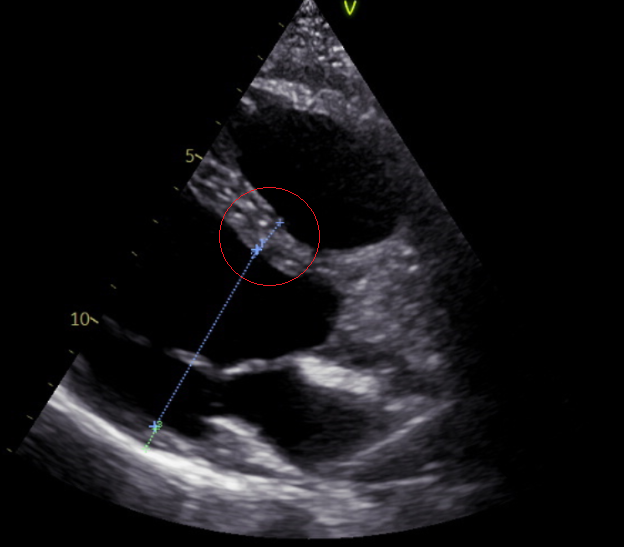
\includegraphics[keepaspectratio]{images/ivsmeasurement.png}}

\paragraph{LV:n mittaus (diastole)}\label{lvn-mittaus-diastole}

Jos mittasit edellä IVS:n, UKG-laite siirtyy suoraan vasemman kammion diastolisen mitan (LVIDd, left ventricular internal dimension in diastole) kohdalle. Joskus septumin mittausta ei voi oikein luotettavasti suorittaa sen demarkoituessa huonosti, jolloin voi valita Calc-nappulan takaa suoraan Main Menu --\textgreater{} Dimensions --\textgreater{} LVIDd (MM), ja jättää IVSd:n (ja RVIDd:n) tässä yhteydessä mittaamatta.

Mittaa LVIDd alla olevan esimerkkikuvan mukaisesti kudoksesta kudokseen eli inner edge to inner edge (ei siis verestä vereen). Mittaus tulisi tyypillisesti aloittaa suoraan IVS:n kammionpuoleisesta mittauspisteestä.

\pandocbounded{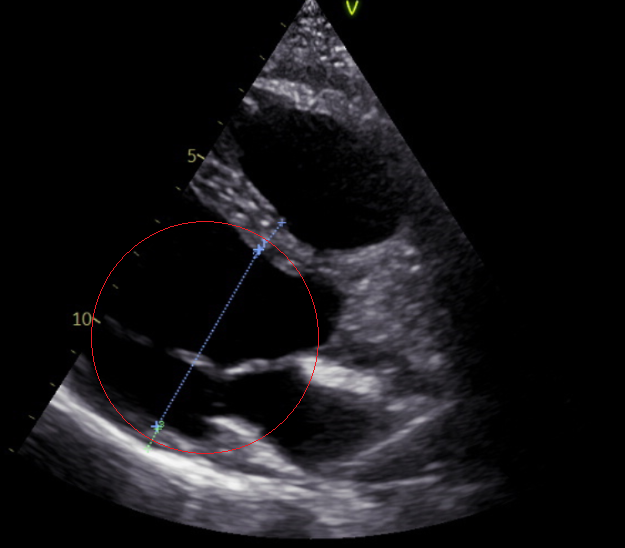
\includegraphics[keepaspectratio]{images/lviddmeasurement.png}}

\paragraph{LVPW:n mittaus}\label{lvpwn-mittaus}

Jos mittasit edellä LVIDd:n, UKG-laite siirtyy suoraan vasemman kammion takaseinän (LVPWd) kohdalle. Mittaa LVPWd alla olevan esimerkkikuvan mukaisesti lihaksen kammiopuolisesta osasta perikardiumiin. Mittaus tulisi tyypillisesti aloittaa suoraan LVIDd:n mittauksen loppupisteestä.

\pandocbounded{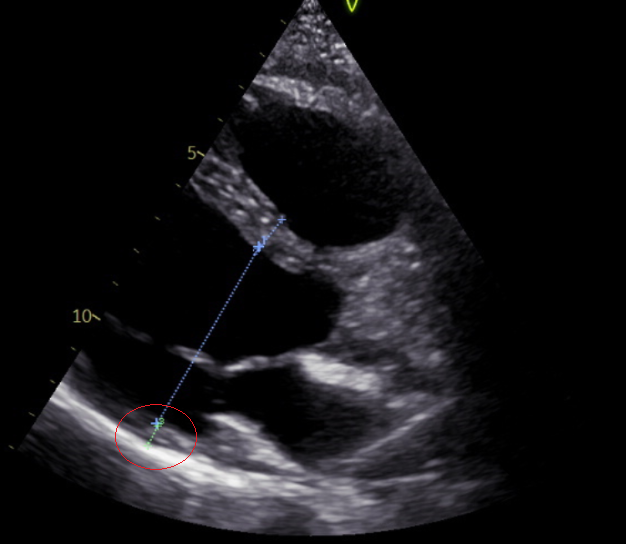
\includegraphics[keepaspectratio]{images/lvpwmeasurement.png}}

\paragraph{LV:n mittaus (systole)}\label{lvn-mittaus-systole}

B-kuvasta piirtäen tulee tässä kohtaa useilla koneilla poistua calc-ikkunasta, jotta pääsee taas pyörittämään sydänsykliä eteen-/taaksepäin (jos olisi M-moodissa, niin LVPWd:n mittauksen jälkeen kone ehdottaisi suoraan LVIDs:ää (left ventricular internal dimension in systole) ja voisi mitata sen heti samalta näytöltä). Seuraavaksi siis tulee mitata vasemman kammion läpimitta loppusystolessa eli etsitään kuva, jossa vasen kammio on pienimmillään. Mittaus tulisi suorittaa samasta sydänsyklistä kuin mistä diastolinen läpimitta oltiin otettu.

Kun on löytänyt sen hetken, kun vasen kammio on pienimmillään, niin voi mitata sen läpimitan esimerkkikuvan mukaisesti (taas calcin kautta tietysti). Systolessa ei enää yleensä mitata seinämien paksuuksia; joskus nekin voidaan kyllä mitata kvantitatiivisen paikallisen ja globaalinen kontraktiliteetin lisäarviona, mutta useimmiten tätä ei tarvita.

\pandocbounded{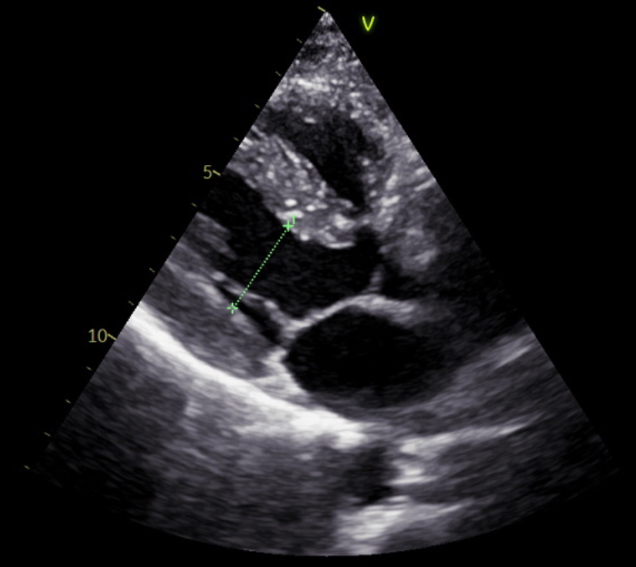
\includegraphics[keepaspectratio]{images/lvidsmeasurement.png}}

Jos oli aikaisemmin mitannut LVIDd:n niin LVIDs:n saatuaan kone laskee ja ilmaisee ``jakoviivan'' alla keskeisiä laskennallisia suureita, joista yleensä ilmoitetaan lausunnossa vain fraktionaalisen lyhentymän kautta (fractional shortening eli FS\% = (LVIDd-LVIDs)/LVIDd x 100) Teichholzin metodilla laskettu ejektiofraktio (EF). Seinämäpaksuudet ilmoitetaan lausunnossa myös, jos ne on saatu mitattua. Alla olevasta kuvasta voisi siis kirjoittaa lausuntoon: ``LV 40/23, josta EF 75 \%. Seinämät 11/14.''

Tulokset siis ilmaistaan millimetreissä eikä yksikköä (mm) yleensä merkata. LV 40/23 tarkoittaa vasemman kammion läpimittaa diastolessa / systolessa ja tästä lasketaan ejektiofraktio (EF). Seinämät ilmoitetaan järjestyksessä kammioväliseinä / takaseinä.

Normaali ejektiofraktio on välillä 50-70\%.

HFmrEF (heart failure with mildly reduced ejection fraction) on välillä 41-49\%

HFrEF (heart failure with reduced ejection fraction) on 40\% tai alle

LV on ``hyperdynaaminen'' jos EF on yli 70\%

Tämä ei sinänsä ole yleensä levossa hyvä asia ja viittaa taustalla olevaan patologiaan (esim. läppävuodot, high-output-tilat (anemia, hypertyreoosi), hypovolemia\ldots)

Mielenkiintoisesti ``optimaalinen'' EF kuolleisuuden kannalta on \href{https://pmc.ncbi.nlm.nih.gov/articles/PMC8204658/}{tutkimusten} mukaan 60-65\% ja tämän ulkopuolella kuolleisuus on EF:n suhteen U-käyrämäinen

Joskus myös ilmoitetaan LV:n massa ja jos ilmoitetaan niin yleensä indeksoituna kehon pinta-alaan (BSA). LV:n massaa ilmoitetaan aika harvoin lausunnoissa, mutta periaatteessa se on yksi vasemman kammion hypertrofian mittareista; yleensä kuitenkin vain seinämäpaksuudet riittää lausunnossa.

Kannattaa huomioida, että tämä ejektiofraktio ei ole täydellinen arvio. Teichholzin metodi siis perustuu siihen, että vasemman kammion ajatellaan olevan täydellinen sylinteri ja kammion läpimitan fraktionaalisen lyhentymän perusteella voidaan päätellä koko sylinterin tilavuuden ejektiofraktio. Vasen kammion ei kuitenkaan ole sylinteri ja täten ejektiofraktion arvio ei ole täydellinen. Tarkempi arvio saadaan Simpsonin metodilla (tästä enemmän hieman alempana), mutta parasta on kerätä useita ejektiofraktioarvioita ja ottaa ne kaikki huomioon lopullisessa päättelyssä.

\pandocbounded{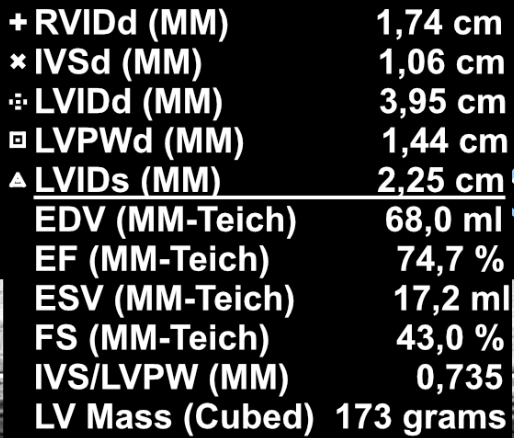
\includegraphics[keepaspectratio]{images/tuloksialv.png}}

\paragraph{Sama M-moodilla}\label{sama-m-moodilla}

Jos saa poikkeuksellisen hyvän leikkaussuunnan M-moodia varten, niin mittaukset kyllä voi ihan hyvillä mielin tehdä M-moodistakin. Mittaukset tehdään samalla periaatteella kuten yllä. Huomioi esimerkkikuvasta, että systolisia seinämäpaksuuksia ei yleensä tarvitse mitata.

M-moodi kuva siis saatiin asettamalla leikkauslinja heti mitraaliläpän avautuvien purjeiden kärkien distaalipuolelle kohtisuorasti kammion pitkään akseliin nähden. Sitten voi painaa koneesta M-mode ja jos tuotettu M-moodikäyrä näyttää hyvältä, niin voi painaa Freeze ja tehdä mittaukset Calc:n kautta avautuvasta valikoista (Main Menu -\textgreater{} Dimensions -\textgreater{} IVSd (ja sen jälkeen kone tarjoaakin automaattisesti LVIDd, LVPWd ja LVIDs järjestyksessä)).

\pandocbounded{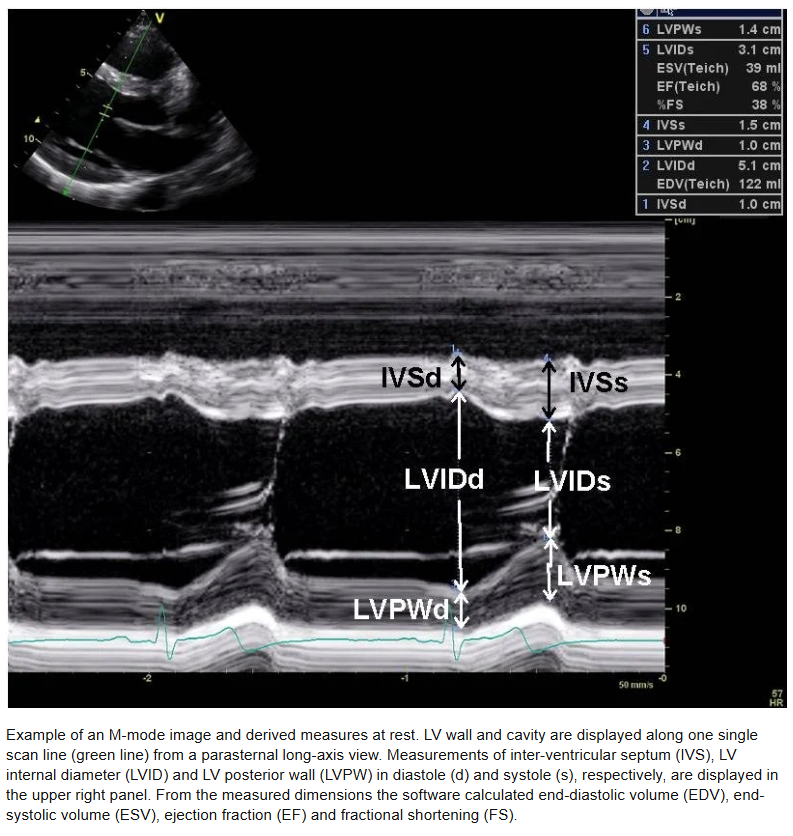
\includegraphics[keepaspectratio]{images/mmodelv.png}}

M-moodi (motion mode) siis tarkoitti ultraääänitekniikkaa, jossa arvioidaan vain yhden ohuen sydämen linjan liikettä ajan funktiona - käyrässä siis aika on x-akselilla. Käyrän y-akseli muodostuu leikkauslinjan rakenteista ja niiden liikkeestä. On hyvä tunnistaa B-kuvasta rakenteet ja arvioida ne visuaalisesti ensin tarkasti ja vasta sen jälkeen painaa M-mode päälle, jotta osaa tunnistaa M-käyrältä rakenteet ja miten ne suhteutuvat B-kuvaan.

\pandocbounded{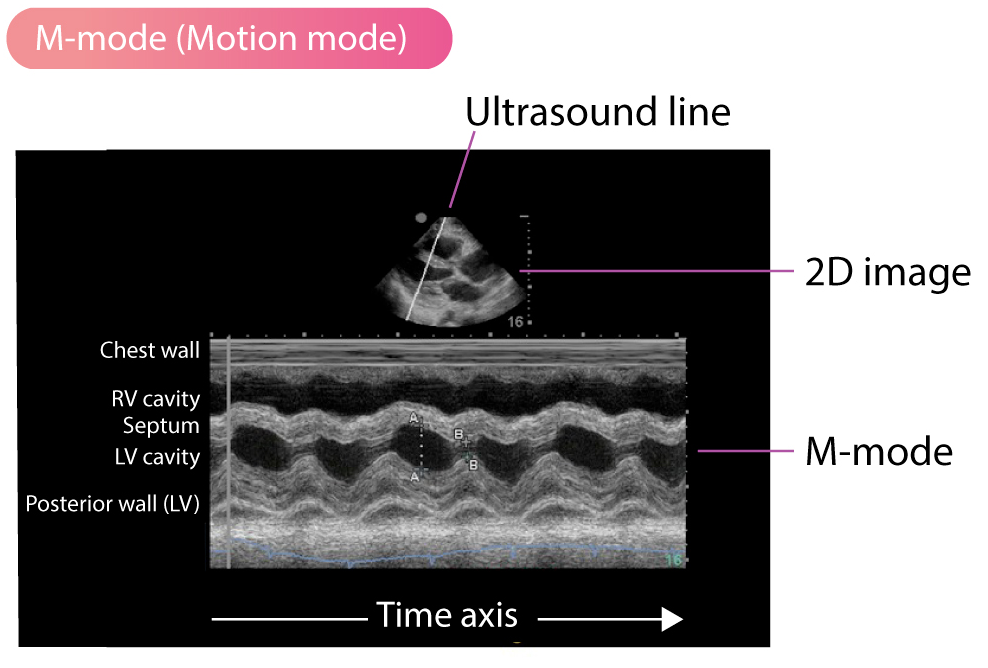
\includegraphics[keepaspectratio]{images/mmodelvexplained.png}}

\subsection{Apikaalisesti}\label{apikaalisesti-1}

Vasemman kammion mittoja kannattaa aina mahdollisuuksien mukaan kerätä PLAX:n lisäksi myös apikaalisista projektioista. Tyypillisimmin mitattavat arvot ovat kammion loppudiastolinen tilavuus (LVEDD) ja loppusystolinen tilavuus (LVESD). Näistäkin kone pystyy tietysti laskemaan ejektiofraktion.

Mittauksissa hyödynnetään Simpsonin metodia, jossa tilavuus integroidaan kuvittelemalla kammio kooltaan eroaviksi kiekoiksi. Kammion pinta-ala siis planimetroidaan tyypillisesti apikaalisesta nelilokerokuvasta ja tällä tavalla saadaan kiekkopatsaan korkeus ja leveys eri tasoilla. Mittauksessa on geometrinen oletus, että kammion poikkileikkaus on ympyränmuotoinen jokaisella tasolla. Kammio ei kuitenkaan tällainen ole, joten paremman arvion saa, kun hakee vielä apikaalisen kaksilokerokuvan ja tekee mittaukset siitäkin. Tällä tavalla saa kaksi läpimittaa kohtisuorista kuvakulmista ja siten luotettavamman keskiarvon - tätä kutsutaan Simpson's Biplane -metodiksi.

\pandocbounded{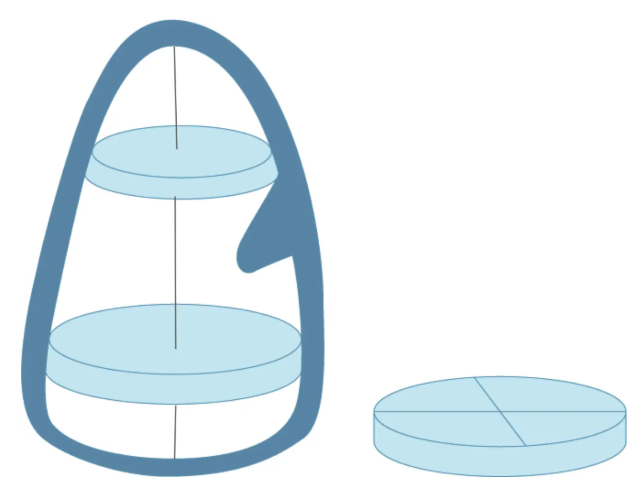
\includegraphics[keepaspectratio]{images/simpsonmethod.png}}
\pandocbounded{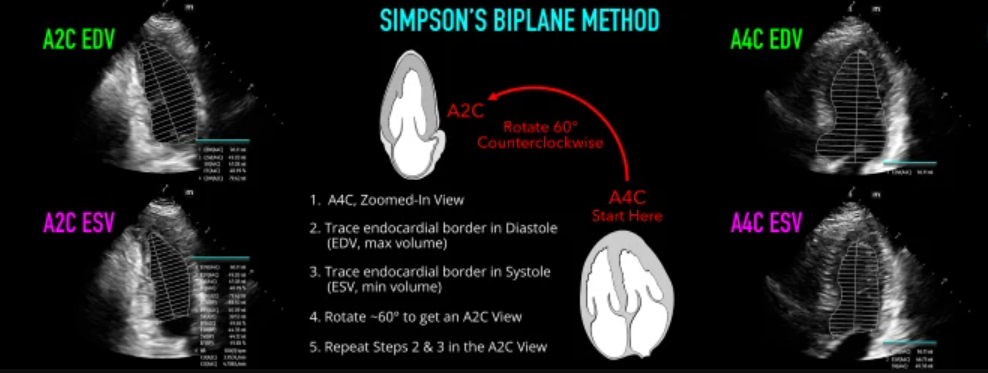
\includegraphics[keepaspectratio]{images/simpsonbiplane.png}}

\subsubsection{Taas muistutus lyhentymisestä}\label{Muistutus}

Vaikka Simpson's Biplane -metodi on tällä hetkellä tarkin 2D-ekokardiografinen LVEF:n mittaustapa, niin se on myös todella käyttäjäriippuvainen. Yksi yleisimmistä virhelähteistä on taas forshortening eli lyhentymä, jossa sydäntä ei leikata ultraääniaalloilla sen oikeasta apeksista, jolloin ei saada mitattua kammion oikeita mittoja. Tämän takia kammion tilavuudet ovat ultraäänellä mitattuina yleensä pienempiä kuin sydämen MRI:ssä saadut arvot. Lyhentymän takia myös mm. apikaaliset trombit voivat jäädä havaitsematta.

Lyhentymän voi tunnistaa monista piirteistä:

Lyhentymässä vasen kammio on pussimainen eikä tyypilliseen tapaan ``luodinmuotoinen''

False apex on yleensä myös seinämältään paksumpi kuin sen pitäisi olla

Papillaarilihasten sijainti: papillaarilihaksia ei tulisi nähdä apikaalisimmassa kammion kolmanneksessa

Apeksin liikehdintää on myös tärkeää arvioida: Kammion kärki ei supistu ja liiku sisäänpäin kammioon, vaan sen tulisi supistua oman keskipisteensä ympärille (apeksin tulisi siis olla samassa paikassa niin diastolessa ja systolessa); jos apeksi ``työntyy'' kammioon, niin löydös on joko patologinen tai yleensä lyhentymästä johtuvaa

\pandocbounded{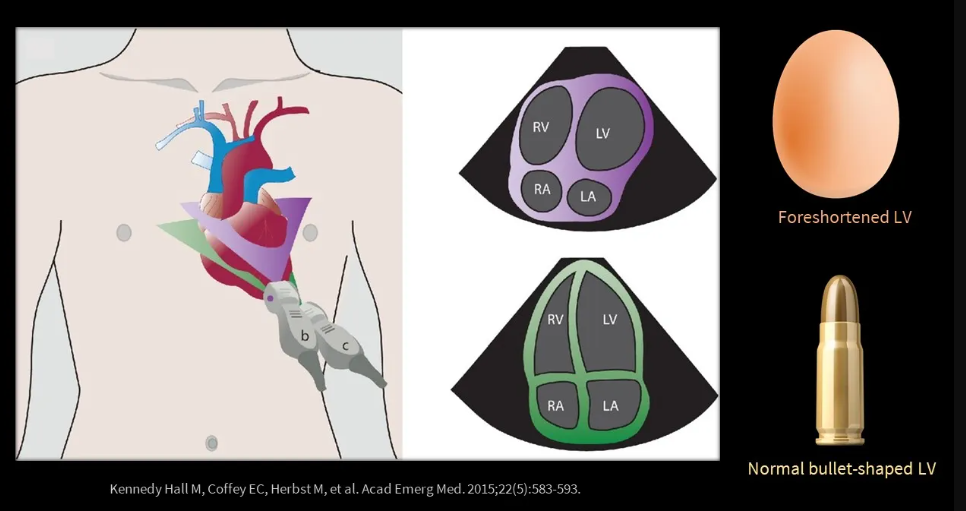
\includegraphics[keepaspectratio]{images/a4cforshortening.png}}
\pandocbounded{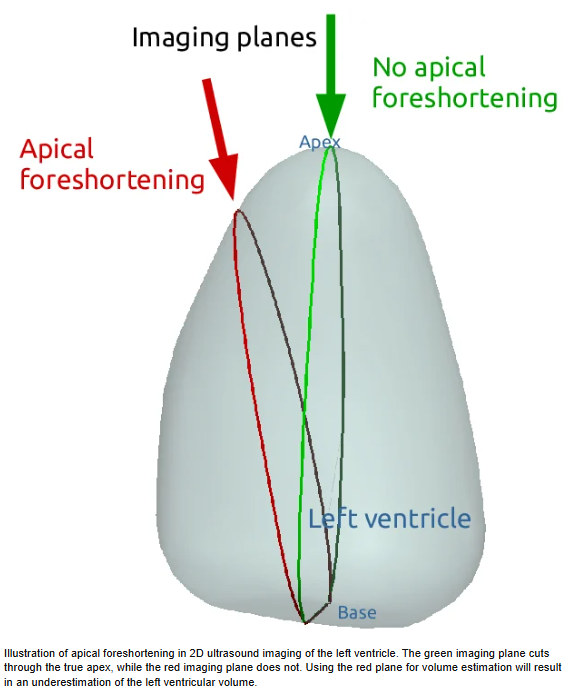
\includegraphics[keepaspectratio]{images/falseapex.png}}
\pandocbounded{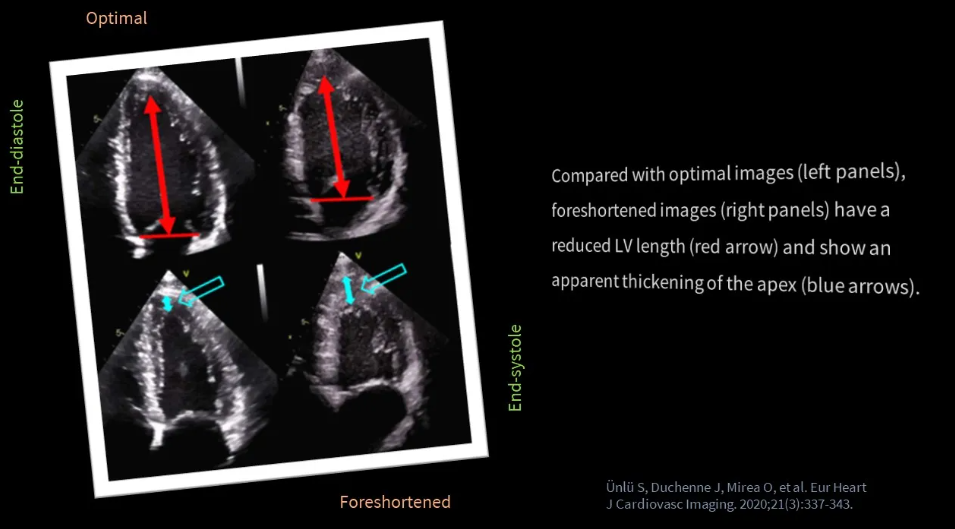
\includegraphics[keepaspectratio]{images/a4cforshortening2.png}}

Tässä videossa näkyy papillaarilihas apikaalisimmassa kolmanneksessa ja myös kärjen supistumista kammion sisälle. False apex on myös optimaaliseen kuvaan verrattuna paksumpi ja pyöreämpi.

\pandocbounded{\includegraphics[keepaspectratio]{images/forshorteninga4c.gif}}

\subsubsection{LVEDD}\label{lvedd}

Mittaukset kannattaa aloittaa apikaalisesta nelilokerokuvasta ja vasta sen jälkeen arviota tarkentaessaan siirtyä kaksilokerokuvaan (sitä ei aina tarvita, mutta on hyvä jos ehtii ottamaan). Tarkoitus on siis ensiksi löytää oikeaoppinen projektio, jonka jälkeen jäädyttää kuva ja kelata syklejä takaisin niin, että löytää sen hetken, jolloin kammio on isoimmillaan (end-diastolic volume, LVEDD). Sitten voi calc:n kautta hakea LVEDD:n ja piirtää kammion sisäpinta-alan eli tulee seurata endokardiumin rajoja. Endokardiumin rajojen tarkka näkeminen on usein todella vaikeaa ja joskus mahdotonta eikä sydämen sisäpinta ole millään mittarilla sileä - se on täynnä häiritseviä rakenteita, kuten papillaarilihaksia, chordia ja trabekulaatioita.

Endokardiumin piirtämiseen muutamia vinkkejä:

Kannattaa ``treenata'' silmää endokardiumin rajoille liikuttelemalla sykliä eteen- ja taaksepäin ja aloittaa mittaus vasta kun on saanut tätä kautta käsityksen rajoista - pelkästä paikallaan olevasta kuvasta on vaikeaa tunnistaa rajoja tarkasti

Mittaus aloitetaan mitraaliannuluksesta ja viedään toisen puolen annulukseen; yleensä lateraalinen -\textgreater{} mediaalinen suunta eli myötäpäivään; jos kuva olisi viisilokerokuva, niin LVOT:n avautuminen yleensä häiritsee mediaalipuolen arviointia, jonka takia mittaukset tehdään ilman aortan visualisaatiota

Älä ota papillaarilihaksia tai trabekulaatioita huomioon piirtäessä

Kammion pitkittäisakselin ja annulustason leveys tulisi optimaalisesti olla kohtisuorasti, muuten voi jäädä tilaa laskelmien ulkopuolelle

\pandocbounded{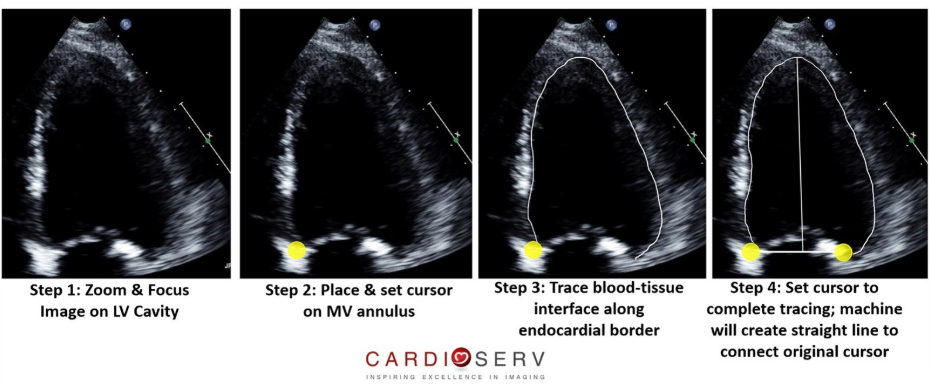
\includegraphics[keepaspectratio]{images/tracingapical.png}}
\pandocbounded{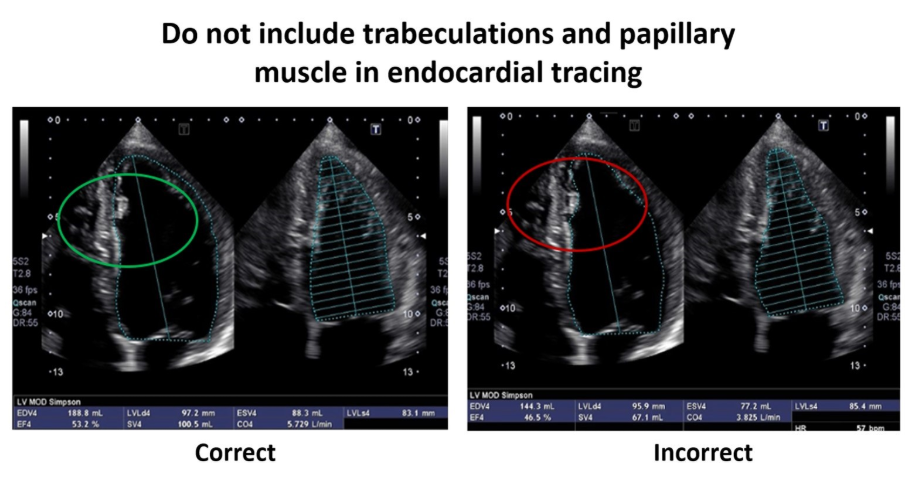
\includegraphics[keepaspectratio]{images/donotinclude.png}}
\pandocbounded{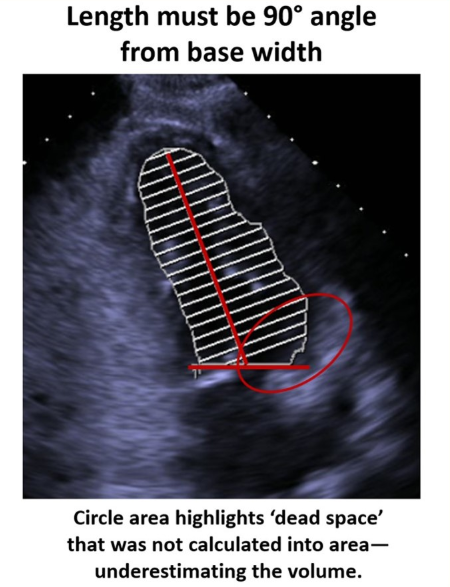
\includegraphics[keepaspectratio]{images/apexperpendicular.png}}

\subsubsection{LVESD}\label{lvesd}

Seuraavaksi poistetaan diastolinen mittaus näytöltä ja kelataan loppusystoleen eli siihen kohtaan sykliä, jossa vasen kammio on pienimmillään. Sitten piirretään taas sisäpinta. Tämän jälkeen kone laskee ejektiofraktion.

Sitten vielä tehdään samat apikaalisesta kaksilokerokuvasta (A2C).

\pandocbounded{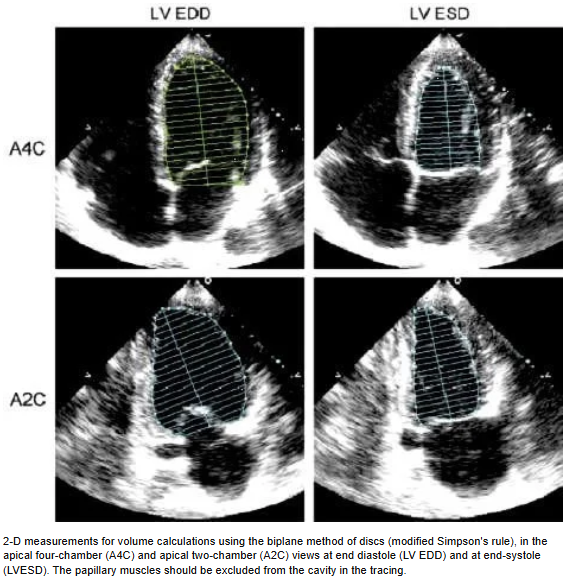
\includegraphics[keepaspectratio]{images/lvesd.png}}

\subsection{PSAX}\label{psax}

Myös parasternaalisesta poikittaiskuvasta voi mitata vasemman kammion mittoja ja ejektiofraktion. Projektiosta voi myös mitata vasemman kammion massan (LV Mass) hieman eri tavalla kuin miten se lasketaan PLAX-kuvasta (kone siis laskee LV:n massan, jos on mitattu IVSd, LVIDd ja LVPWd). LV:n massaa ilmoitetaan aika harvoin lausunnoissa, mutta se periaatteessa on yksi vasemman kammion hypertrofian mittareista; yleensä kuitenkin vain seinämäpaksuudet riittää lausunnossa.

\subsubsection{PSAX-ejektiofraktio}\label{psax-ejektiofraktio}

Ejektiofraktiota arvioitaessa PSAX-projektiosta, tulisi kuvata papillaarilihasten tasoa.

\pandocbounded{\includegraphics[keepaspectratio]{images/psaxlevel.gif}}

Seuraavaksi seinämät ja läpimitta (läpimitta diastolessa ja systolessa) mitataan joko B-kuvasta tai M-moodista esimerkkikuvan mukaisesti:

\pandocbounded{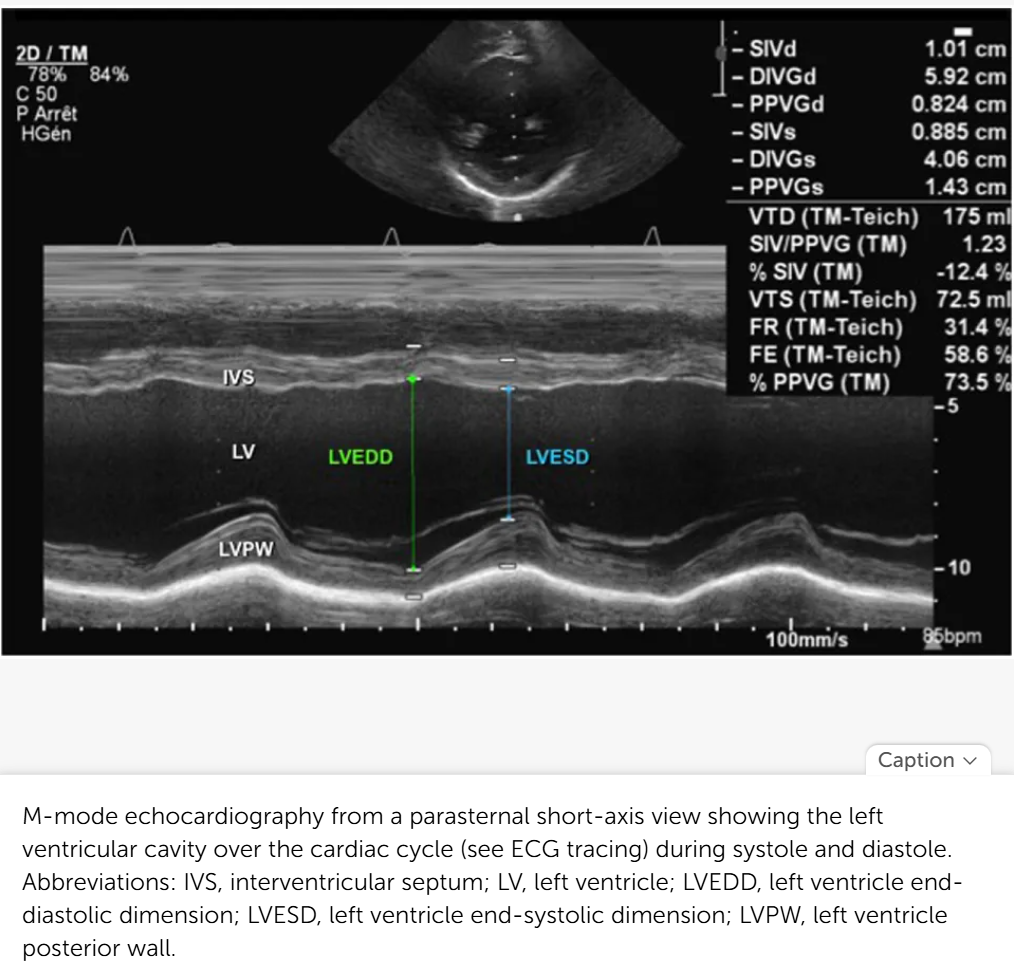
\includegraphics[keepaspectratio]{images/psaxmmode.png}}

Voi myös laskea ejektiofraktion ns. fraktionaalisen pinta-alan muutoksen kautta planimetroiden papillaarilihastason sisäpinta-alan:

\pandocbounded{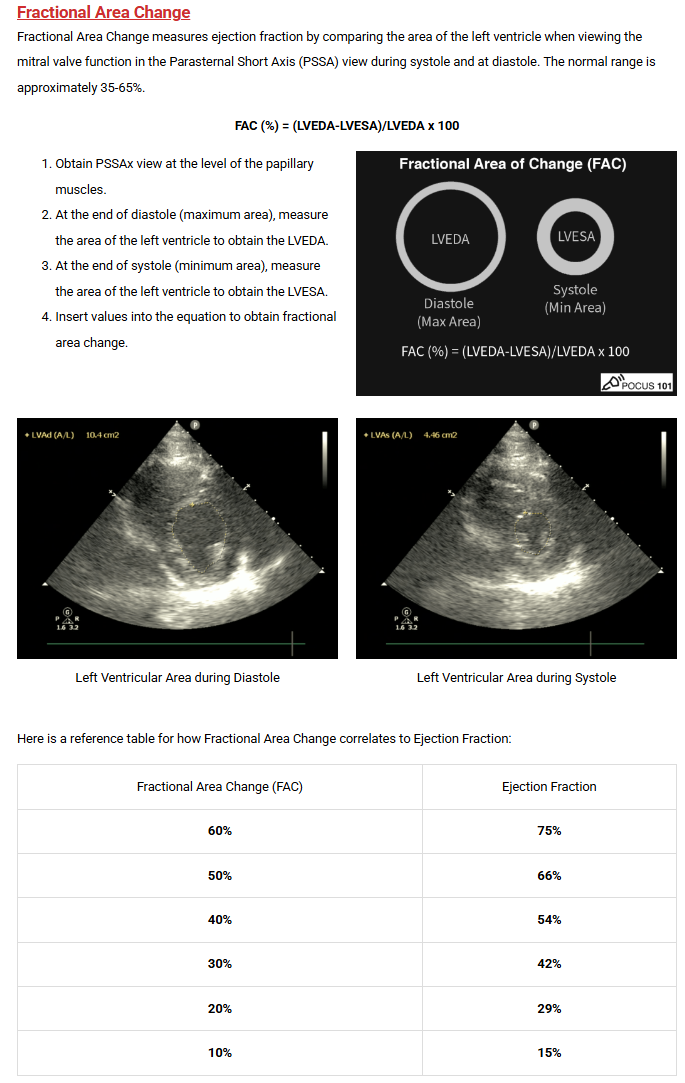
\includegraphics[keepaspectratio]{images/fac.png}}

\section{Silmämääräinen arvio}\label{Silmamaarainen-arvio}

Tutkimuksien (\href{https://pubmed.ncbi.nlm.nih.gov/15882665/}{esim. Gudmundsson et al., 2005}) mukaan \textbf{silmämääräinen ejektiofraktion arvio korreloi todella tarkasti kvantitatiivisten mittausten kanssa - se voi jopa olla tarkin ekokardiografinen metodi LV:n systolisen funktion arvioimisessa.} Joskus huonossa näkyvyydessa ei edes voi tehdä moniparametrisia EF:n mittauksia, jolloin silmämääräiseen arvioon joutuu tukeutumaan vahvasti. Silmämääräinen arvio on helppoa toteuttaa jo aloittelijana, mutta sen luotettavuus perustuu pitkälti kokemukseen ja tämä kehittyy jokaisella n-luvun lisäyksellä. Ns. eyeballing onkin yksi ensimmäisistä echo-taidoista, jonka voi oppia, mutta se on yksi viimeisistä, jonka tulee hallitsemaan.

\subsection{Vinkkejä}\label{Vinkkeja}

Aluksi voi keskittyä siihen, että osaa tunnistaa ja erottaa hyperkineettisen (EF \textgreater70\%), normaalin (EF 50-70\%) ja hypokineettisen (EF \textless50\%) vasemman kammion. Sitten voi lähteä varsinkin systolisessa vajaatoiminnassa tarkentamaan arviotaan ja antaa arvion niin tarkasti kuin kehtaa (yleensä voi antaa n.~5\% tarkkuudella).

Ejektiofraktion arvioimiseen vaikuttaa paljon se, \textbf{onko todettavissa paikallisia seinämien liikehäiriöitä} (esim. akineettinen apex yms.) tai dyssynkroniaa. Kannattaakin silmäillä seinämät tarkasti läpi monissa projektioissa ja arvioida seinämien toimintaa kauttaaltaan. Samalla voi arvioida kaikissa projektioissa silmämääräisesti ejektiofraktiotakin - sydän on siis kolmiulotteinen rakenne ja \textbf{silmämääräinenkin arvio vaatii sydämen visualisoinnin monista suunnista niin, että saa käsityksen sydämen kolmiulotteisesta toiminnasta.}

Silmämääräisessä arviossa voi hyödyntää mm. seuraavia tarkkailukohtia (näiden tarkkuus laskee merkittävästi paikallisissa liikehäiriöissä ja dyssynkroniassa ja tietysti heikossa näkyvyydessä):

LV:n fraktionaalinen lyheneminen ja myokardiumin paksuuntuminen

E-point septal separation (EPSS)

Mitral annular plane systolic excursion (MAPSE)

\subsection{LV:n fraktionaalinen lyhentyminen ja myokardiumin paksuuntuminen}\label{lvn-fraktionaalinen-lyhentyminen-ja-myokardiumin-paksuuntuminen}

LV:n fraktionaalinen lyhentyminen (FS) on ehkä tärkein visuaalinen parametri ja se siis käytännössä tarkoittaa vasemman kammion konsentrista supistumista. Arvioidaan siis kuinka paljon seinämät liikkuvat kohti keskustaa ja kuinka paljon kammion läpimitta vähenee systolessa verrattuna diastoleen. Samalla tavalla ejektiofraktio arvioidaan muutenkin esim. PLAX-näkymästä, mutta tällä kertaa ei vain tehdä virallisia mittauksia, vaan arvioidaan tilanne silmämääräisesti.

Nyrkkisääntönä voi ajatella, että normaali FS on \textgreater25\% eli jos LV:n sisäinen läpimitta pienenee diastolesta systoleen yli neljänneksen, niin ejektiofraktio on normaali. EF on lievästi madaltunut FS:n ollessa n.~20-25\% ja merkittävästi madaltunut \textless20\%:ssa. Karkeasti voi siis sanoa, että ejektiofraktio on noin tuplat fraktionaalisesta lyhentymisestä.

\begin{center}\rule{0.5\linewidth}{0.5pt}\end{center}

Fraktionaalisen lyhentymisen lisäksi kannattaa arvioida myokardiumin paksuuntumista systolessa. Lihasseinämät siis normaalisti paksunevat hyvässä systolisessa toiminnassa -- voi esim. ajatella hauislihasta, joka paksunee sitä jännittäessä. Lihaksessa on jännittäessäkin sama määrä lihassäikeitä, mutta ne ovat pakkautuneet pienempään tilaan -\textgreater{} näyttää paksummalta. Heikossa systolisessa toiminnassa seinämien paksuuntuminen on vähäisempää.

Normaalisti lihasseinämä paksuuntuu n.~\textgreater30\% systolessa diastoleen verrattuna.

\pandocbounded{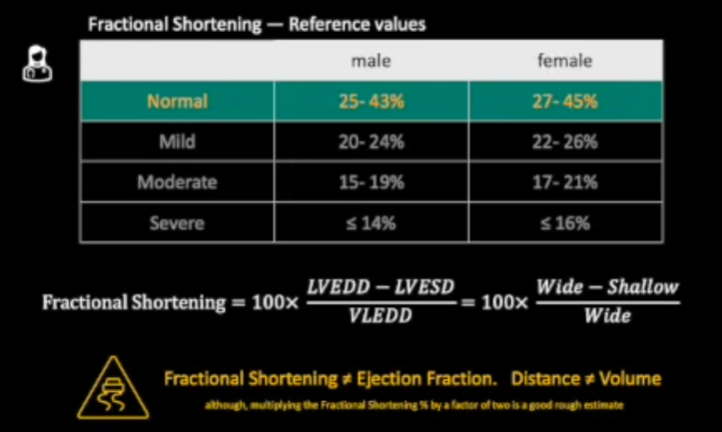
\includegraphics[keepaspectratio]{images/efbyfs.png}}
\pandocbounded{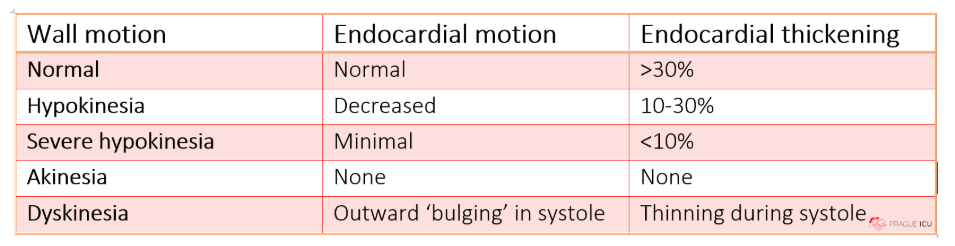
\includegraphics[keepaspectratio]{images/efbythickening.png}}

\subsubsection{Esimerkkejä}\label{Esimerkkeja}

\subsection{EPSS}\label{epss}

\subsection{MAPSE}\label{mapse}

\section{Yleisiä sudenkuoppia}\label{Sudenkuoppia}

Kuten kaikessa ultraäänitutkimukseen liittyvässä, vasemman kammion ulottuvuuksien mittaamisessa ja ejektiofraktion arvioimisessa on monia ongelmakohtia, jotka voivat johtaa tutkijaa harhaan. Yllä ollaan jo puhuttu paljon forshorteningista ja sen vaikutuksista sekä annettu myös muutamia vinkkejä endokardiumin rajojen tunnistamiseen apikaalisissa projektioissa. Käydään läpi vielä muutamia yleisesti tavattavia ongelmia.

\subsection{Paikkalliset liikehäiriöt}\label{Paikalliset-liikehairiot}

\subsection{Dyssynkronia}\label{dyssynkronia}

\subsection{Kammioväliseinämän paksuus - False tendon / Moderator band / Sigmoidi septum}\label{Kammiovaliseinaman-paksuus}

IVS:n mittaamisessa on muutamia ongelmakohtia, joista yleisimpiä ovat septumin läheiset rakenteet, kuten \textbf{false tendonit ja moderator bandit.} Samoin septumin \textbf{sigmoidaalinen tyven paksuuntuminen} on yleinen häiriötekijä.

\subsubsection{False tendon}\label{false-tendon}

False tendon eli valejänne (left ventricular false tendon, LVFT) on pääsääntöisesti vaaraton ja yleinen (esiintyvyys vaihtelee 18\%-83\%) sydämen anatominen variantti, joka sijaitsee vasemmassa kammiossa. Se on fibromuskulaarinen säie, joka kulkee kammion seinämästä toiseen vaikuttamatta sydämen toimintaan. Ne voivat joskus aiheuttaa varsinkin lapsilla harmittomia systolisia sivuääniä säikeiden värinästä johtuen ja todella harvoin ne voivat myös olla rytmihäiriöille altistavia (sisältävät sähköisiä signaaleja välittäviä purkinjen säikeitä). Pääsääntöisesti kuitenkin niiden ainoa kliininen merkitys on niistä aiheutuvat kuvantamishaasteet.

Koska suurin osa false tendoneista kiinnittyy septumiin ja vielä septumin tyveen, niin ne luonnollisesti tulevat PLAX:ssa usein mittauslinjalle. Tällöin se \textbf{pitää osata tunnistaa ja ymmärtää jättää mittaamatta IVS:n paksuutta arvioidessa.} False tendonin huomaa yleensä helposti siitä, että sen ja oikean kammioväliseinän välissä näkyy anekooista verta; kuitenkin joskus säie voi nuolla seinämää hyvinkin läheltä, jolloin tämän tunnistaminen on vaikeaa.

\pandocbounded{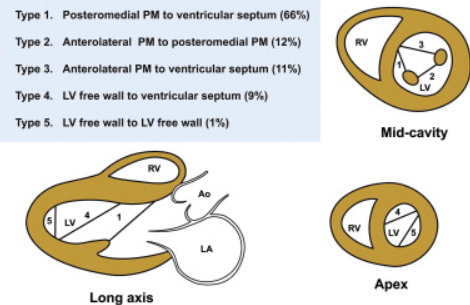
\includegraphics[keepaspectratio]{images/lvfttypes.png}}
\pandocbounded{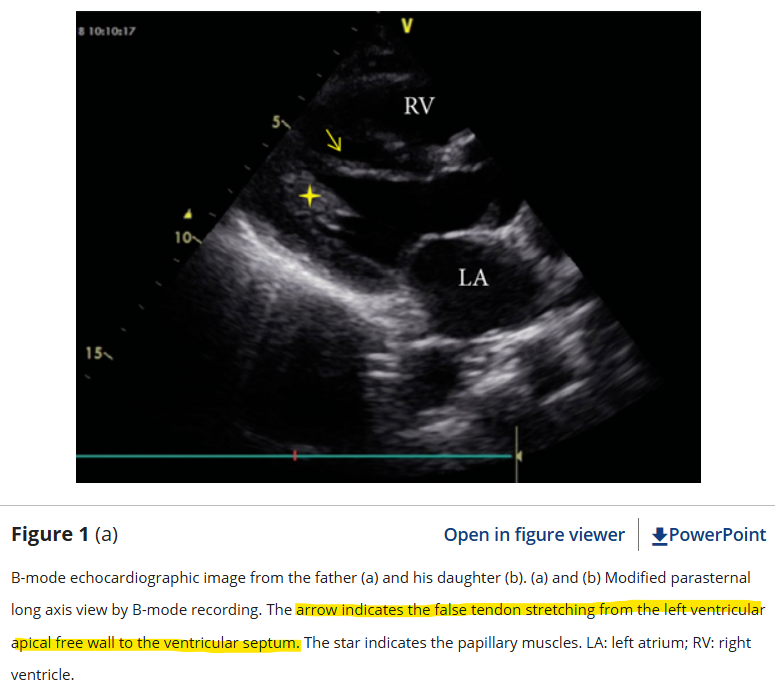
\includegraphics[keepaspectratio]{images/lvftplax.png}}

\subsubsection{Moderator band}\label{moderator-band}

Myös oikealla kammiolla on oma yleinen mittauksia häiritsevä anatominen piirre - moderator band. Se on sydämen oikeassa kammiossa sijaitseva lihasjuoste, jota kutsutaan myös nimellä septomarginaalinen trabekkeli (lat. trabecula septomarginalis). Se on normaalistikin esiintyvä sydänrakenne eikä niinkään anatominen variantti (enemmänkin harvinaista, jos ei ole todettavissa - puuttuu vain n.~10\%:lla). Se kuitenkin ilmenee eri tavalla ei ihmisillä ja joillain se on prominentimpi kun taas joillain vaikeammin havaittavissa.

Moderator bandin pääasiallinen tehtävä on toimia sähköisiä signaaleja kuljettavana linjana. Se vie osan oikean haaran (right bundle branch) signaaleista oikean kammion anterioriseen papillaarilihakseen. Tämä oikoreitti on merkityksellinen, koska se auttaa varmistamaan, että nystylihas supistuu samanaikaisesti muun kammion kanssa, mikä estää kolmiliuskaläppää (trikuspidaaliläppää) vuotamasta systolen aikana. Se myös tukee kammion seinämää ja estää kammiota venymästä liikaa.

Useimmiten moderator band ei kiinnity niin korkealle kammioväliseinämän tyveen, että se häiritsisi IVS:n mittaamista. Kuitenkin joskus näin käy ja moderator band on hyvä osata tunnistaa niin PLAX:sta kuin muistakin näkymistä.

\pandocbounded{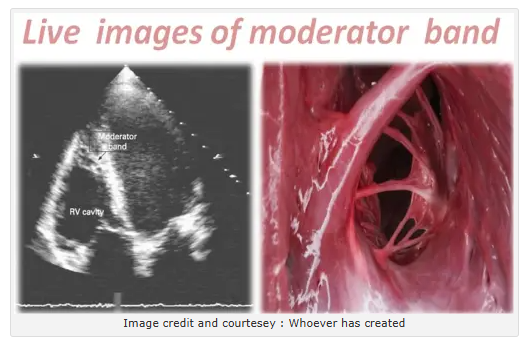
\includegraphics[keepaspectratio]{images/moderatorband1.png}}
\pandocbounded{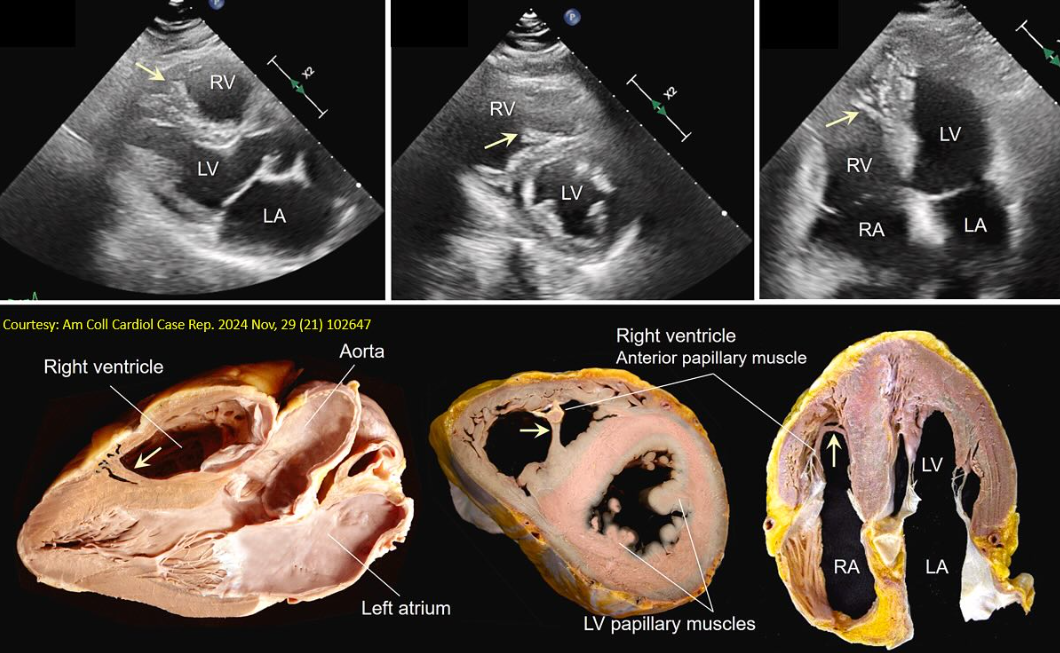
\includegraphics[keepaspectratio]{images/moderatorband2.png}}
\pandocbounded{\includegraphics[keepaspectratio]{images/moderatorbanda4c.gif}}
\pandocbounded{\includegraphics[keepaspectratio]{images/moderatorbandpsax.gif}}

\subsubsection{Sigmoidi septum}\label{sigmoidi-septum}

Sigmoid septum (interventricular septal bulge, discrete upper septal thickening, asymmetric septal hypertrophy) on \textbf{yleinen löydös varsinkin vanhuspopulaatiossa} ja viittaa isoloituun septumin tyven paksuuntumaan, joka ilmenee sigmoidaalisena (S-kirjaimen) muotona. Sigmoidi septum on siis hypertrofisen kardiomyopatian tietty alatyyppi, joka liittyy läheisesti ikääntymiseen ja myös systoliseen verenpaineeseen sekä aorttastenoosiin. Ajatellaan, että korkea verenpaine tai aorttastenoosin tuoma resistenssi kuormittaa erityisesti ulosvirtauskanavan läheistä aluetta ja tämä johtaisi septumin tyviosan paksunemiseen herkästi. Ikääntyminen myös itsessään voi aiheuttaa löydöksen, koska ikääntymiseen liittyvä aortan dilataatio ja pidentyminen johtaa sen siirtymiseen oikealle ja tämä taas aiheuttaa LV:n tyven työntymistä vasemmalle ja LVOT:iin.

Hypertrofinen kardiomyopatia on yleisesti ottaen geneettinen ongelma ja jopa n.~puolella potilaista voidaan todeta kaupallisissa testeissä etsittyjä altistavia mutaatioita (useimmiten sarkomeerigeeneistä). Sigmoidissa septumissa löydetään selittäviä geneettisiä mutaatioita merkittävästi muita morfologisia variantteja harvemmin. Tämän takia sitä ei aina ajatella edes hypertrofiseksi kardiomyopatiaksi, vaan omaksi löydöksekseen, joka liittyy vahvasti ikääntymiseen ja vasemman kammion rasitukseen.

``Oikean'' hypertrofisen kardiomyopatian tunnistaa echossa siitä, että paksuuntuminen on laajempaa ja affisioi myös muita osia kuin septumin tyveä paikallisesti (pääasiassa septumia ja loppuosaa vasemmasta kammiosta)

\pandocbounded{\includegraphics[keepaspectratio]{images/sigmoid.gif}}

\paragraph{Sigmoidin kasvun huomioiminen mittauksissa}\label{sigmoidin-kasvun-huomioiminen-mittauksissa}

Sigmoidi tyven kasvu häiritsee kammioväliseinämän paksuuden ja ejektiofraktion mittaamista merkittävästi. Yleensä sigmoidin septumin kanssa kannattaakin siirtää mittauslinjaa hieman apeksia kohti fokaalisesta paksuuntumisesta poispäin (niin diastolessa kuin systolessa). Fokaalisen paksuuntumisen mittaaminen omana arvonaan on kannattavaa, jotta lausunnosta voi saada paremman käsityksen tilanteesta. Alla esimerkkikuva mittauksista.

\pandocbounded{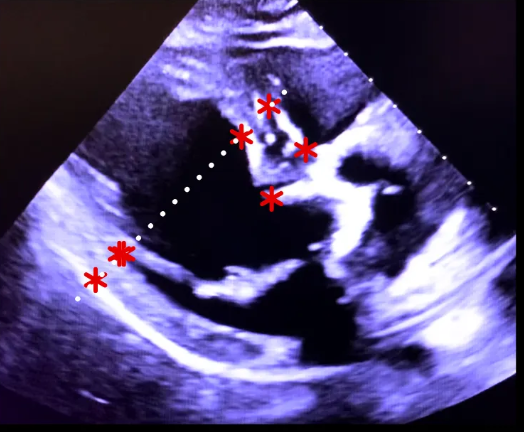
\includegraphics[keepaspectratio]{images/sigmoidseptumhowtomeasure.png}}

\paragraph{Sigmoidin kasvun merkitys}\label{sigmoidin-kasvun-merkitys}

\textbf{Suurimmalle osalle ihmisistä sigmoidi septum on oireeton hyvänlaatuinen anatominen variantti ja vain sivulöydös UKG:ssa.} Sillä voi kuitenkin tietyissä tilanteissa olla kliinistä merkitystä. Kasvu voi aiheuttaa dynaamista \emph{vasemman kammion ulosvirtauskanavan obstruktiota (LVOTO)} varsinkin hyperkontraktiileissa tiloissa tai preloadin ollessa madaltunut (esim. hypovolemia, vasodilataatio, takykardia). Obstruktioon osallistuu vahvasti obstruktiiviseen hypertrofiseen kardiomyopatiaan usein liittyvä mitraaliläpän liike septumiin päin systolessa (SAM-liike; systolic anterior motion).

Virtaukset ulosvirtauskanavassa nopeutuvat, koska kammioväliseinämän tyvi kaventaa ulosvirtauskanavaa (kun neste pakotetaan kapeamman kohdan läpi, sen pitää nopeutua ylläpitääkseen jatkuvaa virtausta). Bernoullin lain mukaan virtauksessa nopeuden kasvaessa paine alenee. Tämä matalapaine aiheuttaa imua (Venturi-ilmiö), joka vetää mitraaliläpän anteriorista purjetta anteriorisesti ulosvirtauskanavaan pahentaen obstruktiota systolessa -\textgreater{} dynaaminen obstruktio.

Tästä tulee venturi-maskien (käytetään lisähapen annostelumekanismina esim. jos happpiviikset eivät riitä) nimikin. Maskiin pumpataan kapean liittimen kautta 100\% happea. Tämä kapean kohdan läpi virtaava happi aiheuttaa venturi-ilmiön kautta imuefektin ja liittimen rei'istä pääsee huoneenilmaa sekoittumaan happivirtaan. Liittimiä ja happivirtauksen nopeutta säätelemällä voidaan muokata lopulta hengitetyn kaasun happipitoisuus sopivaksi potilaalle (yleensä virtaukset välillä 2-15 l/min ja happipitoisuus 28--40 \%).

uudemmissa tutkimuksissa on havaittu, että Venturi-ilmiö ei todennäköisesti riitä yksin selittämään SAM:ia, varsinkaan ei-pelkästään sigmoidaalisissa hypertrofisissa kardiomyopatioissa.

Usein SAM-potilailla on papillaarilihasten anteriorista siirtymistä ja/tai mitraaliläpän purjeiden ekstensoitumista kammioon. Mitraaliläpän purjeiden koaptaatio tapahtuu siis mitraaliannuluksen distaalipuolella ja usein nämä ekstrapitkät purjeet eivät sulkeudu nätisti, vaan niiden sulkeutumispisteen distaalipuolelle jää ylimääräistä löysää kudosta (``residual leaflet'').

Ajatellaan, että epänormaali mitraaliläpän ja papillaarilihasten morfologia altistaa systolessa virtaukselle, joka mekaanisesti työntää mitraaliläppää kohti LVOT:ia.

SAM on siis todennäköisesti yleensä yhdistelmä mekaanista työntöä ja Venturin-ilmiön kautta syntyvää imua

LVOTO pahenee hyperkontraktiileissa tiloissa (esim. rasitus, stressi, lääkkeet yms sympaattista aktivaatiota nostavat tekijät), koska se lisää virtausnopeuksia LVOT:ssa (pahentaa Venturi-ilmiötä) ja myös pahentaa työntöefektiä. Preloadin väheneminen (esim. hypovolemia tai nitraattien aiheuttama vasodilataatio) pahentaa geometrisesti obstruktiota, kun kammion täyttötilavuus pienenee (kammion ontelo jää pieneksi ja supistuksen alkaessa sen seinämät / sigmoidi paksuuntuminen ja mitraaliläpän purjeet ovat anatomisesti lähempänä toisiaan).

Dynaaminen LVOTO voi siis usein tulla esiin vain tällaisissa stressitilanteissa ja olla muuten täysin ongelmaton.

\pandocbounded{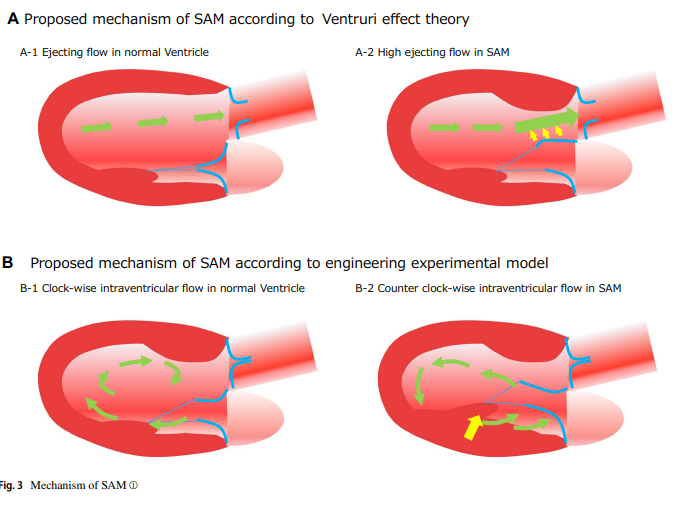
\includegraphics[keepaspectratio]{images/samengineering.png}}
\pandocbounded{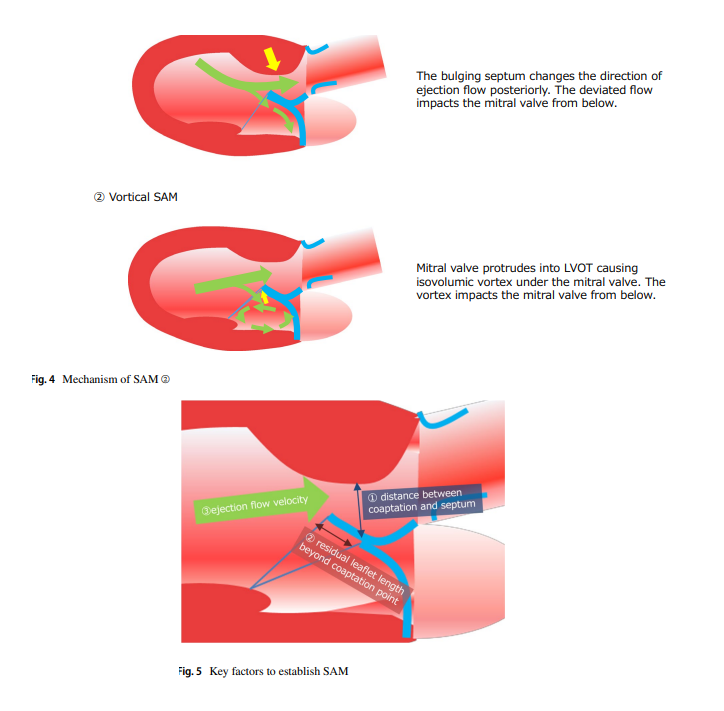
\includegraphics[keepaspectratio]{images/sammechanism.png}}
\pandocbounded{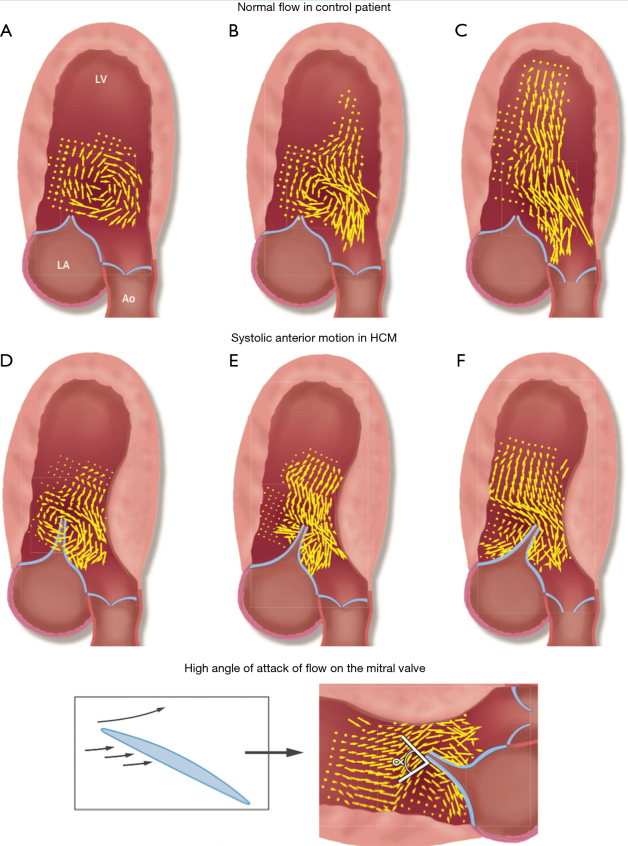
\includegraphics[keepaspectratio]{images/samhcm.png}}
\pandocbounded{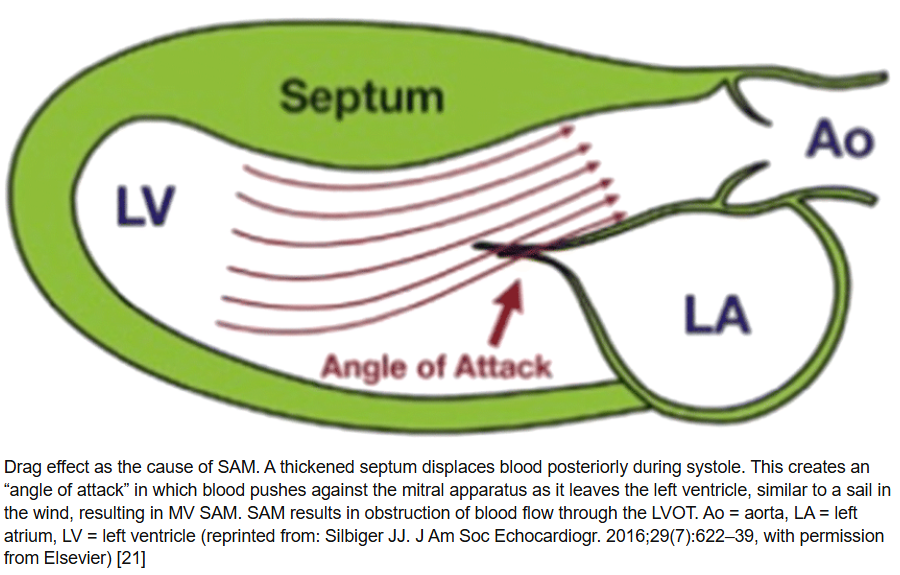
\includegraphics[keepaspectratio]{images/samfrag.png}}
\pandocbounded{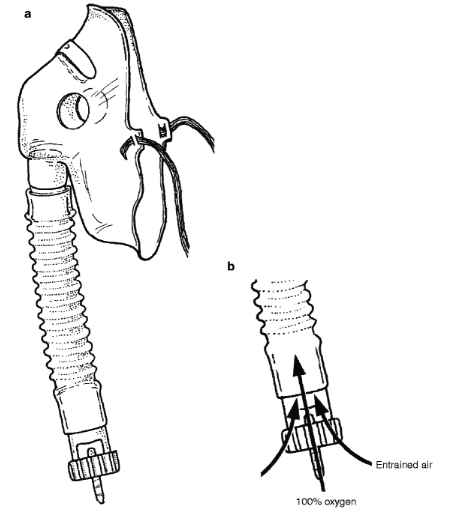
\includegraphics[keepaspectratio]{images/venturimask.png}}

\paragraph{SAM:n tunnistaminen}\label{samn-tunnistaminen}

SAM:n tunnistaminen alkaa sen riskitekijöiden tunnistamisesta. Jos näkee mm. pienen LV:n, merkittävän paksut seinämät, sigmoidin septumin, papillaarilihasten anteriorista siirtymistä, kapean LVOT:n, nopeat LVOT-virtaukset yms., niin kannattaa myös pitää mielessä SAM:n mahdollisuus ja siirtää silmät myös mitraaliläpän alueelle. Samoin kannattaa erityisesti epäillä SAM:n kehittymistä mitraaliläpän korjausleikkausten jälkeen.

\pandocbounded{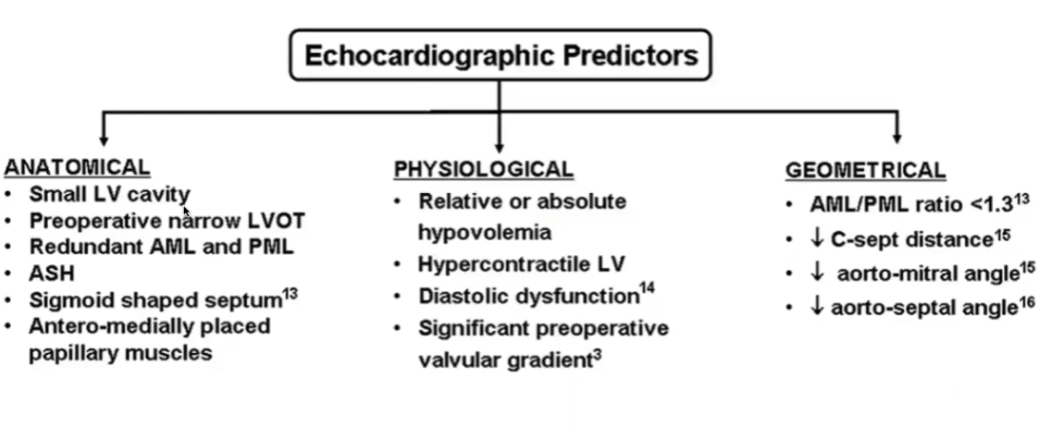
\includegraphics[keepaspectratio]{images/sampredictors.png}}
\pandocbounded{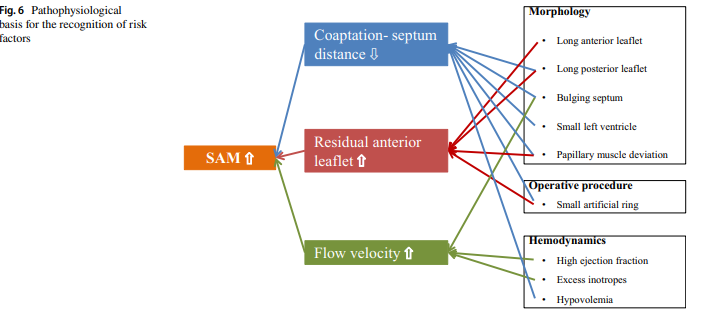
\includegraphics[keepaspectratio]{images/samrisk.png}}

Visuaalisesti SAM:n voi tunnistaa usein pelkällä TTE:llä mm. PLAX- tai A5C (tai A3C)-projektioista.

\pandocbounded{
\includegraphics[keepaspectratio]{images/sama3c.gif}}
\pandocbounded{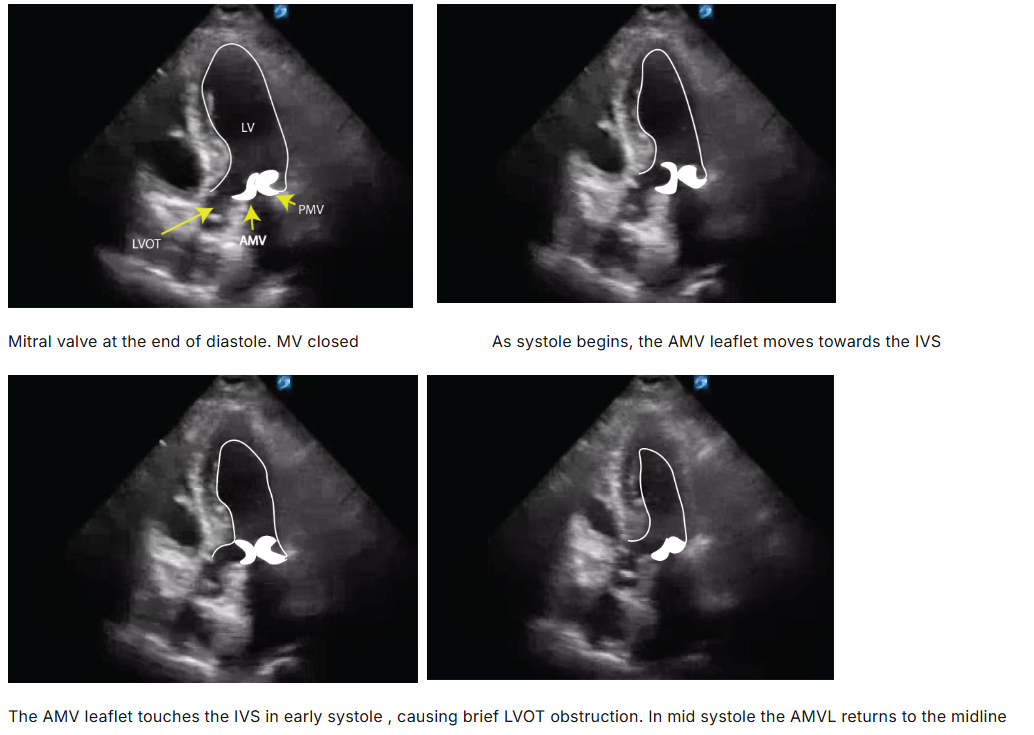
\includegraphics[keepaspectratio]{images/sama3c.png}}
\pandocbounded{\includegraphics[keepaspectratio]{images/samplax.gif}}

Kuten tästä alimmasta gifistä näkee, niin SAM:n tunnistamista (ja graaderausta) voi helpottaa M-moodi mitraaliläpän kärkien läpi PLAX-projektiossa; samalla tavalla kuin EPSS:n voi ottaa ejektiofraktiota arvioidessaan.

\pandocbounded{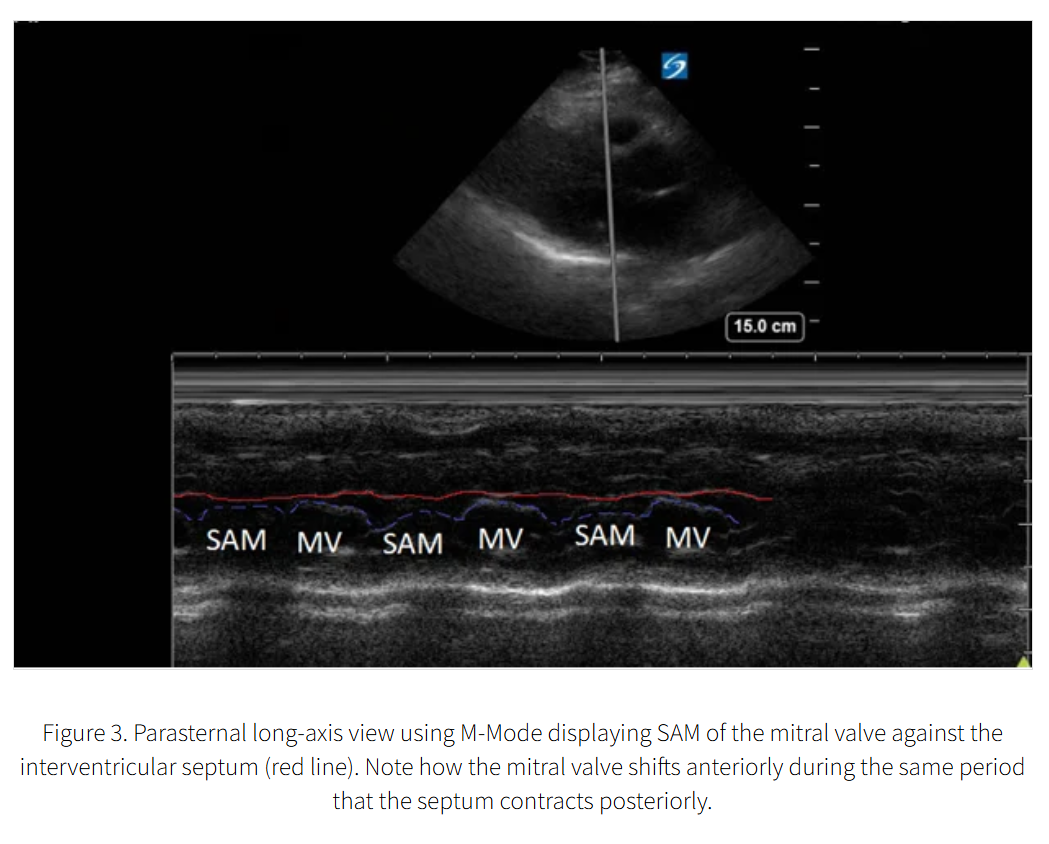
\includegraphics[keepaspectratio]{images/sammode.png}}
\pandocbounded{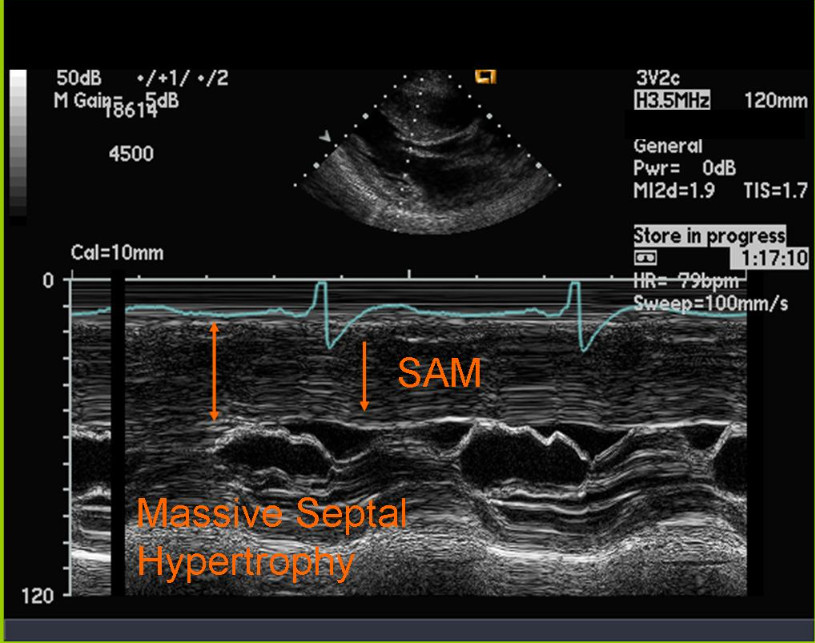
\includegraphics[keepaspectratio]{images/sammode2.png}}
\pandocbounded{\includegraphics[keepaspectratio]{images/g4sam.gif}}
\pandocbounded{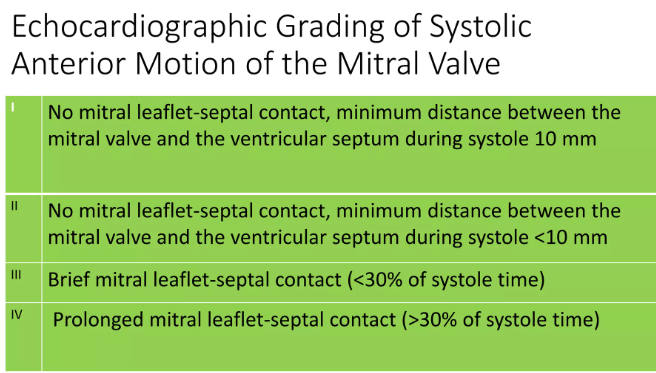
\includegraphics[keepaspectratio]{images/samgrading.png}}

\chapter{Aortta}\label{aortta}

\chapter{Vasen eteinen}\label{vasen-eteinen}

\chapter{Alaonttolaskimo (IVC)}\label{alaonttolaskimo-ivc}

\chapter{Diastoliikka}\label{diastoliikka}

\subsection{Keuhkolaskimovirtaukset}\label{keuhkolaskimovirtaukset-1}

Keuhkolaskimovirtausten arvioimisen yksi indikaatioista on vasemman kammion diastolisen dysfunktion arvioiminen (ei tosin toimi tärkeimpänä tai ensisijaisena mittarina, vaan pikemminkin harvemmin käytettynä tukevana arviona). Toinen yleinen käyttö on esim. mitraalivuodon gradeeraus (siinäkin tukeva parametri). Koska diastoliikka tulee tässä oppaassa mitraalivuotoa ennen, niin käsitellään nyt keuhkolaskimovirtausten mittaaminen ja tulkitseminen. Jo aikaisemmin käytiin läpi keuhkolaskimoiden tunnistaminen ja löytäminen eri projektioista, mutta nyt voidaan tiivistää aihe siihen, että pitää osata löytää apikaalisesta nelilokeroprojektiosta (A4C) oikea ylempi keuhkolaskimo (RUPV; periaatteessa myös oikea alempi laskimokin käy, mutta RUPV on yleensä helpompi löytää). Siitä tyypillisimmin tehdään keuhkolaskimovirtausten mittaukset.

Tässä alla on esimerkki RUPV:n väridopplerista ja mittauspisteestä PW-dopplerin suhteen (oikeanpuoleisin video). Taas kannattaa muistaa, että Nyquistin rajan kannattaa useimmiten olla normaalia hieman matalampi johtuen keuhkolaskimoiden hitaammasta virtauksesta. Yleensä n.~40cm/s tai alle mahdollistaa tarkimman ja parhaimman virtausvisualisaation. Sample gate tulisi siis olla n.~0.5-2cm suonen sisällä eli siis proksimaalisesti sen junktiosta vasemman eteisen kanssa. Yritä suunnata UÄ-aallot mahdollisimman hyvin samansuuntaisiksi virtauksen kanssa.

\pandocbounded{\includegraphics[keepaspectratio]{images/rupvsample.gif}}
\pandocbounded{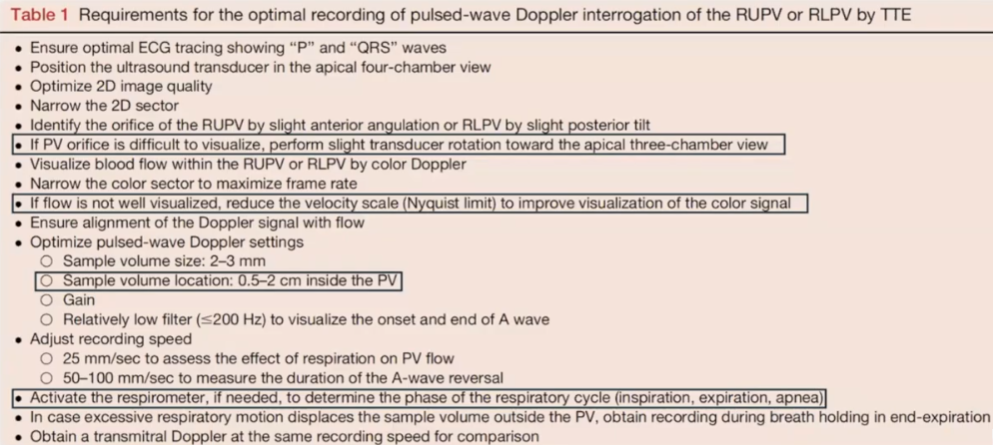
\includegraphics[keepaspectratio]{images/tipspvmeasurement.png}}

Tämä mittaus tuottaa pulssiaaltokäyrän, joka normaalitilanteessa koostuu kolmesta (tai neljästä) pääkomponentista: systoliset deflektiot (S-aalto; usein voi erottaa S1 ja S2) ja diastoliset deflektiot eli D-aalto ja Ar-aalto.

Ensiksi kannattaa tunnistaa Ar-aalto eli atrial reversal

Ar siis ilmenee negatiivisena deflektiona, koska virtaus kulkee keuhkolaskimoon poispäin anturista eikä eteiseen, kuten muut positiiviset deflektiot. Virtauksen kääntyminen vastavirtaan johtuu eteisten kontraktoitumisesta (vastaa täten ajoitukseltaan mitraalivirtauksen A-aaltoa ja EKG:n P-aaltoa). Diastolen lopussa vasen eteinen siis supistuu (eteissystole) työntääkseen viimeisen verimäärän kammioon. Koska keuhkolaskimoiden suilla ei ole mekaanisia läppiä, verta puristuu paineesta johtuen taaksepäin takaisin keuhkolaskimoihin.

Ar-aallosta voi havainnoida sen amplitudin ja keston (Ar duration)

Eteisvärinä on yleinen Ar-aaltoa muokkaava tekijä ja erityisesti se laskee Ar-aallon huippunopeutta, koska eteisvärinässä ei ole synkronoitua eteiskontraktiliteettia. Usein ei ole edes selkeitä Ar-aaltoja eteisvärinässä.

\begin{center}\rule{0.5\linewidth}{0.5pt}\end{center}

Ar-aallon jälkeen seuraava positiivinen deflektio on S-aalto eli systolic wave, joka on usein kaksivaiheinen ja voidaan jakaa osiin S1 ja S2. Useimmiten (n.70\%:lla ihmisistä; varsinkin terveillä nuorilla sekä myös nopeassa sykkeessä) kuitenkin aallot ovat assimiloituneet ja on todettavissa vain yksi S-aalto.

S1 eli alkusystolinen aalto syntyy kammiosystolen alussa eli eteissystolen päätyttyä, kun vasen eteinen alkaa rentoutua (eteisdiastole). Tämä luo eteiseen imuefektin ja paine laskee, jolloin veri syöksyy laskimoista eteiseen.

Varsinkaan eteisvärinässä S1 ei ole havaittavissa epäkoordinoidun eteistoiminnan takia. S1-aaltoon vaikuttaa myös LA:n relaksaatiokyky (heikko relaksaatiokyky laskee S1-aaltoa) ja eteisen kontraktiliteetti (isompi kontraktiliteetti -\textgreater{} parempi täyttyminen supistumisen jälkeen (Frank-Starlingin laki).

S2 eli loppusystolinen aalto syntyy kammiosystolessa mitraaliannuluksen siirtyessä apikaalisesti, mikä taas laskee vasemman eteisen painetta entisestään ja luo gradienttia virtaukselle eteiseen. Samalla oikean kammion luoma perfuusio keuhkoihin päin voi työntää taas lisääntyneen keuhkovaltimopaineen seurauksena laskimoverta eteenpäin (pushing effect).

Oikean kammion toiminta täten voi vaikuttaa S2-aaltoon (RV stroke volumen laskiessa S2 laskee). Samoin LV:n pitkittäissupistuvuus vaikuttaa (vaikuttaa mitraaliannuluksen siirtymiseen) ja tietysti myös LA:n komplianssi vaikuttaa S2-aaltoon.

\begin{center}\rule{0.5\linewidth}{0.5pt}\end{center}

Systolisten aaltojen jälkeen seuraava käyrän huippu kuvastaa D-aaltoa eli diastolista aaltoa.

D-aalto kuvastaa eteisten tyhjenemistä eli se syntyy, kun mitraaliläppä avautuu. Tällöin veri virtaa nopeasti vasemmasta eteisestä suoraan vasempaan kammioon. Tämä tyhjentää eteisestä painetta, jolloin keuhkolaskimoista pääsee virtaamaan uutta verta vapaasti suoraan eteisen läpi kammioon. D-aalto vastaa ajoitukseltaan ja logiikaltaan suoraan mitraalivirtauksen E-aaltoa (kammion varhaisdiastolinen täyttyminen).

Tietysti siihen taas vaikuttaa LV:n relaksaatiokyky ja LV:n komplianssi

\begin{center}\rule{0.5\linewidth}{0.5pt}\end{center}

On siis hyvä tiedostaa, että pulmonaalilaskimoiden virtauksiin vaikuttavat monet hemodynaamiset ja sydämen rakenteelliset tekijät.

\pandocbounded{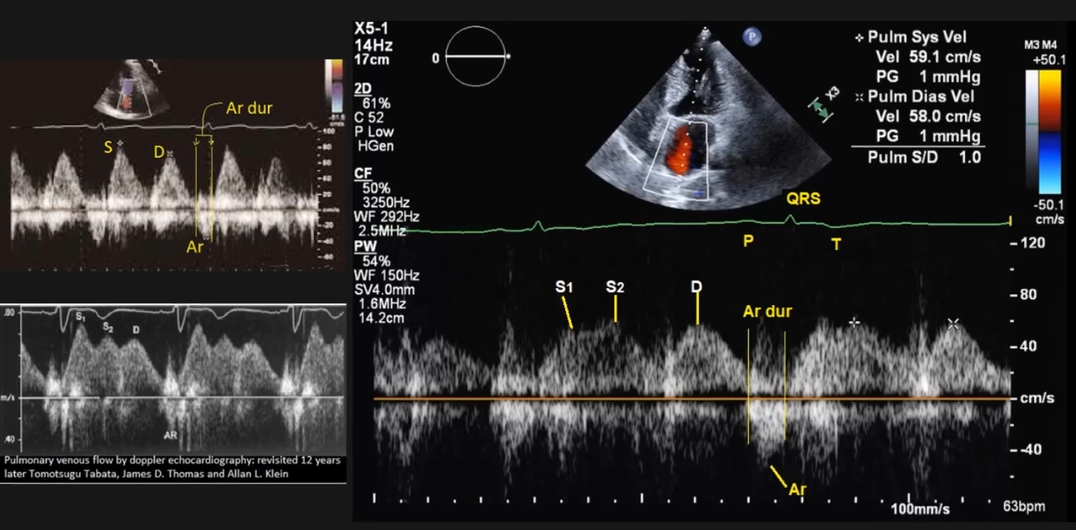
\includegraphics[keepaspectratio]{images/pvdopplerpattern.png}}
\pandocbounded{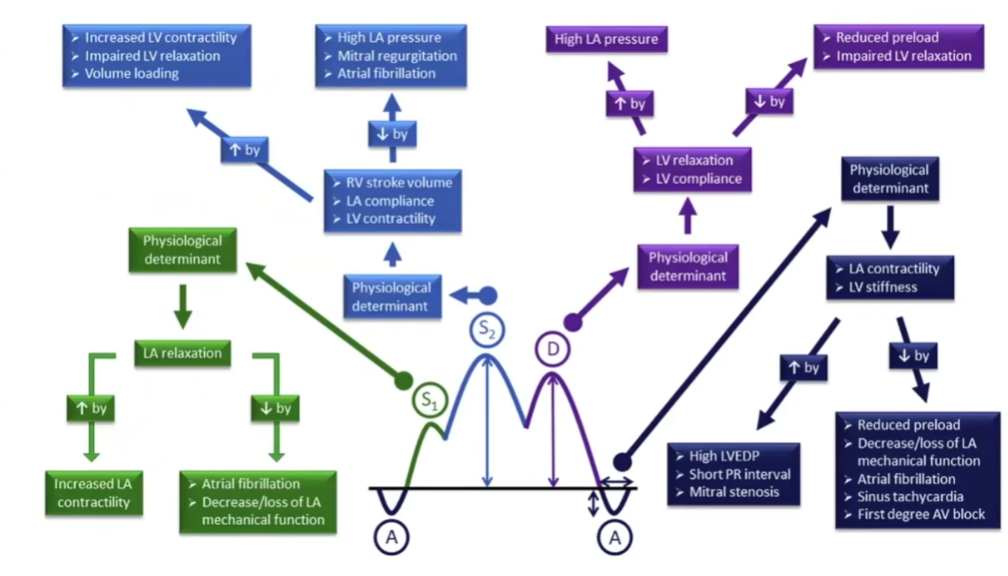
\includegraphics[keepaspectratio]{images/pulmonaryveindeterminants.png}}

\subsubsection{Keuhkolaskimovirtaukset diastoliikassa}\label{keuhkolaskimovirtaukset-diastoliikassa}

Diastoliikassa keuhkolaskimovirtauksista useimmiten arvioidaan pääasiassa S/D-suhdetta. Yleensä normaaliksi suhteeksi ilmoitetaan, että S-aalto on suurempi (jos sekä S1 että S2 ovat nähtävissä, niin mitataan S2) tai yhtä suuri kuin D-aalto amplitudiltaan (S/D ≥ 1) eli normaalit täyttökuviot (filling patterns) ovat vahvemmin systolisia ja patologiset löydökset diastolisen vajaatoiminnan suhteen olisivat S/D \textless{} 1. Suhteen tulkitsemiseen kuitenkin vaikuttaa merkittävästi potilaan ikä, joten yksittäistä ``normaalia'' arvoa ei voi suoraan antaa.

Nuorilla (n.~\textless{} 40v) ja terveillä potilailla voi S/D-suhde olla hyvinkin alle 1 ilman mitään ongelmaa sydämessä. Todella hyvä elastinen rekoili ja nopea vasemman kammion relaksaatio mahdollistaa sen, että aikaisin diastolessa tapahtuva vasemman kammion täyttyminen on hyvin tehokasta ja sydämen ei tarvitse turvautua eteissystoleen (mitraalivirtauksen A-aalto ja keuhkolaskimovirtausten Ar-aalto) kovinkaan paljoa. Tämä näkyy siis myös mitraalivirtausten E- ja A-aalloissa; A-aalto voi olla aika pieni ja E-aalto on suuri siihen verrattuna -\textgreater{} nuorilla ja urheilullisilla ihmisillä voi E/A-suhde olla hyvinkin yli 2, vaikka se on tyypillisen ``normaalin'' yläraja.

D-aalto voi siis olla systolista virtausta prominentimpi tehokkaan diastolisen täyttymisen takia ja eteissystolea ei tarvita merkittävissä määrin (ja täten eteisten täyttyminen supistumisen jälkeen vähenee (Frank-Starlingin lain mukaan vähäisempi supistus johtaa vähäisempään relaksaatioon ja siten vähäisempään imutoimintaan) -\textgreater{} S/D \textless{} 1 ja pieni Ar-amplitudi

Henkilön ikääntyessä (n.~ikävuodet 30-40+) tapahtuu normaalia vasemman kammion relaksaatiokyvyn laskua. Tämä johtaa progressiiviseen LV:n aikaisdiastolisen täyttymisen vähenemiseen ja myös siten eteissystolessa siirrettävän veren määrän nousuun -\textgreater{} S- ja D-aaltojen amplitudit tasoittuvat. Vielä ikääntymisen edetessä lopulta S-aallosta tulee suurempi kuin D-aallosta -\textgreater{} S/D-suhde \textgreater{} 1 (ja Ar-aalto on prominentti).

Tämä ei ole diastolista vajaatoimintaa, vaan normaalia ikääntymistä. Periaatteessa tämä peilautuu gr 1 diastoliseksi dysfunktioksi - samoin kuten E/A-suhde alle 0.8 ikääntyessä

\begin{center}\rule{0.5\linewidth}{0.5pt}\end{center}

Jos ultraa \textgreater40-vuotiasta, niin voi yleensä ajatella normaalin S/D-suhteen olevan \textgreater{} 1. Tässä potilaskunnassa S/D \textless{} 1 on yleensä patologista (vaikka onkin samalla tasolla kuin terveillä nuorilla; tämä taas peilautuu gr 2-3 diastoliseen dysfunktioon ja E/A suhteen pseudonormalisaatioon) ja kuvastaa vasemman eteisen paineiden nousua. LA:n paineiden noustessa esim. juuri diastolisesta vajaatoiminnasta johtuen vähenee S-aallon nopeudet, koska kohonneet paineet eteisessä aiheuttavat resistenssin tulevaa keuhkolaskimovirtausta vastaan. Mitraaliläpän avautuessa diastolessa tämä korkea paine aiheuttaa nopean virtauksen ventrikkeliin (samalla periaatteella E-aalto nousee mitraalivirtauksia tutkiessa) ja siten myös tehokkaan samanaikaisen eteisen täyttymisen ja korkean D-aallon.

\begin{center}\rule{0.5\linewidth}{0.5pt}\end{center}

Pähkinänkuoressa voi siis ajatella keuhkolaskimovirtauksista näin: D-aalto käyttäytyy samalla tavalla kuin mitraalivirtauksen E-aalto eli se kasvaa ja terävöityy diastolisen vajaatoiminnan edetessä -\textgreater{} E/A-suhde nousee ja S/D-suhde laskee.

\pandocbounded{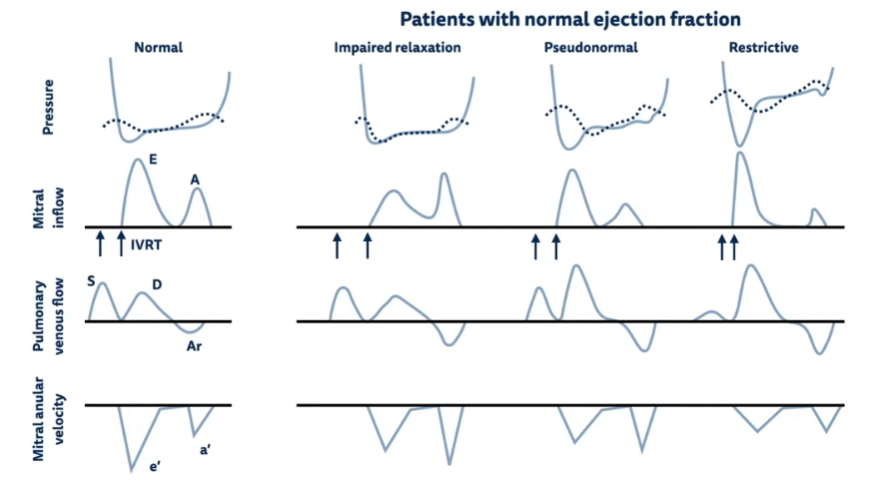
\includegraphics[keepaspectratio]{images/eapv.png}}

\pandocbounded{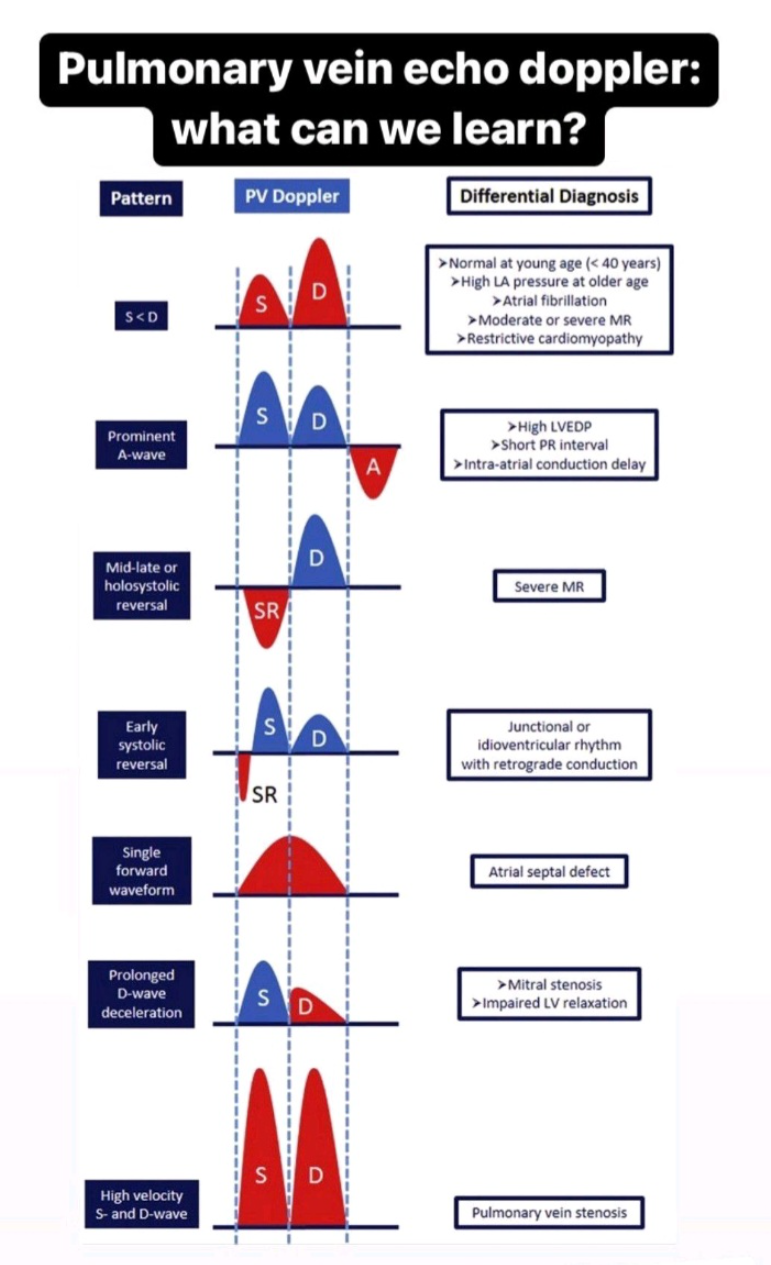
\includegraphics[keepaspectratio]{images/whatcanwelearn.png}}

\chapter{Aorttastenoosi}\label{aorttastenoosi}

\chapter{Sydämen oikea puoli}\label{syduxe4men-oikea-puoli}

\chapter{Mitraalivuoto}\label{mitraalivuoto-1}

Hiippaläppävuoto on länsimaisessa väestössä yleisin läppävika ja toiseksi yleisin läppäkirurgian aihe aorttastenoosin jälkeen. Yli 75-vuotiaasta väestöstä jopa vajaalla 10 \%:lla on keskivaikea tai vaikea hiippaläppävuoto, ja onkin ilmeistä, että se on alihoidettu sairaus.

\section{Läppävuodon anatomia}\label{Lappavuodon-anatomia}

Läppävuodoilla (ei siis pelkästään mitraalivuodolla) on tyypillinen rakenne, joka on hyvä tunnistaa, koska sen osien mittaamiseen perustuu monet vaikeusasteen määrittämisessä käytettävät arvot.

\textbf{Vuodot koostuvat siis kolmesta osasta: virtauksen kiihtyvyysalue (konvergenssialue, the flow convergence zone), vuodon kaula (vena contracta, VC) ja vuotosuihkun pinta-ala (jet area).}

\pandocbounded{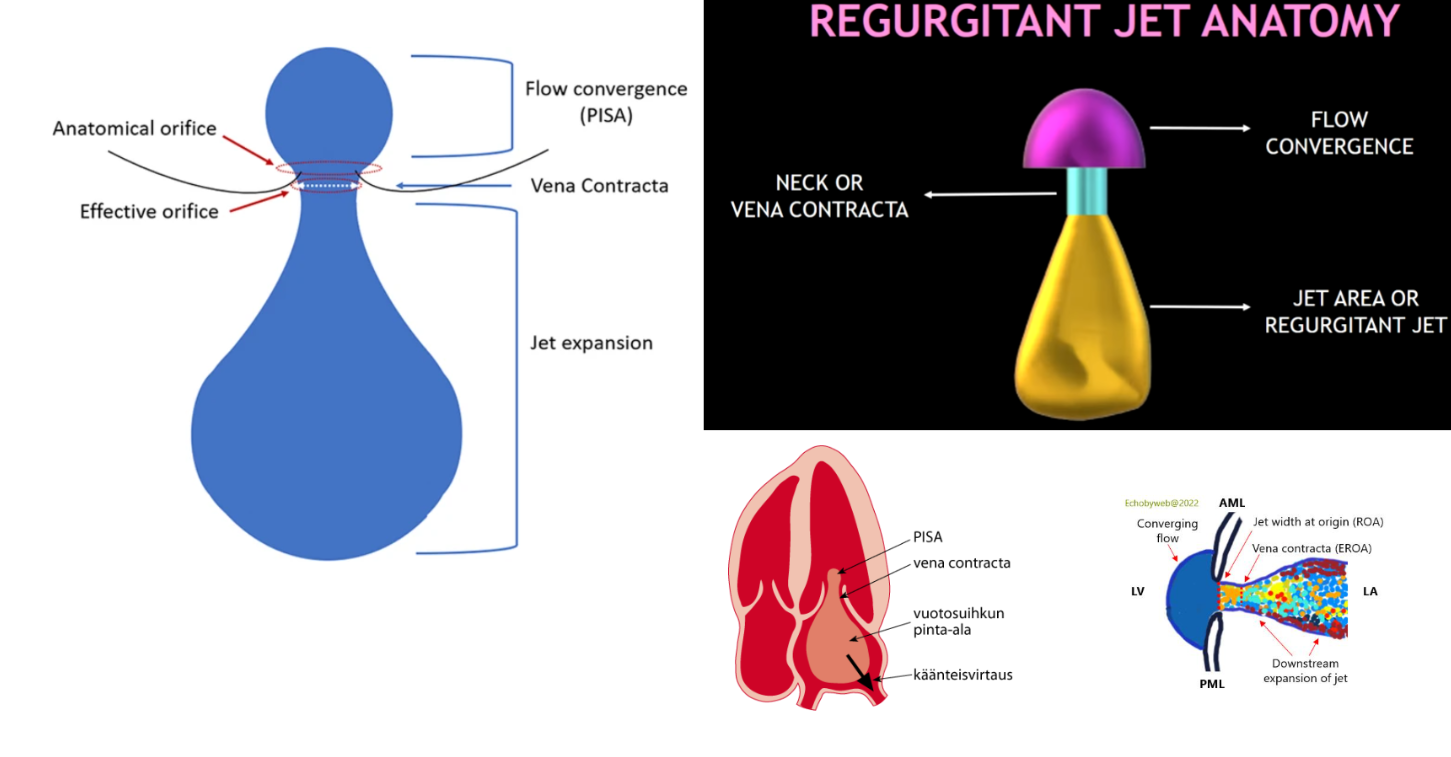
\includegraphics[keepaspectratio]{images/vuotoanatomia.png}}
\pandocbounded{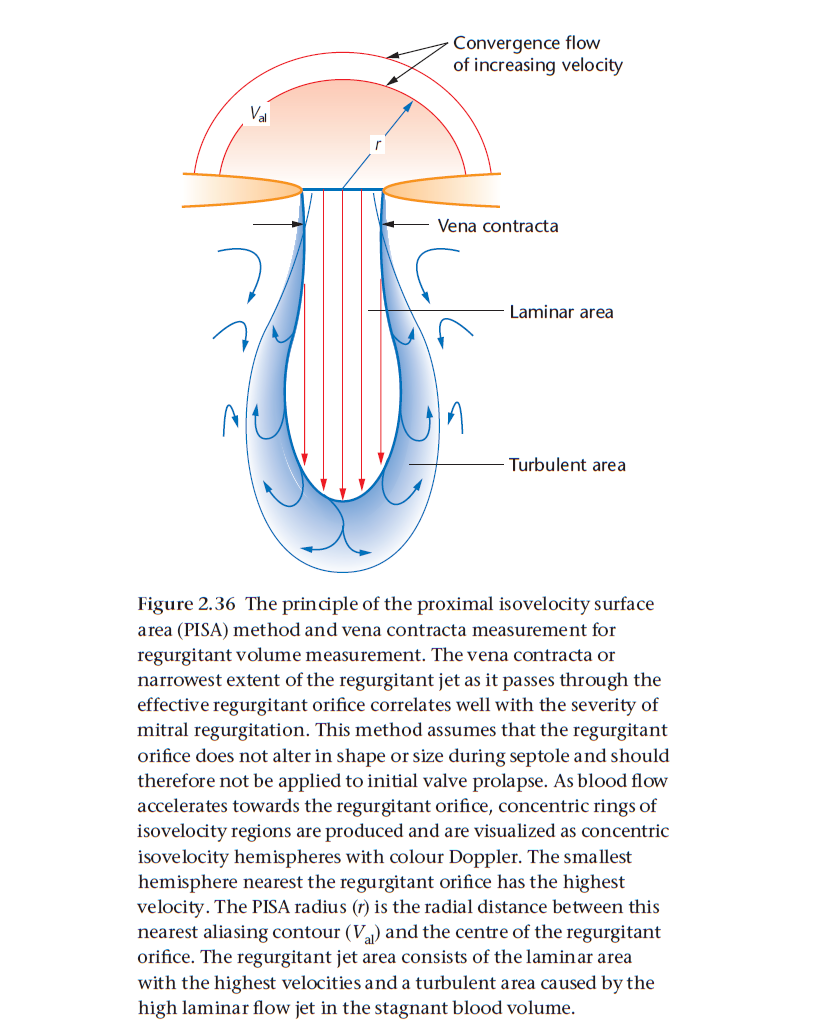
\includegraphics[keepaspectratio]{images/pisa.png}}

\subsection{Virtauksen kiihtyvyysalue (Konvergenssialue), PISA}\label{virtauksen-kiihtyvyysalue-konvergenssialue-pisa}

Vuotovirtauksen konvergenssialue perustuu hemodynaamiseen periaatteeseen, jonka jokainen on varmasti nähnyt toiminnassa jossain muodossa omassa elämässään. Kuvittele tilanne, jossa lavuaari tai kylpy on täynnä vettä ja vedät tulpan pois. Vesi ei liiku vain suoraan alaspäin, vaan suppilomaisesti joka puolelta kohti viemäriaukkoa, ja virtauksen vauhti kiihtyy mitä lähemmäs aukkoa tullaan. Virta siis suuntautuu samaan pisteeseen ja tätä konvergenssi juuri tarkoittaa (konvergenssi = yhteen suuntautuminen, lähentyminen, sulautuminen yms.).

Sydämessä tapahtuu sama asia verelle vuotavien läppien kanssa kuin lavuaarissa vedelle. Kun veri virtaa laajasta sydänlokerosta (esim. vasemmasta kammiosta) kohti kapeaa vuotoaukkoa (esim. vuotavaa hiippaläppää), virtausnopeus kiihtyy asteittain. Tämä kiihtyvyys muodostaa vuotoaukon ympärille samankeskisiä, puolipallon muotoisia vyöhykkeitä, joissa kaikissa on sama virtausnopeus. Näitä kutsutaan isovelositeettipinnoiksi. Tästä tuleekin konvergenssialueen toinen nimi, jota käytetäänkin ensisijaisena nimityksenä kliinisessä työssä: \textbf{PISA eli Proximal Isovelocity Surface Area.}

PISA-periaate sisältää kaksi ajatusta: 1) Virtauksen nopeudet ovat samoja samalla etäisyydellä vuodon aukosta ja 2) Mitä suurempi vuotoaukko on, sitä korkeampia virtaukset ovat tietyllä etäisyydellä aukosta

Vuodon maksiminopeuden määrää pääasiassa paine-ero niiden kahden lokeron välillä, joiden välillä vuoto tapahtuu. Tätä kuvastaa fysiikassa Bernoullin yhtälö: ΔP = 4v\^{}2. Esimerkiksi jos vasemman kammion paine on sydämen supistuessa 120 mmHg ja vasemman eteisen paine on 20 mmHg, lokeroiden välinen paine-ero eli ΔP on 100 mmHg. Tämä 100 mmHg paine-ero pakottaa veren liikkumaan aina noin 5 m/s nopeudella -- oli läpässä oleva reikä sitten nuppineulan pään kokoinen tai peukalon paksuinen (kunhan sydänlihas vain jaksaa ylläpitää tuon paineen).

UÄ-laitteella tosin kylläkin mitataan vuodon nopeus ja siitä kone laskee gradientin -- ei toisinpäin.

Vaikka suuriaukkoisessa vuodossa suihkun maksiminopeus aukon kohdalla pysyy samana, suuri aukko muuttaa tilanteen täysin sen ympärillä eli juuri kiihtyvyysalueella (PISA). Tämä johtuu parista syystä:

Suurempi tilavuus vaatii tilaa: Koska aukko on suuri, sen läpi täytyy mahtua sekunnin murto-osassa suurempi tilavuus verta

Imu ulottuu kauemmas: Jotta tämä suuri määrä verta ehtii suppilomaiseen aukkoon, imuvaikutus ulottuu paljon laajemmalle ja kauemmas sydänlokeroon

\textbf{Iso vuotoaukko ei siis tee itse vuotosuihkun huipusta nopeampaa, vaan se laajentaa kiihtyvyysaluetta. Koska veri alkaa kiihtyä kohti aukkoa paljon kauempana, virtaukset ennen vuotoaukkoa ovat mitattuna nopeampia kuin pienessä vuodossa.} Juuri tämän vuoksi doppleria käyttämällä voi tietää jo jotain vuodon vaikeusasteesta pelkästään kiihtyvyysalueen (PISA) kokoa katsomalla. Tarkempi arvio vuodon vaikeudesta saadaan myös muita vuodon osia tarkastelemalla.

\pandocbounded{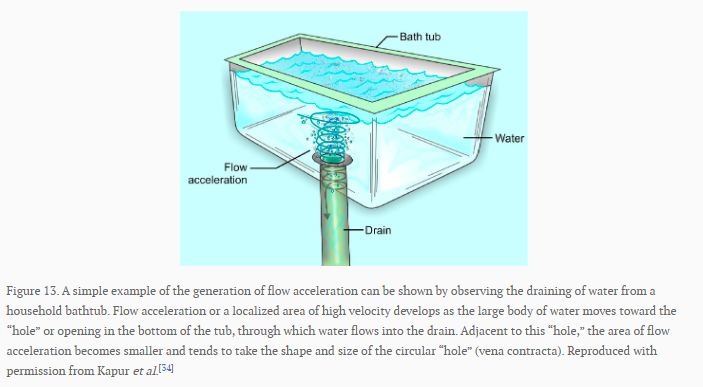
\includegraphics[keepaspectratio]{images/flowconvergencebathtub.png}}
\pandocbounded{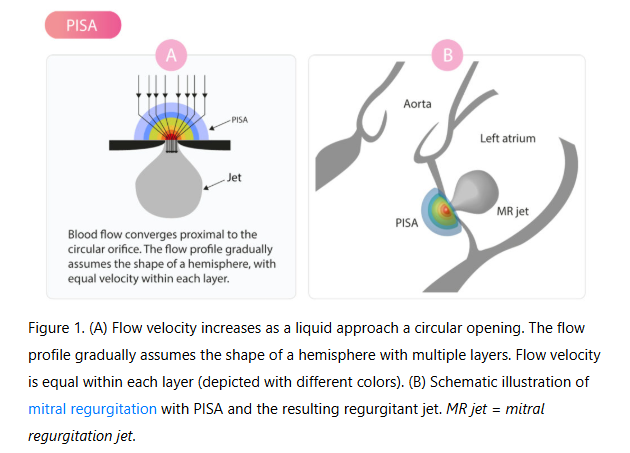
\includegraphics[keepaspectratio]{images/pisarings.png}}

\subsection{Vuodon kaula (vena contracta)}\label{vuodon-kaula-vena-contracta}

Vuodon kaula (vena contracta) on kiihtyvyysalueen (PISA) ja vastaanottavaan sydänlokeroon leviävän varsinaisen vuotosuihkun väliin jäävä vuotosuihkun kapein kohta. Moni pohtii, miksi ei mitata vain itse fyysistä reikää läpän rakenteesta. Se on kuitenkin usein anatomisesti niin epäsäännöllinen, että sitä on äärimmäisen vaikea erottaa luotettavasti perinteisessä ultraäänikuvassa.

Vena contracta kuvaa vuotoaukon jälkeistä nopea- ja laminaarivirtauksista vuodon osaa. Virtaus siis jatkaa lähentymistä vielä pienen hetken senkin jälkeen, kun veri on jo fyysisesti ohittanut mekaanisen läppäaukon, koska virtaavalla verellä on sisäänpäin viettävää liikemäärää eikä sitä pystytä inertian takia heti lopettamaan. Tästä syystä vuotosuihkun kapein kohta muodostuu vasta hitusen aukon jälkeen. Tämä kohta vastaa yleensä lähes täydellisesti läpän tehokasta vuotoaukkoa (EROA, Effective Regurgitant Orifice Area), koska sisäänpäin suuntautuva virtauksen liike aukon jälkeen on todella pientä; vuodon muoto kylläkin vaikuttaa korrelaation vahvuuteen. Ongelmakohtia ovat myös monet vuotosuihkut ja esim. mitraalivuodon tapauksessa non-holosystoliset vuodot.

On siis hyvä tiedostaa, että läppävuoto voi olla mm. pyöreä tai elliptinen

Primaarinen mitraalivuoto on yleensä sirkulaarinen ja tällaisessa tilanteessa vena contracta yleensä kuvastaa vuotoaukon aluetta tarkasti

Primaarinen mitraalivuoto tarkoittaa rakenteellista vuotoa, joka johtuu läppäliuskojen, jännerihmojen tai papillaarilihasten rakenneviasta. Yleisimmät syyt ovat mitraaliläpän prolapsi (kehittyneissä maissa) ja reumaattinen mitraalivuoto (kehitysmaissa). Myös mm. endokardiitti kannattaa pitää mielessä ja etsiä vegetaatioita.

\textbf{Sekundaarinen mitraalivuoto taas on useimmiten elliptinen (slit-shaped) ja tämä johtaa siihen, että vena contracta aliarvioi vuodon vaikeuden.}

Sekundaarinen vuoto tarkoittaa toiminnallista vuotoa ja on seurausta vasemman kammion toimintahäiriöstä tai epänormaalista rakenteesta, joka häiritsee läpän toimintaa; esim. dilatoiva kardiomyopatia tai iskeeminen sydänsairaus (papillaarilihasiskemia)

Vaikka monissa lähteissä sanotaan, että mitraalivuodon VC voitaisiin mitata vain PLAX-ikkunasta, niin vuodon kaula kannattaa kylläkin arvioida myös vähintään A4C-projektiosta, jotta saa paremman arvion siitä, vaihteleeko kaulan leveys kuvausakselin muuttuessa (viittaa siihen, että vuotoaukko ei ole täysin ympyrämäinen). Eri mittaukset voi sitten dokumentoida lausuntoon ja antaa paremman arvion aukon oikeasta koosta.

Vuotoaukon ei-ympyrämäiset muodot häiritsevät myös PISA:a, koska ei-ympyrämäinen aukko johtaa ei-ympyrämäiseen PISA:an.

\pandocbounded{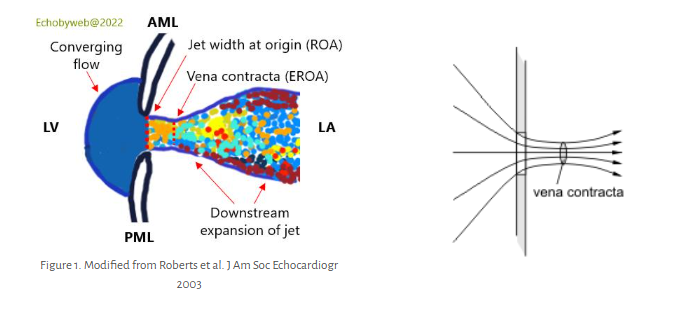
\includegraphics[keepaspectratio]{images/venacontracta.png}}
\pandocbounded{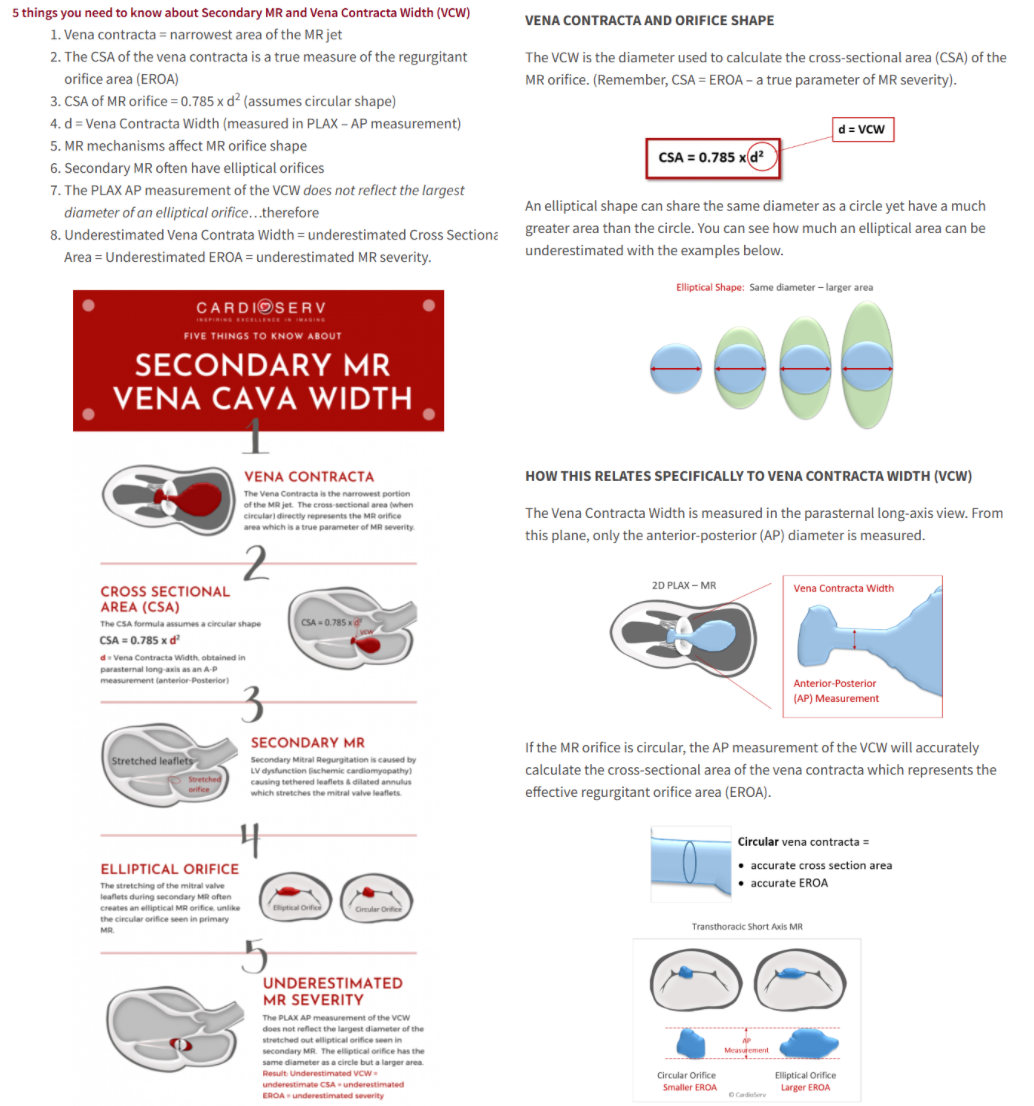
\includegraphics[keepaspectratio]{images/circularvselliptical.png}}

\subsection{Vuotosuihku}\label{vuotosuihku}

Vuotosuihkulla tarkoitetaan itse vuotoaukon jälkeistä turbulenttia virtausta. Tärkein mitta kerätä vuotosuihkusta on vuodon maksimaalinen nopeus (Vmax), sillä sitä tarvitaan EROA:n laskemiseen. Voi myös olla järkevää mitata vuodon VTI (velocity time integral), jonka avulla voidaan laskea vuodon tilavuus. Vuotokäyrän tiheyttä ja muotoa voi myös arvioida.

Vuotoa kannattaa myös arvioida visuaalisesti. Ainakin kannattaa arvioida, onko vuoto sentraalinen (suoraan eteiseen) vai eksentrinen (enemmänkin eteisen seinämiin kohdistuva). Vuodon pinta-alan suhde vasemman eteisen pinta-alaan (visuaalisesti) on monesti käytetty tapa nopeasti arvioida vuodon vaikeutta, mutta se ei ole kovinkaan suositeltu (ainakaan ainoana arviona), koska sen antama arvio riippuu pitkälti koneen asetuksista, vuotomekanismista, hemodynaamisesta tilasta ja vuodon suunnasta.

Eksentrisistä vuodoista on hyvä tiedostaa se, että vuodon läheisyys seinämään voi johtaa Coandăn ilmiöön (virtauksen pyrkimys kääntyä kohti sitä lähellä olevaa pintaa) ja siten vuotosuihku voi näyttää pienemmältä kuin se oikeasti on.

Sentraalisten vuotojen kanssa voi vieläkin joidenkin guidelinejen mukaan periaatteessa hyödyntää vuotosuihkun pinta-alan ja vasemman eteisen välistä suhdetta päättelyn tukena, kun arvioi onko vuoto vaikea-asteinen. Tälle ei kuitenkaan tulisi antaa liikaa painoarvoa.

\pandocbounded{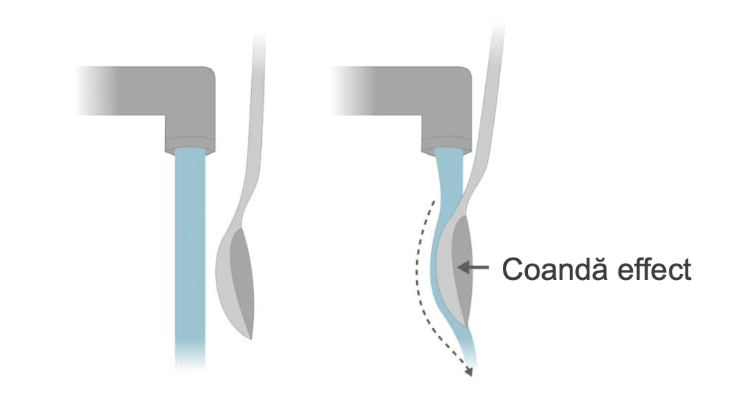
\includegraphics[keepaspectratio]{images/coanda.png}}
\pandocbounded{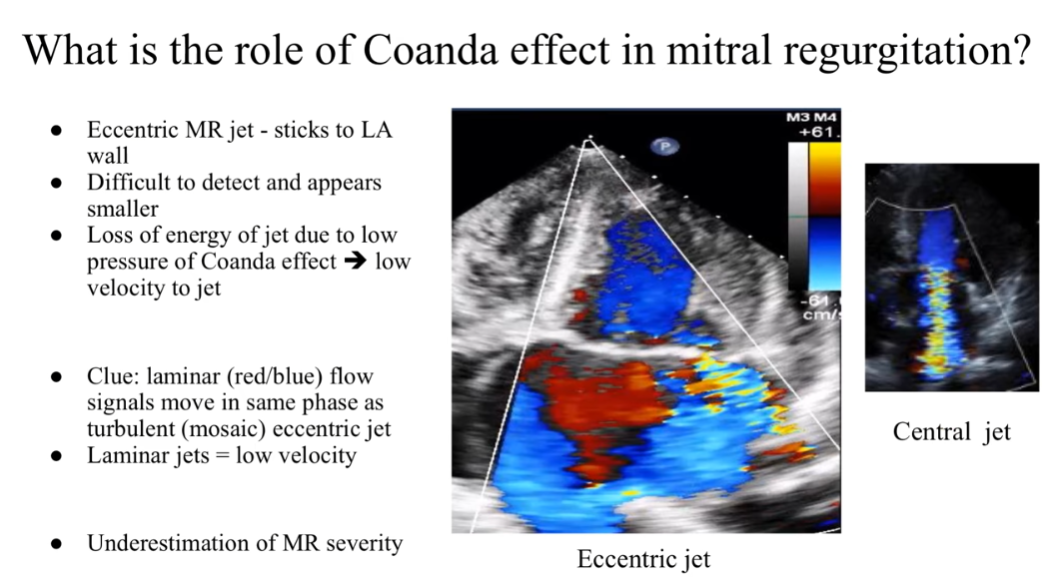
\includegraphics[keepaspectratio]{images/coandarole.png}}
\pandocbounded{
\includegraphics[keepaspectratio]{images/coanda.gif}}

\section{Vuodon mekanismi}\label{vuodon-mekanismi}

Mitraalivuodon mekanismin arvioiminen on tärkeä osa ultraäänitutkimusta ja mekanismi ohjaa merkittävästi mahdollisia hoitovaihtoehtoja. Mekanismit jaetaan Carpentierin luokituksessa kolmeen pääluokkaan sen mukaan onko läppäpurjeiden liike normaalia (I), liiallista (II) vai rajoittunutta (IIIa ja IIIb). Arvioiminen on mahdollista transtorakaalisesti, mutta TEE tietysti mahdollistaa paljon paremman läppävisualisaation.

\pandocbounded{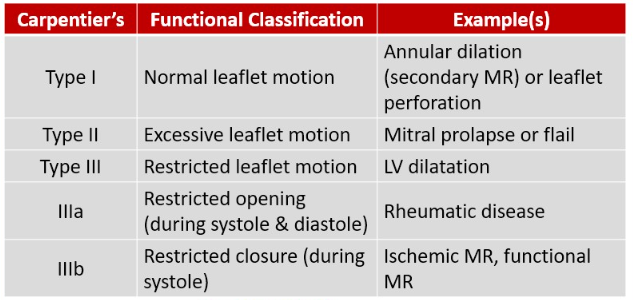
\includegraphics[keepaspectratio]{images/carpentiercardioserv.png}}
\pandocbounded{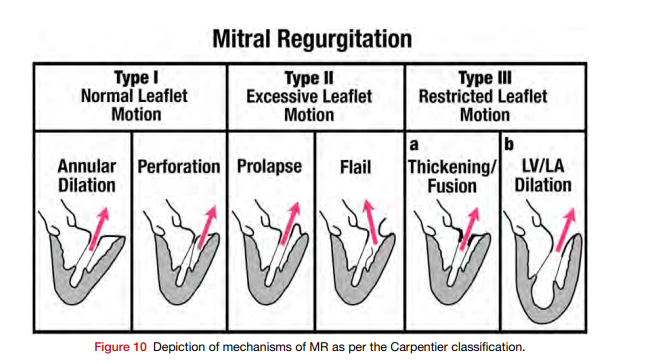
\includegraphics[keepaspectratio]{images/asecarpentier.png}}
\pandocbounded{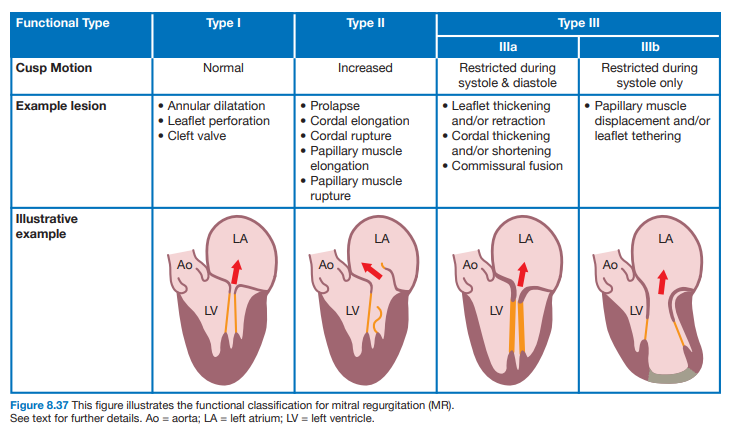
\includegraphics[keepaspectratio]{images/mrcarpentier.png}}

\subsection{Carpentier I}\label{carpentier-i}

Luokan I vuodossa läppäpurjeet liikkuvat aivan kuten kuuluukin, mutta läpässä on silti reikä tai vuoto jostain muusta syystä. Vuoto johtuu yleensä siitä, että läppäpurjeet eivät ylety kohtaamaan toisiaan keskellä (koaptaatio on heikkoa).

Tyypillisin syy on läppärenkaan laajentuma (annuluksen dilataatio) johtuen eteisen laajentumasta. Dilataatio vetää purjeita kauemmas toisistaan ja estää niiden koaptaation systolessa -\textgreater{} vuoto, joka on yleensä sentraalinen.

Toinen syy on läppäperforaatio esimerkiksi endokardiitista johtuen (yleensä anteriorinen purje); tämä näkyisi vuotona ``purjeen läpi''. Läpässä voi olla myös synnynnäinen halkio (cleft), joka aiheuttaa läppään vuodon.

Tässä on videoita Carpentier I -luokan vuodoista:

\pandocbounded{\includegraphics[keepaspectratio]{images/c1dilatation.gif}}

TEE:ssä vasemman eteisen laajentuman aiheuttama annulusdilataatio -\textgreater{} sentraalinen vuoto

\pandocbounded{\includegraphics[keepaspectratio]{images/mrperf.gif}}

Tässä on anteriorisen purjeen perforaatio, joka näkyy vuotona suoraan purjeen läpi (näkyy myös aorttavuotoa)

\pandocbounded{\includegraphics[keepaspectratio]{images/perfkohta.gif}}

Tässä saman perforaation kohta piirrettynä

\subsection{Carpentier II}\label{carpentier-ii}

Tyypin II vuodossa läppäpurje tai sen osa pääsee liikahtamaan liikaa eli se pullottaa vasemman eteisen puolelle systolen aikana, minkä vuoksi läpän reunat eivät tiivisty vastakkain, vaan veri pääsee suihkuamaan ohi.

Tyypillisin syy on mitraaliläpän prolapsi (MVP), joka on yleisin mitraalivuodon syy ylipäätään. Mitraaliläpän prolapsi johtuu läpän myksoidista degeneraatiosta, mikä tekee läpästä pehmeän ja purjeet pääsevät pullottamaan eteiseen annulustason toiselle puolelle (joissain lähteissä rajana \textgreater2mm). Etiologia ei ole selvää, mutta joskus voi olla geneettisiä sairauksia taustalla (esim. Marfanin tai Ehlers-Danlosin oireyhtymät). MVP:stä käytetään usein myös nimitystä Barlowin oireyhtymä.

Luokkaan kuluu myös jännerihmarepeämät (kordaruptuurat) ja papillaarilihasrepeämät, jotka voivat aiheuttaa vaikeaa ja akuuttia mitraalivuotoa ns. flail leafletin (vapaasti heiluva läppäprolapsi) takia.

\pandocbounded{\includegraphics[keepaspectratio]{images/mvpmad.gif}}

Tässä näkyy mitraaliläpän purjeiden pullistuminen eteiseen (mitraaliläpän prolapsi, MVP). Samalla näkyy myös mitraaliannuluksen disjunktio (MAD), joka on rakenteellinen häiriö, jossa mitraaliläpän posteriorisen purjeen saranakohta erkanee kammion myokardiumista (käytännössä siis purje kiinnittyy korkeammalle eteiseen). MAD on usein yhteydessä prolapsiin (ja voi pahentaa sitä, koska stabiilia kammioankkurointia ei ole ja annuluksen lisääntynyt liike aiheuttaa lisääntynyttä stressiä purjeisiin ja jännerihmoihin) ja on yleensä synnynnäinen ongelma. Sen aiheuttama mekaaninen stressi myös ärsyttää sydänlihasta ja johtaa myös paikalliseen lihasvaurioon (ja lopulta arpeutumiseen, joka voidaan nähdä sydämen MRI:ssä) -\textgreater{} alttius rytmihäiriöille on korkeampi (arytmogeeninen mitraaliläpän prolapsi, AVMP).

Alla vielä MAD:sta havainnollistavampi kuva

\pandocbounded{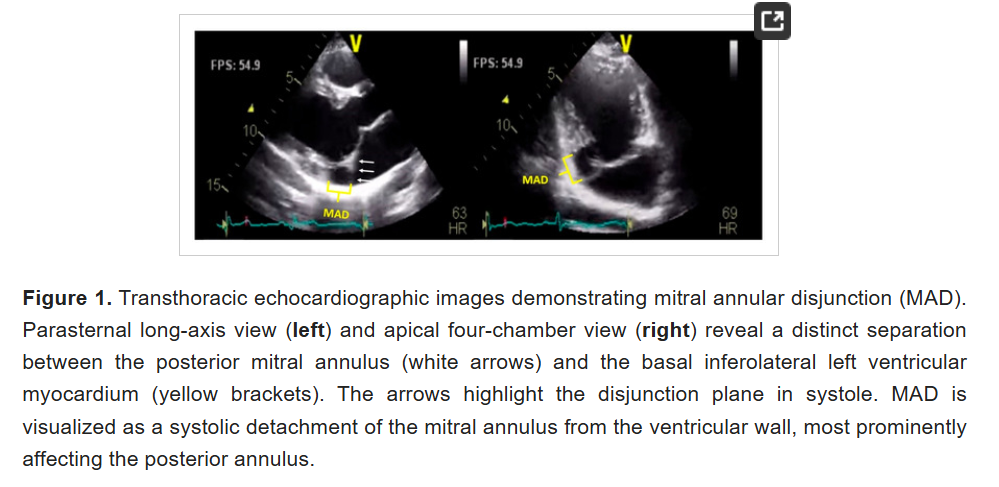
\includegraphics[keepaspectratio]{images/mad.png}}

\subsection{Carpentier IIIa}\label{carpentier-iiia}

Luokka III eli rajoittunut liike jaetaan kahteen alaluokkaan sen mukaan, missä vaiheessa liike on rajoittunutta. Tyyppi IIIa kuvastaa rajoittunutta liikettä sekä systolessa että diastolessa. Läppäpurjeet ja niiden alla olevat jännerihmat ovat kauttaaltaan paksuntuneet, jäykistyneet ja usein kasvaneet toisiinsa kiinni. Läppä ei aukea kunnolla (aiheuttaa myös stenoosia) eikä mene kunnolla kiinni. Tyypillisin syy klassisesti on reumakuumeen aiheuttama läppäsairaus (krooninen reumaattinen sydänsairaus), mutta sen yleisyys on vähentynyt Suomessa merkittävästi ja nykyään ikääntymisen aiheuttama kalsifikaatio on yleisempää. Muut syyt ovat harvinaisia, mutta niitä ovat esim. tietyt lääkkeet (esim. vanhat fenfluramiinia sisältäneet laihdutuslääkkeet), säteily ja systeemiset autoimmuunisairaudet.

\pandocbounded{\includegraphics[keepaspectratio]{images/mrstenreg.gif}}
\pandocbounded{\includegraphics[keepaspectratio]{images/mvcalc.gif}}

\subsection{Carpentier IIIb}\label{carpentier-iiib}

Tyypin IIIb-vuodossa liike on rajoittunut vain systolessa eli sulkeutumisvaiheessa. Läppäpurjeet itsessään voivat olla aivan terveen näköiset, mutta niitä vedetään alaspäin kammion pohjaa kohti (ilmiötä kutsutaan nimellä tethering). Kun kammion seinämä venyy ulospäin, papillaarilihakset siirtyvät ja jännelangat vetävät läppää tiukasti alas, jolloin se ei pääse nousemaan ylös sulkeutuakseen. Tyypillisimpiä syitä ovat infarktin jälkitila (infarktialueen seinämä pullistuu) tai dilatoiva kardiomyopatia.

Tyypin I ja IIIb Carpentier eroavat siten, että tyypissä I läppäliike ei ole rajoittunutta ja purjeet nousevat ylös läppätasoon asti. Ne vain eivät yletä sulkemaan aluetta johtuen eteisen dilataatiosta. Carpentier IIIb:ssa purjeiden liike on rajoittunut ja ne jäävät kammion puolelle johtuen pääasiassa vasemman kammion dilataatiosta. Nykyään käytetään usein termejä \textbf{atrial MR} (annulusdilataatiosta johtuva koaptaatiovaje = carpentier I) ja \textbf{ventricular MR} (kammiolaajentumisesta johtuva koaptaatiovaje = carpentier IIIb)

\pandocbounded{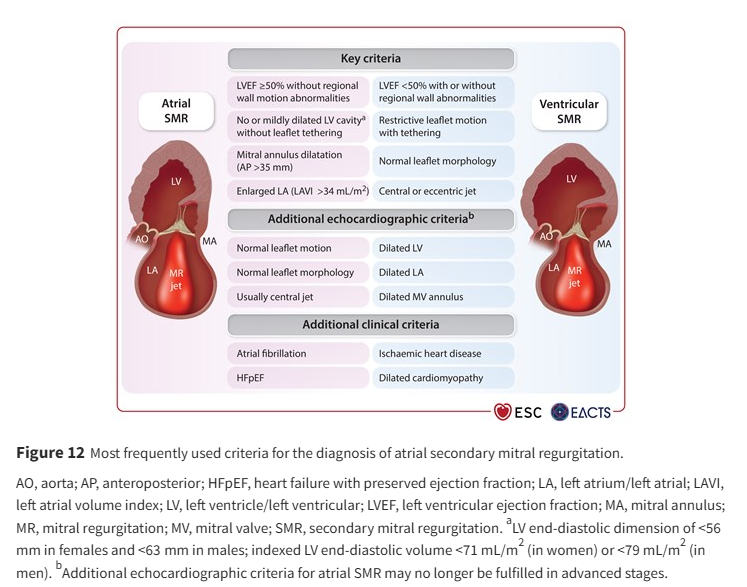
\includegraphics[keepaspectratio]{images/atrialvsventricularmr.png}}

Tässä videossa on tyypillinen tyypin IIIb mitraaliläpän funktio, joka aiheuttaisi funktionaalista mitraalivuotoa. Papillaarilihasten siirtyminen on johtanut jännerihmojen jännittyneisyyteen, mikä vetää anteriorista purjetta lentävän lokin muotoiseksi (``seagull sign''). Posteriorista purjetta vedetään vahvasti seinämää pohti ja se onkin tässä pääasiallinen koaptaatiovajeen ja vuodon aiheuttaja. Joskus kuvaaja voi mennä harhaan ja luulla tätä tilaa anteriorisen purjeen prolapsiksi, jos vain katsoo anteriorisen ja posteriorisen purjeen suhdetta toisiinsa, mutta tulee huomata, että purje ei pullistu kammioon (ei ylitä annulustasoa eteisen puolelle).

\pandocbounded{\includegraphics[keepaspectratio]{images/mvpnot.gif}}

\section{Vuodon gradeeraus}\label{vuodon-gradeeraus}

Mitraalivuodon gradeeraus voidaan toteuttaa monella eri metodilla ja onkin yleensä hyvä hyödyntää monia eri tekniikoita, jotta saa paremmin hajautettua arvion eikä se nojaa yhteen ainoaan arvoon. Vuotoaukon pinta-alan (EROA) laskeminen on usein kuitenkin paras yksittäinen mitraalivuodon vaikeusasteen määritysmenetelmä. Myös mm. vena contractan leveyttä voi käyttää. Molempien luotettavuus usein laskee toiminnallisessa vuodossa epäsymmetrisen vuotoaukon vuoksi.

\subsection{Vena contractan leveys (VCW)}\label{vena-contractan-leveys-vcw}

Ennen EROA:n laskemista yleensä kyllä mitataan vuodon kaulakin (vena contractan leveys), koska sen merkkaaminen auttaa taas PISA:n säteen mittaamisessa (lisää tästä kohta). Vuodon kaulan mittaaminen on myös hyvä ja nopea tapa saada arvio vuodon vaikeudesta.

Vuodon kaula kannattaa mitata niistä projektioista, joista kaikki vuodon kolme anatomista osaa ovat nähtävissä. Nyquistin rajan (aliasing velocity) tulisi olla yleensä standardi (unshifted) eli n.~50-60(-70)m/s. Mitatessa kannattaa zoomata lähelle vuotoa.

Mittaus suoritetaan silloin, kun vuotosuihku on suurimmillaan eli mitraalivuodon suhteen yleensä keskisystolessa (tosin prolapsissa maksimivuoto on usein myöhäissystolessa). Itse mitta on siis vuodon kapein kohta, jonka voi visualisoida olevan juuri pisan puolikaaren alapuolella. Tämän voi mitata ihan vain caliperilla, koska tästä ei tehdä itse ultraäänilaitteen sisällä jatkolaskelmia.

Kannattaa ottaa keskiarvo kahdesta tai kolmesta lyönnistä ja myös kahdesta ortogonaalisesta suunnasta (yleensä siis PLAX ja A4C).

\pandocbounded{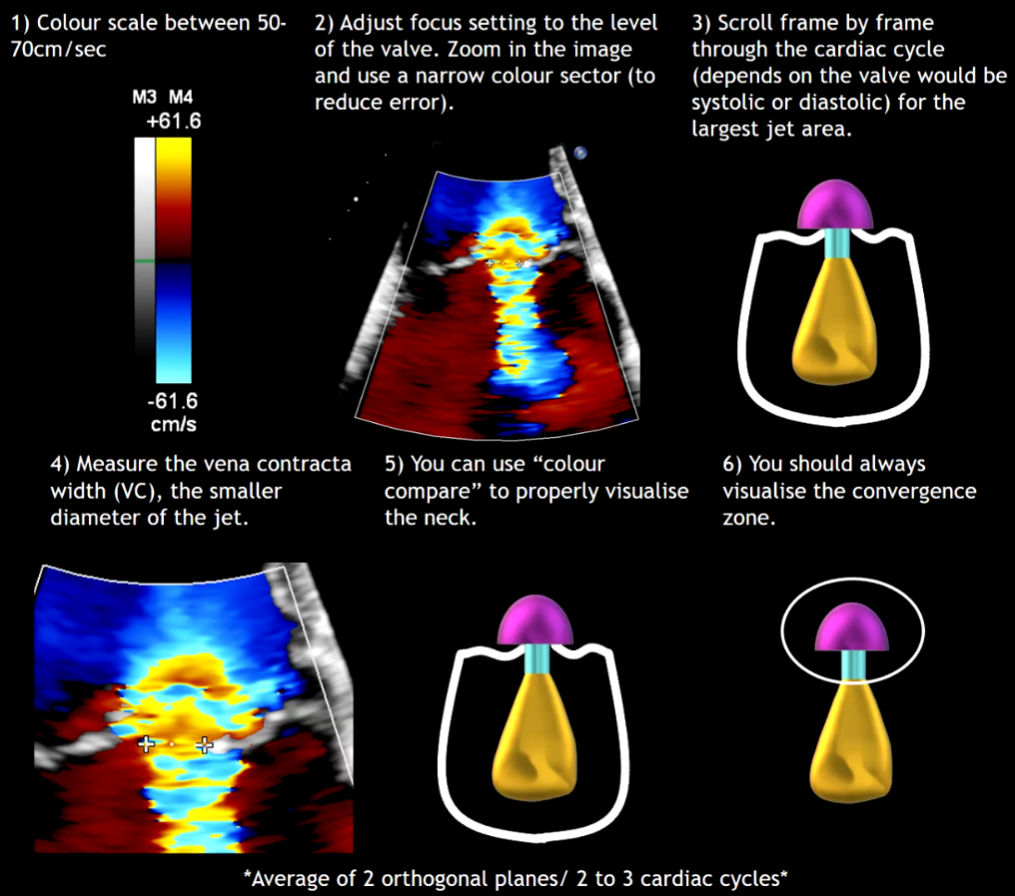
\includegraphics[keepaspectratio]{images/venacontractawidth.png}}

\subsection{EROA}\label{eroa}

EROA eli Effective Regurgitant Orifice Area tarkoittaa käytännössä vuotoaukon pinta-alaa; ``efektiivinen'' -osa vain tulee siitä, että nestefysiikan takia itse vuotavan veren pinta-ala on pienempi kuin anatomisen vuotoaukon. EROA ajatellaan hydrodynaamisesti samaksi kuin vena contractan kautta lasketun ympyrän pinta-ala.

\textbf{EROA lasketaan kahdesta arvosta: PISA:n säde ja vuotosuihkun maksimaalinen nopeus.}

\subsubsection{PISA:n säde (PISA radius)}\label{pisan-suxe4de-pisa-radius}

PISA:n säde mitataan EROA:sta eli käytännössä vuodon kaulasta PISA:n värireunaan (point of colour aliasing).

Aliasing eli käänteisilmiö on artefakta, jota voi tapahtua doppler-UÄ:ssä, kun virtauksen nopeus ylittää Nyquistin rajan. Nyquistin raja on se korkein virtausnopeus, jonka ultraäänilaite pystyy vielä mittaamaan oikein. Mittaaminen perustuu siihen, että laite lähettää ultraäänipulsseja tietyllä taajuudella (PRF, Pulse Repetition Frequency). Jotta laite pystyisi laskemaan veren virtausnopeuden oikein, sen täytyy ``ottaa näytteitä'' (eli lähettää pulsseja) vähintään kaksi kertaa nopeammin kuin mikä on mitattavan virtausliikkeen aiheuttama taajuusmuutos. Nyquistin raja on aina tasan puolet laitteen pulssintoistotaajuudesta (PRF) eli Nyquistin raja = PRF/2.

Käänteisilmiö voidaan havaita dopplerkuvauksessa niin aaltokäyristä kuin värispektridopplerissa. Väridopplerissa nopeasti virtaava veri (esimerkiksi ahtauman kohdalla) muuttuu yhtäkkiä yksisuuntaisesta väristä (esim. kirkkaanpunainen) vastakkaiseksi väriksi (siniseksi), ja värit ikään kuin sekoittuvat mosaiikkimaiseksi pyörteeksi (myös siis turbulenssista johtuen). PW-dopplerissa doppler-käyrän huippu taas voi leikkautua poikki asteikon yläreunasta ja ilmestyä näkyviin asteikon pohjalle (ikään kuin virtaus olisi muuttanut suuntaa).

Oikean elämän esimerkki aliasingista on autojen renkaat elokuvissa. Kun auto kiihydttää, kameran kuvanopeus (frames per second) ei enää riitä tallentamaan pyörän liikettä oikein. Pyörä voi ehtiä pyörähtämään lähes täyden kierroksen kahden kuvan välissä ja silmille syntyy illuusio, että pyörä pyöriikin taaksepäin (jos ehtisi pyörähtämään täydellisen kierroksen, niin rengas vaikuttaisi olevan paikallaan).

\begin{center}\rule{0.5\linewidth}{0.5pt}\end{center}

Mitraalivuodon PISA-sädettä mitatessa Nyquistin raja tulee asettaa tasolle 30-40 cm/s vuodon suuntaan (eli siis jos vuoto on negatiivinen, niin silloin nyquist esim. -38.5 cm/s), koska se auttaa rajaamaan konvergenssialuetta ja tekemään siitä selkeälukuisen. Standardirajoilla (n.~60-70 cm/s) aliasing tapahtuu liian lähellä pientä vuotoaukkoa; tällaista pientä aluetta on vaikea mitata ja koska EROA:n laskelmissa käytetään pisa-säteen neliötä, on pienikin mittausvirhe suuri lopputuloksen kannalta. Pakottamalla aliasingin tapahtuvan aikaisemmin, tehdään PISA-säteestä suurempi ja siten helpotetaan mittausta.

Mittaus suoritetaan siis näin (kannattaa olla zoomattuna, niin on helpompaa ja tarkempaa):

0 - Mittaa vuodon kaula (Nyquist 50-60 cm/s)

1 - Vaihda Nyquist tasolle 30-40cm/s vuodon suuntaan

2 - Etsi kohta, jolloin vuotovirtaus on nopeinta (VMax, yleensä keski- tai myöhäissystolessa); tämä siis vastaa stabiileinta (ei siis sinänsä suurinta; liian aikaisin mitattuna PISA voidaan mitata liian isona) hemisfeeristä PISA-puolikaarta

3 - PISA:n säde on alue ensimmäisestä värimuutoksesta (yleensä siis sinisestä keltaiseksi, jos vuoto poispäin anturista) vena contractaan

\pandocbounded{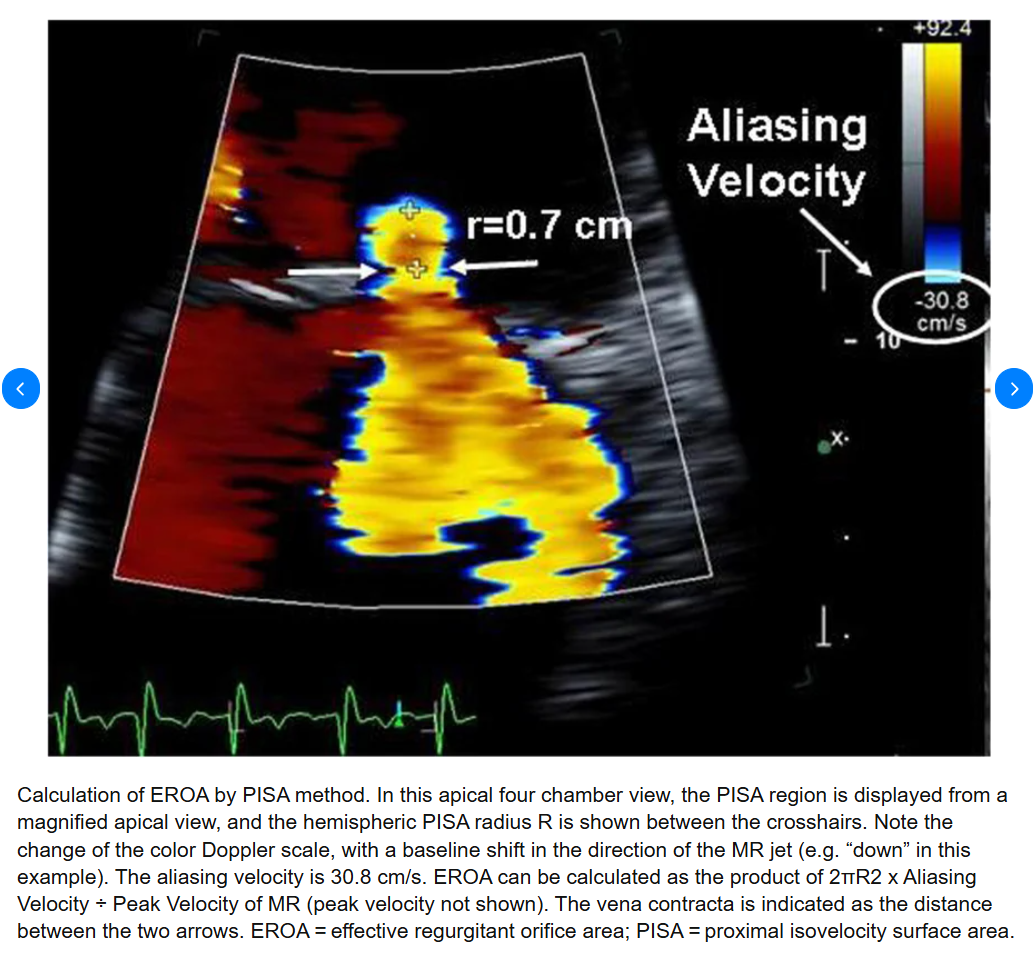
\includegraphics[keepaspectratio]{images/pisaradius.png}}
\pandocbounded{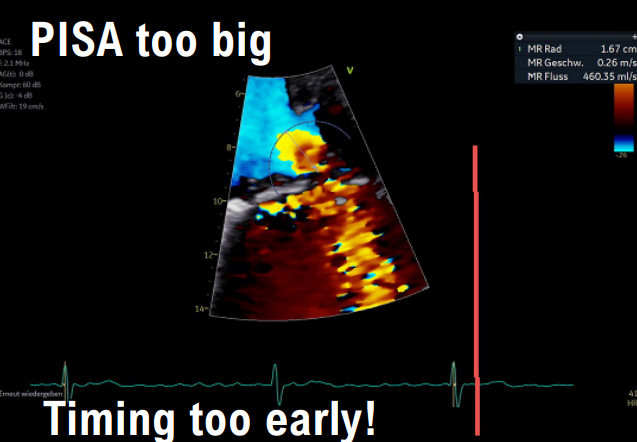
\includegraphics[keepaspectratio]{images/pisatiming.png}}

\subsubsection{CW Dopplerilla vuodon nopeus (ja VTI)}\label{cw-dopplerilla-vuodon-nopeus-ja-vti}

Periaatteessa EROA voidaan laskea pelkästään vuodon maksiminopeudesta (VMax) eikä vuodon nopeus-aika-integraalia (VTI) tarvitse piirtää, mutta VTI:n mittaaminen mahdollistaa samalla myös vuodon tilavuuden arvioimisen, mikä taas auttaa vuodon gradeerauksessa sekä sen mittausluotettavuuden arvioinnissa. Kannattaakin siis rutiinisti piirtää vuodon VTI.

EROA lasketaan (kone laskee automaattisesti tai voi halutessaan laskea nettilaskureilla), kun tiedetään vuotoaukon saama virtaama (flow rate (ml/s)) ja vuodon maksiminopeus. Tämä perustuu siihen, että kaikki veri, joka virtaa PISA-puolipallon läpi, on samaa verta, joka puristuu myöhemmin läpän vuotoaukon läpi. EROA siis lasketaan kaavasta:

\pandocbounded{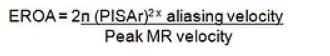
\includegraphics[keepaspectratio]{images/eroaequation.png}}

Yhtälön osoittaja siis laskee vuodon virtaaman eli sen, kuinka paljon verta (millilitroina sekunnissa) virtaa kohti vuotokohtaa. 2πr\^{}2 on PISA-puolipallon pinta-ala, joka lasketaan, kun tiedetään PISA-radius. Aliasing velocity on asettamasi Nyquistin raja, joka kuvastaa sitä, että puolipallon pinnalla kaikki veri liikkuu sillä nopeudella. Voi siis ajatella näin: Jos tietää, kuinka leveä paloletku on ja kuinka lujaa vesi siinä virtaa (Nyquist limit), tietää montako litraa vettä letkusta tulee sekunnissa.

Kun tämä määrä vettä (nyt sydämessä verta) suppenee ja puristuu systolessa läpän pienen vuotoreiän läpi, sen virtausnopeus lähtee nousemaan. Koska verta ei katoa minnekkään PISA:n ja vuotoaukon välillä (jatkuvuusyhtälö), niin virtaus PISA-puolipallossa on sama kuin virtaus vuotoaukossa. Täten voi ajatella, että EROA (vuotoaukon pinta-ala) x VMax = PISA:n virtaama. Tästä vain ratkaisemalla EROA saadaan yllä oleva kaava.

\begin{center}\rule{0.5\linewidth}{0.5pt}\end{center}

VTI:n mittaaminen on myös tärkeää vuodon gradeerauksessa ja on vain seuraava laskutoimitus EROA-kaavassa. Kun tiedetään vuotoaukon pinta-ala (EROA), niin voidaan laskea myös vuodon tilavuus, jos tiedetään vuodon muodostaman sylinterin pituus. Kuten käytiin jo aorttastenoosin yhteydessä läpi, niin VTI (velocity time integral; aika kertaa nopeus = etäisyys) kuvastaa sitä matkaa, jonka verisolut kulkevat yhden sydämenlyönnin aikana. Kun tiedetään vuodon alun pinta-ala ja tiedetään ``vuodon kulkema etäisyys'', niin tiedetään vuodon tilavuus. Voi siis ajatella ruiskua: EROA on ruiskun sylinterin poikkipinta-ala. VTI puolestaan on se matka, jonka verran ruiskun mäntää painetaan sisään yhden lyönnin aikana. Pinta-ala kertaa matka kertoo, kuinka monta millilitraa nestettä ruiskusta pursuaa ulos.

\pandocbounded{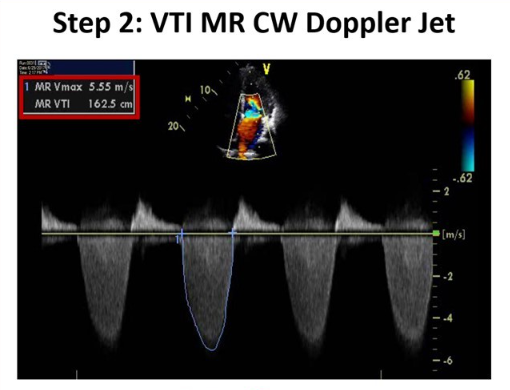
\includegraphics[keepaspectratio]{images/mrvti.png}}
\pandocbounded{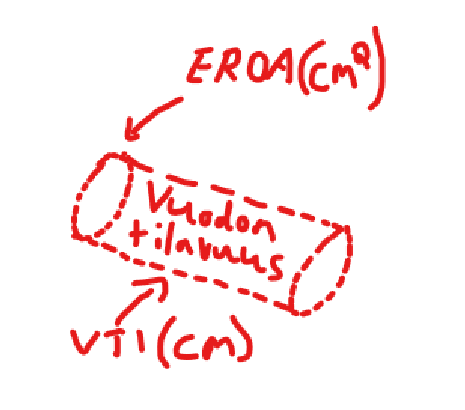
\includegraphics[keepaspectratio]{images/eroavtivol.png}}
\pandocbounded{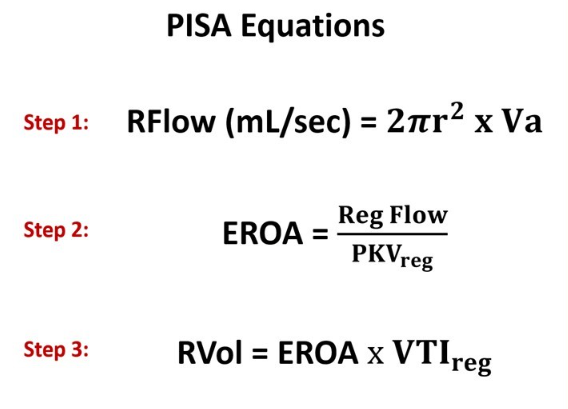
\includegraphics[keepaspectratio]{images/pisaequations.png}}

\subsection{Muut gradeeraustavat}\label{muut-gradeeraustavat}

Usein jo pelkästään EROA:lla ja vuodon tilavuudella saadaan hyvä arvio vuodon vaikeusasteesta ja nämä ovatkin käytetyimmät arvot gradeerauksessa. Kuitenkin on todella järkevää vahvistaa arviota multiparametrisesti eli keräämällä muutakin dataa (niin kvalitatiivisia, semi-kvantitatiivisia ja kvantitatiivisia), kuten vena contractan leveys, RF\%, keuhkolaskimoiden virtaus, LA:n / LV:n koko, diastoliset mitraalivirtaukset ja keuhkovaltimopaine.

Vena contractan leveys onkin jo käyty läpi: se käytännössä siis kuvastaa EROA:a (ainakin yleensä rakenteellisessa vuodossa). Miten nämä muut sitten soveltuvat mitraalivuodon gradeeraukseen?

\subsubsection{RF\%}\label{rf}

Vuodon osuus (regurgitant fraction, RF\%) lasketaan vuodon tilavuuden ja diastolisen mitraalivirtauksen tilavuuden suhteena. Vuodon tilavuuden voi tässä yhteydessä periaatteessa laskea jo aikaisemmin osoitetulla tavalla vuodon VTI:n ja EROA:n kautta, mutta vuodon tilavuuden voi myös arvioida toisella tavalla. Tämä metodi myös mahdollistaa EROA:n laskemisen ilman PISA:a (ja toimii taas yhtenä tapana saada luotettavampaa dataa multiparametrisesti).

Voidaan siis mitata aikaisemmin opetettuun tapaan vasemman kammion systeeminen iskutilavuus (LVOT SV; aortic outflow). Sitten jos lasketaan myös mitraaliläpän iskutilavuus eli se määrä verta, jota mitraaliläpän läpi kulkee diastolessa kammioon (MV SV; mitral inflow), niin saadaan näiden erotuksesta laskettua mitraalivuodon tilavuus (MV RV = MV SV - LVOT SV).

Mitraaliläpän iskutilavuus saadaan laskettua samalla periaatteella kuin LVOT SV: mitataan aluksi läpän annuluksen läpimitta ja sen jälkeen piirretään sen läpi virtaavan veren VTI.

Läpän annulus mitataan apikaalisessa nelilokerokuvassa (tai kaksilokerokuvassa; aorttaa ei kuitenkaan saisi siis näkyä joten ei 3- tai 5-lokerokuvaa) keskidiastolessa (mitraaliläppä auki).

Mitral inflow mitataan samalla tavalla kuin diastoliikassa, mutta tällä kertaa piirretään E- ja A-aaltojen muodostama VTI.

Eli siis siirretään sample gate mitraaliläpän kärkien kohdalle ja mitataan pulssiaaltodoppleri (PW).

Sitten tulee piirtää nopeuskäyrän pinta-ala (MV VTI); tietysti jos on vain E-aalto esillä, niin sitten vain se piirretään

MV SV lasketaan kaavasta π × d²/4 × MV VTI = 0.785 × d² × MV VTI (useimmat koneet toteuttavat laskun suoraan, jos on tehnyt calc:n kautta mittaukset).

\begin{center}\rule{0.5\linewidth}{0.5pt}\end{center}

Kun on myös mitannut LVOT VTI:n ja LVOT Diam kautta aorttaan kulkevan stroke volumen (LVOT SV), niin voi arvioida, että se veri, joka ei kulje systolessa aorttaan, kulkee mitraaliläpän läpi vuotona. Täten MV SV - LVOT SV on MV RV (regurgitant volume).

Tästä voi sitten laskea vuodon fraktion eli RF = vuodon tilavuus / vasemman kammion totaali-iskutilavuus = (Mitraaliläpän iskutilavuus - systeeminen iskutilavuus) / mitraaliläpän iskutilavuus

RF = (MV SV - LVOT SV) / MV SV

\begin{center}\rule{0.5\linewidth}{0.5pt}\end{center}

Samalla voidaan taas laskea EROA, mutta tällä kertaa ilman PISA:n mittaamista. Tätä tulosta voi sitten verrata PISA-metodilla saatuun tulokseen.

EROA = MV RV / MR TVI = mitraalivuodon tilavuus / mitraalivuodon TVI

Eli siis tulee mitata lisäksi vielä vuodon VTI. Kun tietää vuodon tilavuuden (juuri laskettu MV SV - LVOT SV) ja vuodon VTI:n (vuotosylinterin pituuden), voi tästä laskea vuotosylinterin pohjan pinta-alan eli vuotoaukon koon.

\pandocbounded{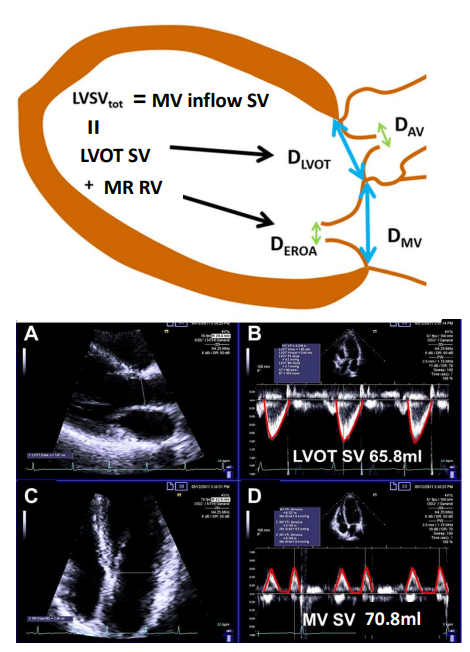
\includegraphics[keepaspectratio]{images/picturemvsv.png}}
\pandocbounded{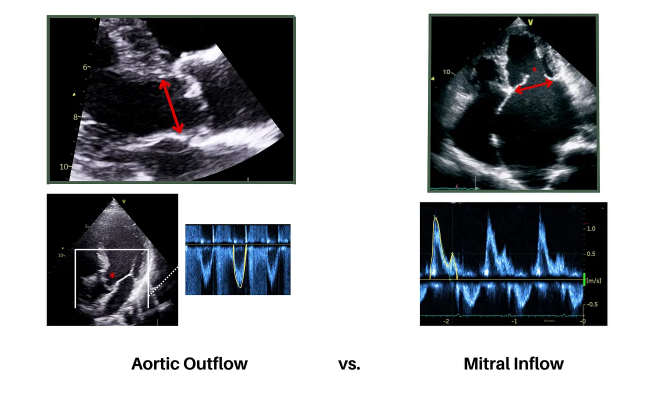
\includegraphics[keepaspectratio]{images/aorticoutflowvsmitralinflow.png}}
\pandocbounded{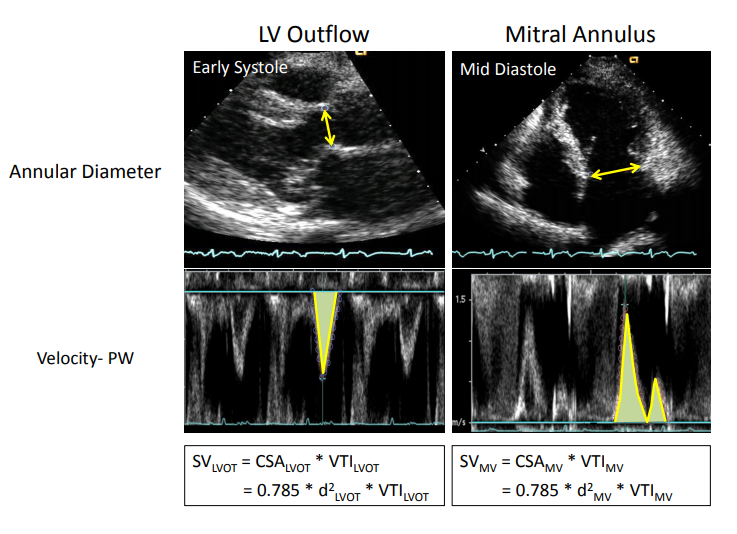
\includegraphics[keepaspectratio]{images/mitralsv.png}}
\pandocbounded{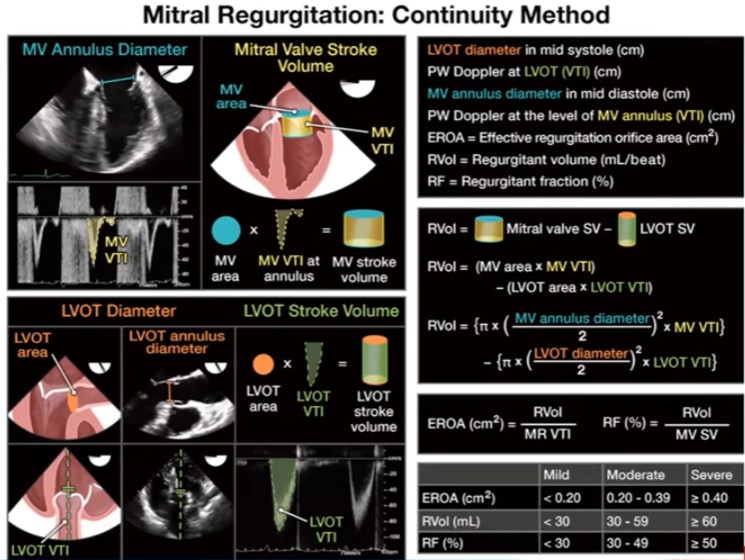
\includegraphics[keepaspectratio]{images/mrrv1.png}}
\pandocbounded{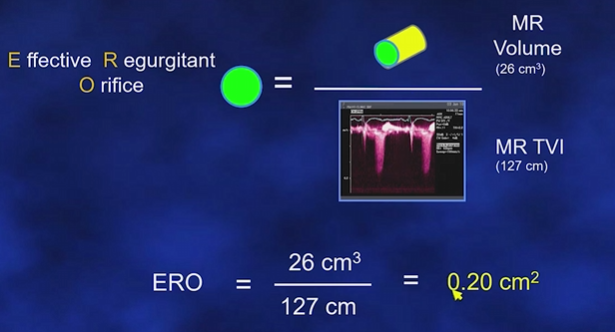
\includegraphics[keepaspectratio]{images/eronottvi.png}}

\subsubsection{Diastoliset mitraalivirtaukset}\label{diastoliset-mitraalivirtaukset}

Kannattaa myös arvioida diastoliikkaa; erityisesti mitraaliläpän diastolisten virtausten nopeuksia.

Mitraaliläpän alkudiastolinen virtausnopeus (E-aalto) kiihtyy vääjäämättä merkittävässä mitraalivuodossa, koska vuototilavuuden verran ``ylimääräistä'' verta palaa seuraavan diastolen aikana takaisin kammioon ja diastolen alussa paine-ero lokeroiden välillä on suurentunut. Yleensä E-aalto on ≧ 1.2 m/s (tosin nopeita E-aaltoja voidaan nähdä myös mm. diastolisessa vajaatoiminnassa; ei siis ole täysin spesifinen). E/A-suhde myös tietysti tästä johtuen laskee ja dominantti A-aalto poissulkee vaikean mitraalivuodon (ei tosin pysty hyödyntämään tätä tietoa, jos potilas on eteisvärinässä, koska A-aaltoja ei ole).

\begin{center}\rule{0.5\linewidth}{0.5pt}\end{center}

Samalla voidaan myös mitata E-aallon puoliintumisaika ja deceleration time ja näistä vielä mitraaliläpän avautumispinta-ala (MVA). Tästä enemmän mitraalistenoosin yhteydessä.

\subsubsection{Keuhkolaskimovirtaukset}\label{keuhkolaskimovirtaukset-2}

Keuhkolaskimoiden visualisoimisesta ja myös niiden virtausten mittaamisesta ollaan jo puhuttu. Keuhkolaskimovirtausten mittausta voi myös hyödyntää mitraalivuodon vaikeusasteen arvioimisessa.

Nopea kertaus keuhkolaskimoista ja niiden virtausaalloista:

Mittaukset suoritetaan yleensä apikaalisesta nelilokerokuvasta ja yleisimmin kuvannetaan ylempää oikeaa keuhkolaskimoa (RUVP). Pulssiaallot mitataan n.~0.5-2cm proksimaalisesti laskimon junktiosta vasemman eteisen kanssa.

PW-dopplerin piirtämä virtauskäyrä koostuu S-, D- ja Ar-aalloista; S-aalto (joskus voi erottaa S1 ja S2) syntyy eteisen täyttyessä kammiosystolen aikana. D-aalto syntyy keuhkolaskimoveren virratessa eteiseen eteisen tyhjentyessä aikaisdiastolessa. Ar-aalto syntyy eteissystolessa eteisen puristaessa loputkin veret eteisestä kammioon (supistumisen aiheuttama paine aiheuttaa hieman retrogradista virtausta keuhkolaskimoon).

\begin{center}\rule{0.5\linewidth}{0.5pt}\end{center}

Mitraalivuodon pahentuessa voidaan todeta progressiivista S-aallon amplitudin laskua ja D-aallon korostumista. Vaikeassa mitraalivuodossa tyypillinen löydös on S-aallon kääntyminen (SR, systolic reversal).

S-aallon heikentyminen johtuu siitä, että mitraalivuoto on systolinen tapahtuma. Normaalisti systolessa verta virtaa vapaasti keuhkolaskimoista vasempaan eteiseen, mutta mitraalivuodossa eteiseen suihkuaa kuitenkin samanaikaisesti verta suurella paineella vasemmasta kammiosta. Tämä vuotosuihku nostaa eteisen painetta nopeasti, mikä luo vastapaineen keuhkolaskimoista tulevalle normaalille virtaukselle. Koska virtaus edellyttää paine-eroa (korkeammasta matalampaan), vastapaine jarruttaa eteenpäin suuntautuvaa S-aaltoa, jolloin se madaltuu.

D-aalto taas korostuu, koska diastolen alkaessa eteinen on ylitäyttynyt kammiosta vuotaneen veren takia. Kun mitraaliläppä vihdoin aukeaa, tämä korkeapaineinen verimäärä purkautuu paineella takaisin vasempaan kammioon. Tämän virtauksen aiheuttama tilavuusmuutos ja imu vetävät laskimoista nopeasti suuren määrän uutta verta, mikä näkyy korkeana ja terävänä D-aaltona.

Kun S-aalto kääntyy nollatason alapuolelle (systolic flow reversal), se on vaikea-asteisen mitraalivuodon klassinen tunnusmerkki. Tässä tilanteessa regurgitaatiosuihku on niin voimakas ja volyymi niin suuri, että se ei enää pelkästään jarruta keuhkolaskimoista tulevaa verta, vaan vuotavan veren paine ylittää keuhkolaskimoiden paineen kokonaan. Tämän seurauksena veri iskeytyy eteisen läpi ja työntyy fyysisesti taaksepäin keuhkolaskimoihin.

Kääntyminen tapahtuu klassisesti keski- tai myöhäissystolessa, jonka takia S1-aalto voi vielä olla todettavissa (tai olla poissa), vaikka S2 olisikin käänteinen. Holosystolinen kääntyminen on harvinaisempaa, mutta joskus todettavissa todella vaikeassa vuodossa.

\begin{center}\rule{0.5\linewidth}{0.5pt}\end{center}

On hyvä tiedostaa, että normaali keuhkolaskimovirtausprofiili ei poissulje vaikeaa mitraalivuotoa. Jos potilaan mitraalivuoto on krooninen ja kompensoitu (vasen eteinen dilatoitu ja komliantti) ja LV:n systolinen funktio on normaali, niin virtausprofiilit voivat hyvinkin olla normaaleja tai voi olla todettavissa vain S-aallon tylpistymistä.

S-aallon lasku ei myöskään ole kovinkaan spesifinen löydös mitraalivuodolle (käytännössä mikä tahansa syy LA:n paineen nousulle voi aiheuttaa S-aallon tylpistymistä) eikä siitä voi suoraan päätellä vuodon vaikeusastetta.

S-aallon kääntymistä (SR) taas pidetään vaikean mitraalivuodon suhteen epäsensitiivisenä, mutta spesifisenä löydöksenä. Kannattaakin siis vaikeaa mitraalivuotoa epäillessä mahdollisuuksien mukaan nopeasti vilkaista keuhkolaskimovirtaukset.

\pandocbounded{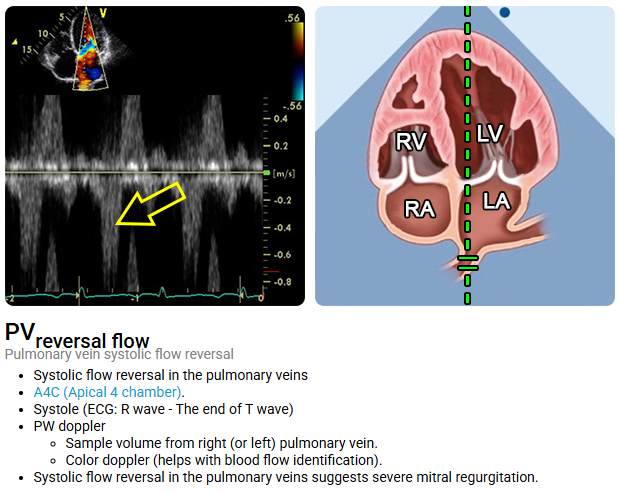
\includegraphics[keepaspectratio]{images/pvreversal.png}}
\pandocbounded{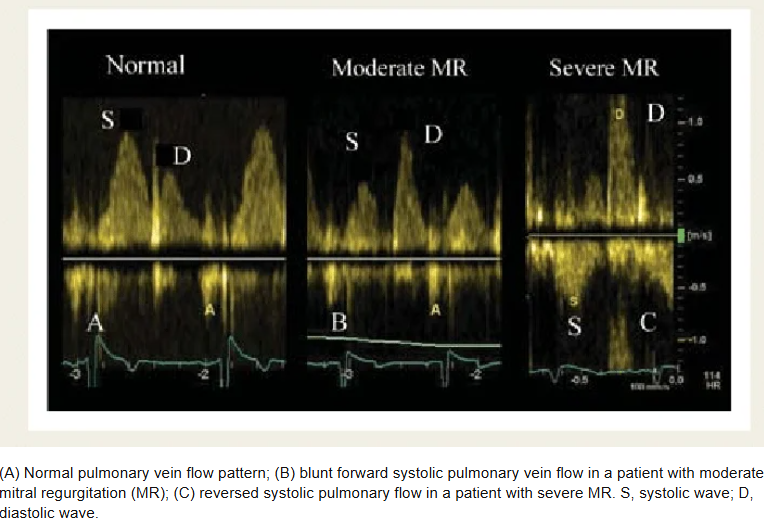
\includegraphics[keepaspectratio]{images/mrseveritypv.png}}
\pandocbounded{\includegraphics[keepaspectratio]{images/pulmonaryveinreversal.gif}}
\pandocbounded{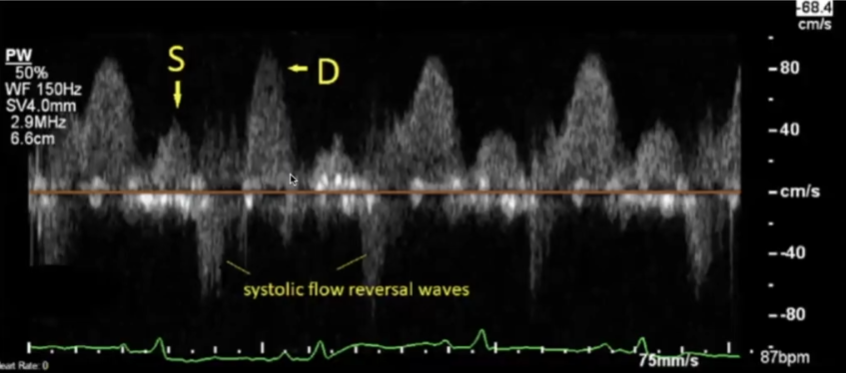
\includegraphics[keepaspectratio]{images/s1visible.png}}

\subsubsection{LA:n / LV:n koko}\label{lan-lvn-koko}

Kroonisessa mitraalivuodossa eteisen ja kammion välillä virtaava veri johtaa ennen pitkään molempien lokeroiden laajenemiseen volyymiylikuormituksen takia. LA:n ja LV:n tilavuuksien arvioimien on usein hyödyllistä mitraalivuodon vaikeusasteen ja sen vaikutuksien arvioimisessa.

Lievässä mitraalivuodossa koot voivat olla vielä normaalit, mutta ajan kuluessa ja vuodon vaikeutuessa lokerot laajentuvat etenevästi. Vaikeassa kroonisessa mitraalivuodossa vasen kammion on lähes poikkeuksetta laajentunut, tosin pienikokoisilla potilailla (varsinkin naisilla) laajentunut lokero voi vielä olla ``normaalirajojen'' sisällä, vaikka laajentumista olisikin tapahtunut merkittävästi. Tämän takia \textbf{lokeroiden koot tulisi suhteuttaa kehon pinta-alaan (body surface area, BSA);} esimerkiksi LAV:n suhde BSA:han on nimeltään LAVi eli Left Atrial Volume Index (normaali on ≤ 34ml/m2). Kammionkin koon voi suhteuttaa BSA:han, mutta usein se vain ilmoitetaan absoluuttisena kokona (normaali LVEDV miehillä on ≤ 150 ml ja naisilla ≤ 106 ml).

Akuutissakin vuodossa (esim. papillaarilihasruptuura) lokeroiden koot ovat tyypillisesti normaalikokoisia, vaikka vuoto olisikin vaikea, koska lokeroiden remodelaatiota ei ole ehtinyt tapahtumaan. Jos potilaalla on siis olevinaan muiden mittausten perusteella ``vaikea'' krooninen mitraalivuoto, mutta vasemman puolen lokeroiden mitat ovat täysin normaalit, vuodon aste on todennäköisesti yliarvioitu tai kyseessä on vasta hiljattain alkanut tilanne.

Kroonisessa vuodossa normaalit LV/LA-mitat ovat epätyypillisiä ja herättävät epäilyn siitä, onko vaikeusaste arvioitu oikein.

\begin{center}\rule{0.5\linewidth}{0.5pt}\end{center}

Mitat voi ottaa tyypilliseen tapaan. Kammiosta voi siis mitata PLAX:ssa loppudiastolisen (LVEDD, LVIDd)ja loppusystolisen (LVESD, LVIDs) läpimitan ja A4C:ssa piirtäen loppudiastolisen (LVEDV) ja loppusystolisen (LVESV) tilavuuden. Näistä kone sitten laskee automaattisesti ejektiofraktion, joka myös tulisi aina selvittää mitraalivuotopotilailta, koska EF vaikuttaa leikkauspäätökseen. Kammion loppusystolinen läpimitta on myös monissa kriteeristöissä erillinen arvioitava kriteeri leikkauksen suhteen. Eteisestä voi mitata eteisen läpimitan PLAX:ssa ja eteisen tilavuuden (LAV) voi piirtää A4C:sta; mittaukset tehdään eteisen ollessa suurimmillaan.

Ejektiofraktio siis on usein vaikeassakin vuodossa ja sen aiheuttamassa kammion dilatoivassa remodelaatiossa normaali, vaikka perfuusio eteenpäin olisikin heikkoa. Mitraalivuoto siis ryöstää suuren osan kammion pumppaamasta verestä ja tämä näkyy valheellisen korkeana ejektiofraktiona, joka yliarvioi oikeasti aorttaan kulkevan veren ja siten elimiä perfusoivan pumppaustoiminnan määrän.

Tämän takia jos vaikeaa mitraalivuotoa sairastavan potilaan EF putoaa 60\% tai sen alle, se on huono merkki ja usein merkitsee, sitä, että kammion todellinen kyky perfuusiolle eteenpäin on jo heikentynyt merkittävästi. Oireettomankin rakenteellisen vaikean mitraalivuodon leikkaushoito on siis yleensä aiheellista, kun vasemman kammion ejektiofraktio (LVEF) on \textless{} 60 \% (tai mm. jos vasemman kammion systolinen poikkimitta on ≥ 40 mm).

\pandocbounded{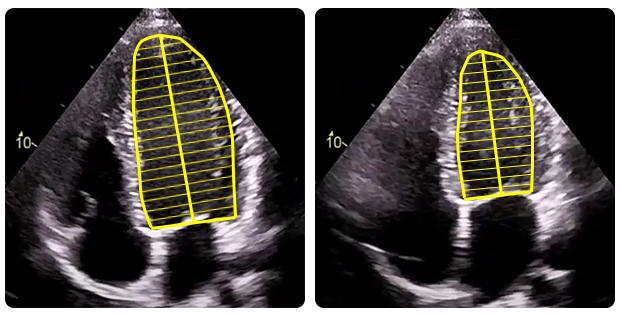
\includegraphics[keepaspectratio]{images/lvvolumes.png}}
\pandocbounded{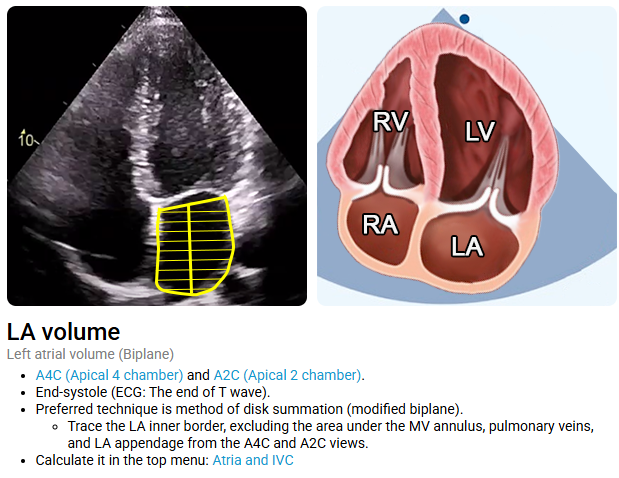
\includegraphics[keepaspectratio]{images/lavolume.png}}
\pandocbounded{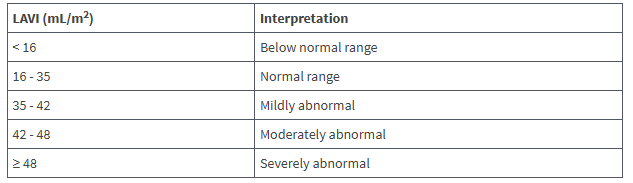
\includegraphics[keepaspectratio]{images/lavichart.png}}

\subsubsection{Vuotosuihkun pinta-ala}\label{vuotosuihkun-pinta-ala}

Kuten mainittiin aikaisemmin, niin sentraalisten vuotojen kanssa voidaan vieläkin guidelinejen mukaan hyödyntää gradeerauksessa vuotosuihkun pinta-alan ja vasemman eteisen välistä suhdetta. Painoarvoa tulokselle ei kuitenkaan tulisi antaa liikaa, koska vuotosuihkun pinta-alaan liittyy monia ongelmia.

Varsinkin eksentriset vuodot ja Coandan efekti on yksi yleisimmistä ongelmista, joka johtaa vuodon vaikeuden aliarvioimiseen pinta-alan perusteella. Vuotosuihkua voi taas suurentaa esim. kohonneet vasemman kammion paineet (esim. hypertensio, aorttastenoosi) ja pienentää pienet paineet esim. hypotensiossa. Pinta-alaan vaikuttaa myös mm. gain- ja velocity scale-settingit (yleensä suositellaan nyquistin rajaksi 40-50 cm/s).

Mittaukset suoritetaan yleensä loppusystolessa vuotosuihkun ollessa suurimmillaan.

\pandocbounded{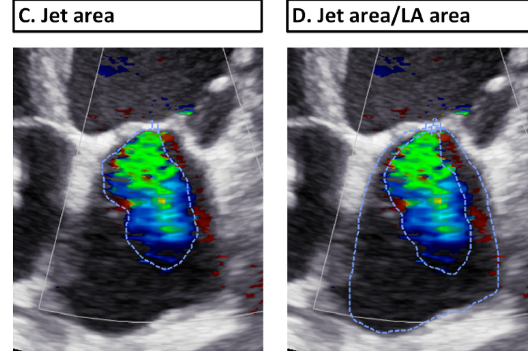
\includegraphics[keepaspectratio]{images/mrjetarea.png}}

\subsubsection{Keuhkovaltimopaine (PAP, PASP)}\label{keuhkovaltimopaine-pap-pasp}

Keuhkovaltimopaineita ei useimmissa guidelineissa käytetä suorana spesifisenä tai edes tukevana kriteerinä mitraalivuodon vaikeusastetta päätellessä, mutta se kuitenkin toimii epäsuorana työkaluna, joka on järkevää mitata monissa tilanteissa (ei siis pelkästään mitraalivuodossa). Keuhkovaltimopaineen nousemista \textgreater50 mmHg käytetään joskus myös indikaationa läpän korjaukselle, jos kyseessä on matalan leikkausriskin potilas ja läpän korjauksen onnistumisen arvioidaan olevan todennäköistä.

Keuhkovaltimopaine nousee johtuen vasemman puolen paineiden nousun takia, jonka takia verta pakkautuu keuhkolaskimoihin ja paineen nouseminen lopulta heijastuu valtimoihinkin. Tällä samalla mekanismilla muutkin vasemman puolen pumppaustoimintaa häiritsevät ongelmat johtavat keuhkovaltimopaineen nousemiseen.

Keuhkovaltimopaineiden epäsuora arviointi tapahtuu tyypilliseen tapaan trikuspidaalivuodon gradientin (TR PG) ja keskuslaskimopaineen (eli oikean eteisen paineen, RAP) mittausten kautta: PASP = TR PG + RAP

RAP siis mitattiin IVC:n paksuuden ja lyttääntymisherkkyyden kautta (kts. IVC-osio)

\subsubsection{Flail leaflet}\label{flail-leaflet}

``Flail leaflet'' eli vapaasti heiluva läppäprolapsi on vaikea mitraaliläpän prolapsin muoto, jossa läpän kärki (ja joskus jopa runko) liikkuvat vapaasti eteiseen ja tämä aiheuttaa yleensä vaikeaa akuuttia vuotoa. Useimmiten taustalla on chordae tendinae -ruptuura (jännerihmarepeämä), mutta joskus jopa papillaarilihasruptuura. Jännerihmojen repeämisen taustalla voi olla mm. läpän myksomatoottinen rappeuma (usein mitraaliläpän prolapsin yhteydessä), infektiivinen endokardiitti tai reumakuumeen komplikaatio. Endokardiitti voi myös suoraan vaurioittaa läppärakenteita ja siten aiheuttaa ei-iskeemistä akuuttia vuotoa. Papillaarilihasruptuura on taas tyypillisesti iskeeminen etiologialtaan ja syntyy useimmiten n.~3-5pv infarktin jälkeen.

Useimmiten flail leaflet on posteriorinen purje ja vielä tarkemmin P2 johtuen sen korkeasta mekaanisesta stressistä ja jännerihmayhteyksistä.

Kannattaa mitata mahdollisuuksien mukaan flail gap (vaikuttaa leikkauksen aiheellisuuteen).

\pandocbounded{\includegraphics[keepaspectratio]{images/flailplax.gif}}
\pandocbounded{\includegraphics[keepaspectratio]{images/flaila4c.gif}}
\pandocbounded{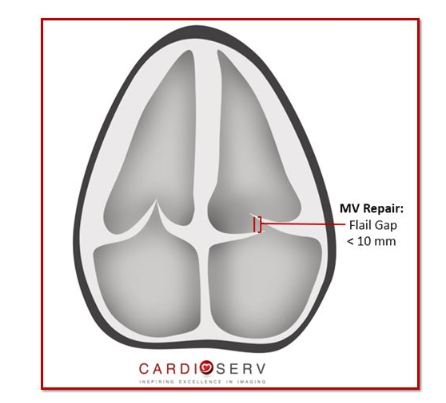
\includegraphics[keepaspectratio]{images/flailgap.png}}

\subsection{Vaikeusasteet}\label{vaikeusasteet}

Mitraalivuodon gradeerauksessa nykyään yleisin luokittelu on lievään, keskivaikeaan ja vaikeaan. Joskus graduksen voi myös ilmoittaa numeerisella skaalalla gr I - IV, jossa gr III voi olla joko keskivaikea tai vaikea.

ASE:n ja ESC:n guidelinet ovat pääasiassa samanlaiset ja ne perustuvat niin kvalitatiiviset, semikvantitatiiviset kuin kvantitatiiviset parametrit integroivaan lähestymistapaan. Tärkeimmät kvantitatiiviset mitat ovat EROA, vuodon tilavuus (RVol) ja vuotofraktio (RF). Ennen niidenkin laskemista tai mittausarvoja kerätessä voi jo nopean algoritmin perusteella sulkea pois tai todeta lievän tai vaikean vuodon. Kannattaakin mitraalivuotoa arvioidessaan seurata tyypillistä järjestystä tutkimuksessaan:

\pandocbounded{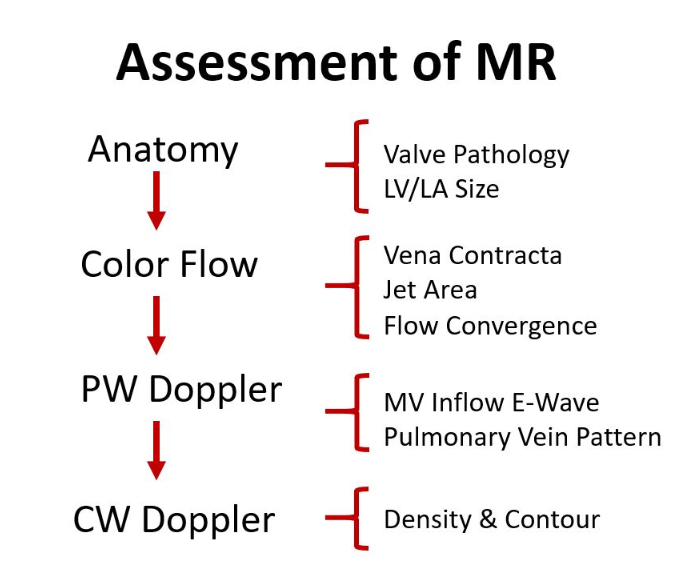
\includegraphics[keepaspectratio]{images/mrassessment.png}}

Tätä ``algoritmia'' seuraten tulee mitattua tärkeimmät asiat ja alla kuvassa olevien kriteerien mukaan voi poissulkea tai todeta lievän tai vaikean vuodon. Jos kriteerit ei täyty eli tulokset ovat varmasti lievän ja varmasti vaikean välissä, niin kvantitatiivisilla mittauksilla saa tarkemman arvion vaikeusasteesta. Kvantitatiiviset mittaukset on kuitenkin hyvä muutenkin ottaa aina mahdollisuuksien mukaan.

\pandocbounded{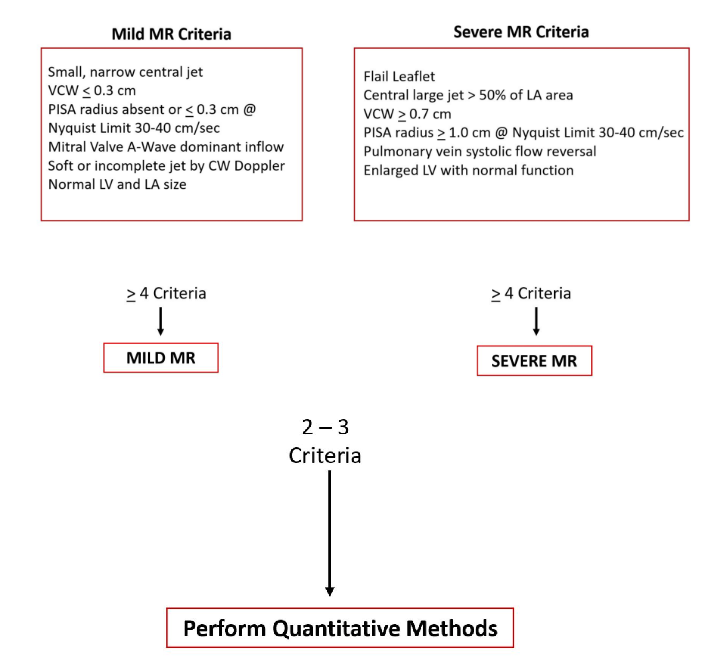
\includegraphics[keepaspectratio]{images/mrcriteria.png}}

Kvantitatiivisista metodeista saa siis aikaisemmin mainittuun tapaan arvot EROA, RVol ja RF. Monesti voi tehdä vaikeusasteen lausunnon jo pelkästään näiden perusteella. Simppelissä lähestymistavassa jako voi olla pelkästään lievään, keskivaikeaan ja vaikeaan, mutta tarkemmassa gr I - IV -jaottelussa gr III voi sisältää myös vaikean vuodon. Jos siis on 3 spesifistä keskivaikean vuodon rajojen yläpäähän sijoittuvaa tulosta (EROA 0.3-0.39, RVol 45-59 ml ja RF 40-49\%), niin vuoto voi olla gr III (severe) ja jos taas tulokset ovat enemmänkin rajojen alkupäässä niin gradus on III (moderate). Nämä ovat myös vaikean vuodon kriteerit sekundaariselle (toiminnalliselle) vuodolle, koska mittaukset usein aliarvioivat sekundaarisen vuodon vaikeusastetta.

\pandocbounded{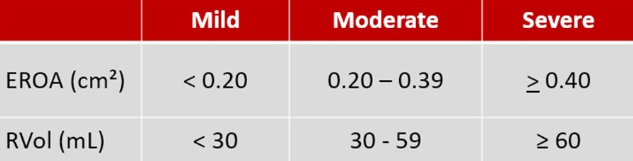
\includegraphics[keepaspectratio]{images/mrseveritysimple.png}}
\pandocbounded{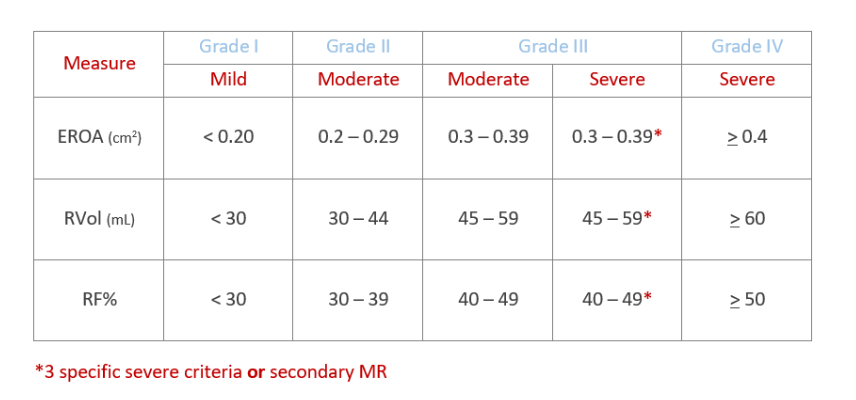
\includegraphics[keepaspectratio]{images/mrgrades.png}}
\pandocbounded{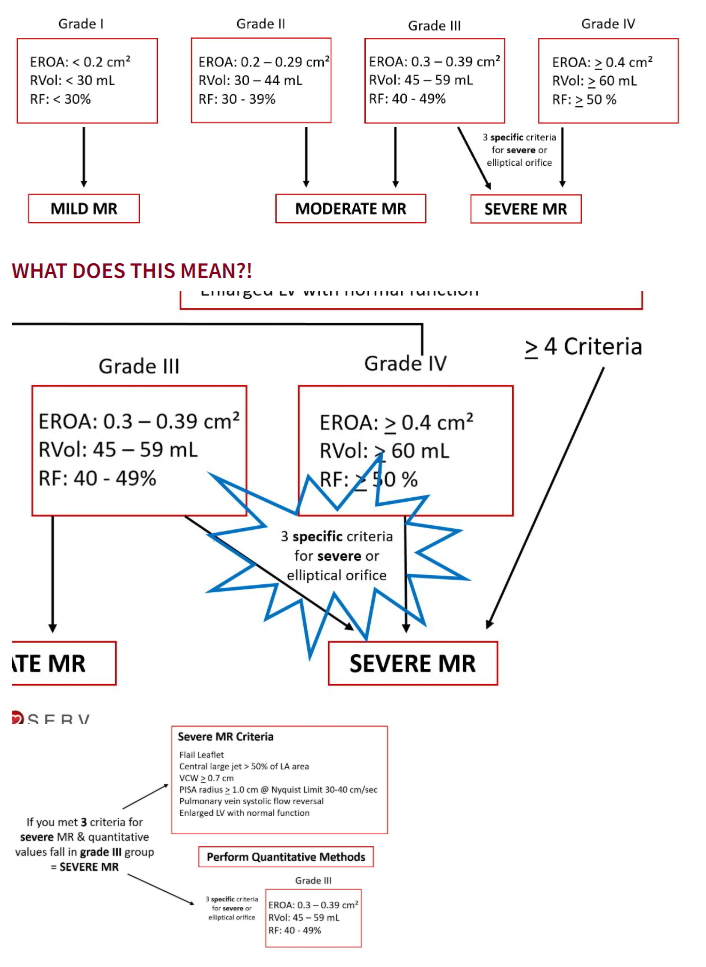
\includegraphics[keepaspectratio]{images/graduswhat.png}}

Tässä vielä kokonaisuudessaan ASE:n algoritmi:

\pandocbounded{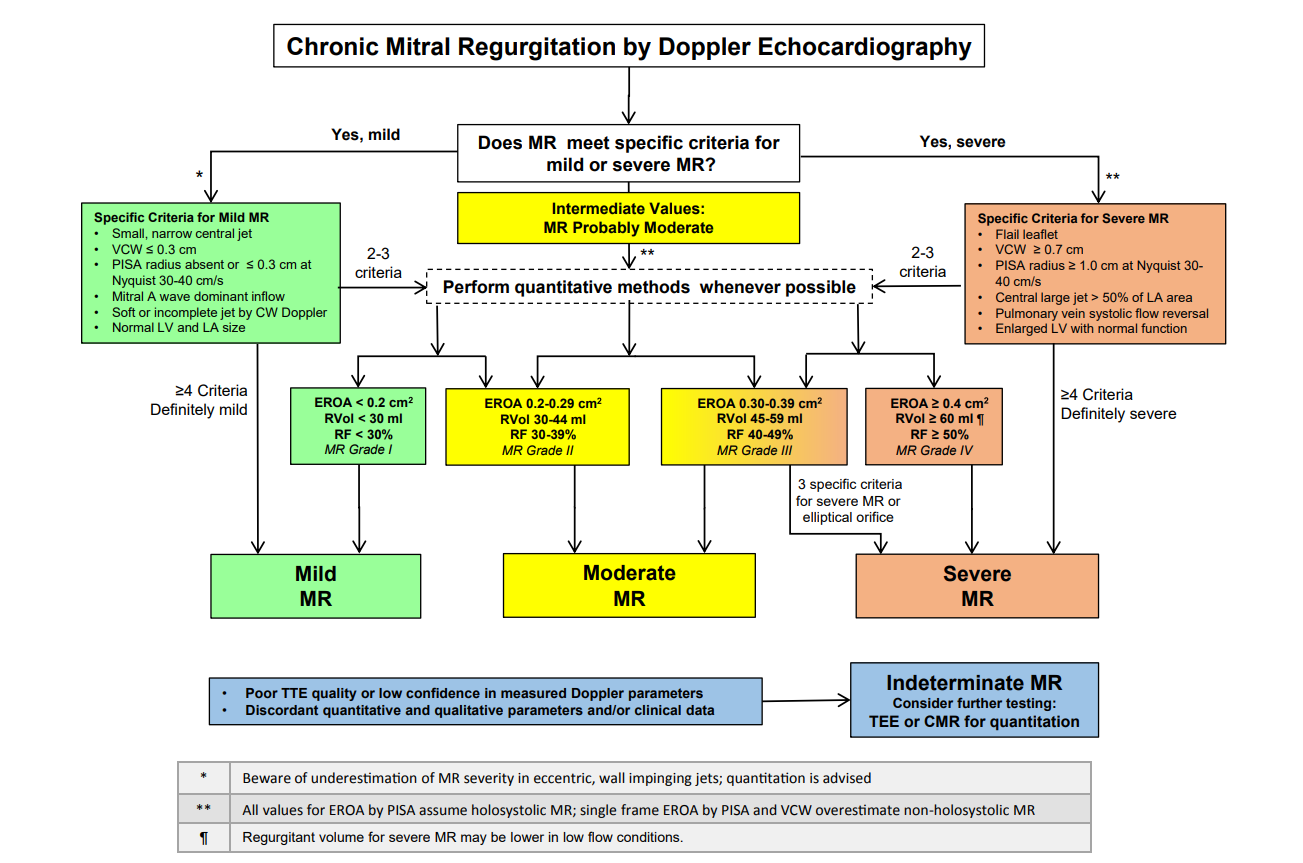
\includegraphics[keepaspectratio]{images/mitralregurgitationgrade.png}}

\section{Muuta huomioitavaa}\label{muuta-huomioitavaa}

Vaikeusasteen arvioinnissa on monia huomioitavia asioita, jotka voivat ohjata tutkijan harhaan. Tässä on pari tärkeintä jo aikaisemmin mainittujen lisäksi.

\subsection{Vuodon kesto}\label{vuodon-kesto}

Mitraalivuodon kesto on tärkeää ottaa huomioon. Jos MR rajoittuu myöhäissystoleen (kuten yleensä mitraaliläppäprolapsissa (MVP)) tai aikaissystoleen (esim. kammiodyssynkronia), niin vuoto ei ole yleensä vaikea-asteinen. Usein kuitenkin näissä tilanteissa tulee tehtyä virhearvio, jos pohjustaa arvion vain yksittäisiin väridopplerin freeze frame -mittauksiin, kuten vuodon kaulaan tai PISA:an.

\pandocbounded{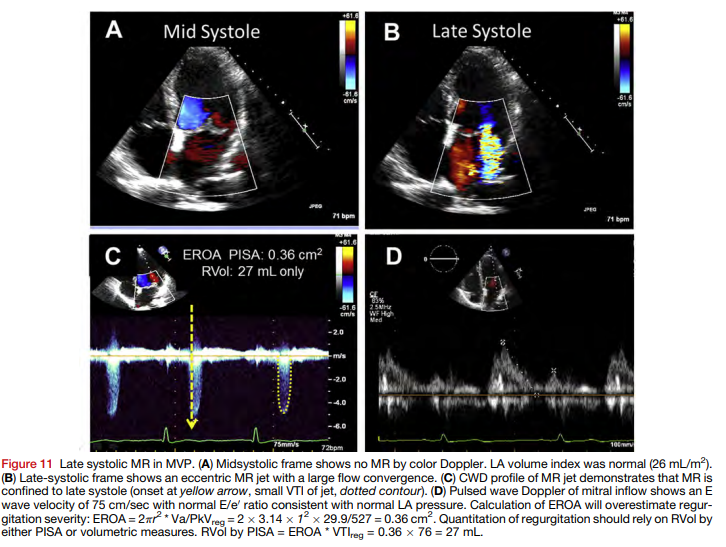
\includegraphics[keepaspectratio]{images/mvpmroverestimation.png}}
\#\#\# Paineiden vaikutus

Hemodynaamiset muutokset, varsinkin verenpaine, voivat vaikuttaa merkittävästi MR:n vaikeusasteen arvioon. Korkea verenpaine tarkoittaa sitä, että vasemman kammion paineiden on pakko nousta systolessa myös korkealle (esim. jos systolinen verenpaine on 170 mmHg, niin vasemman kammion on pakko supistua niin kovaa, että sen sisäinen paine nousee vähintään arvoon 170mmHg (jotta aorttaläppä edes aukeaisi)). Tästä johtuen paine-ero kammion ja eteisen välillä on suuri ja koska paine-ero puristaa verta vuotoaukon läpi suurella voimalla, on vuotovirtaus todella nopea.

Nopeat virtaukset (esim. \textgreater6 cm/s) voivat näyttää merkittävänkin suurilta väridopplerissa, vaikka EROA tai RVol olisivatkin pienet. Tällainen tilanne on siis usein esim. hypertensiossa, vaikeassa aorttastenoosissa tai merkittävässä LVOT-obstruktiossa. Hypotensiossa taas vuotosuihku voi näyttää suhteellisen pieneltä, vaikka vuoto olisikin todellisuudessa vaikea.

Älä siis tee päätöksiä vuodon vaikeudesta pelkästään silmämääräisen vuotosuihkun suuruuden (tai edes vuotosuihkun ja eteisen pinta-alojen suhteen) tai CW-dopplerin virtausnopeuksien perusteella!

\pandocbounded{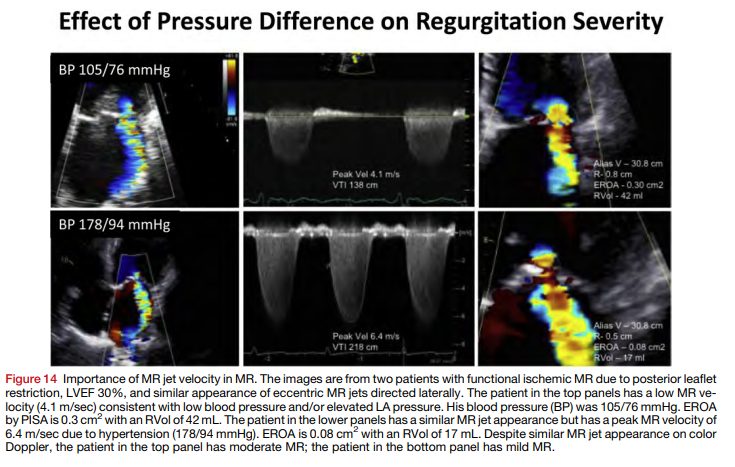
\includegraphics[keepaspectratio]{images/mrpressures.png}}

\section{Hoito}\label{hoito}

Nykyiset hoitosuositukset jakavat mitraalivuodon hoidon kahteen eri polkuun sen mukaan, onko vika rakenteellinen itse läpässä (primaarinen) vai onko vika toiminnallinen (sekundaarinen). Tässä on molempien hoitolinjojen algoritmit:

\pandocbounded{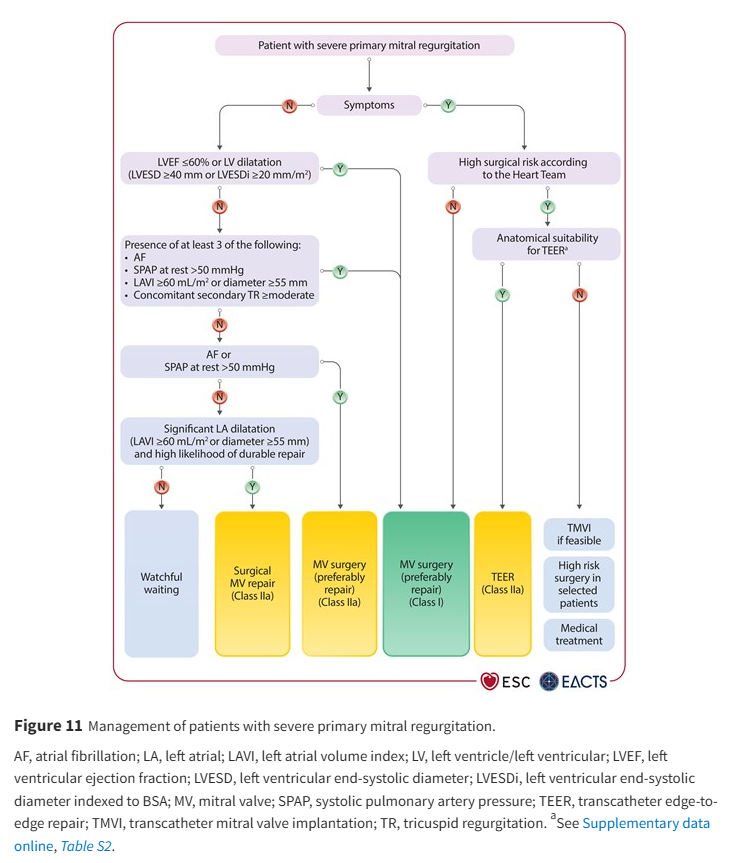
\includegraphics[keepaspectratio]{images/primarymr.png}}
\pandocbounded{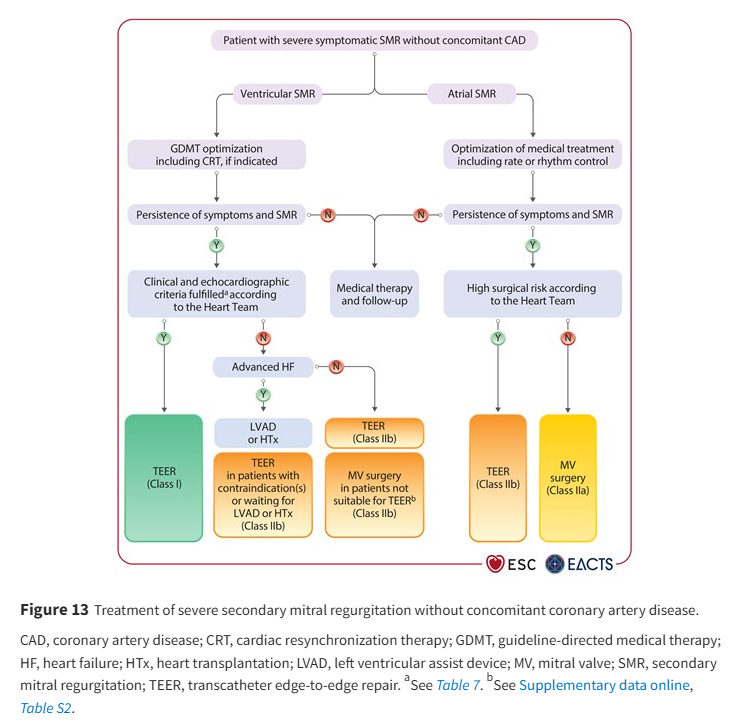
\includegraphics[keepaspectratio]{images/secondarymr.png}}

\subsection{Primaarisen mitraalivuodon operatiivisen hoidon indikaatiot}\label{primaarisen-mitraalivuodon-operatiivisen-hoidon-indikaatiot}

Primaarisessa vuodossa ongelma on rakenteellinen, joten hoitokin keskittyy pääasiassa rakenteelliseen korjaukseen. Lääkkeillä ei voida korjata perforoitunutta läppää tai revenneitä kordia, vaan ne auttavat ainoastaan oireiden (kuten nesteen kertymisen) hallinnassa leikkausta odotellessa.

Kirurginen hoito on yleensä aiheellista \emph{vaikeassa} mitraalivuodossa oireiden ilmestyessä. Oireettomillakin potilailla leikkaus on yleensä aiheellinen, jos LVEF laskee alle 60\%:iin tai kammio dilatoituu (LVESD ≥ 40mm tai LVESDi ≥ 20 mm/m2; LVESDi on siis Left Ventricular End-Systolic Dimension Indexed to body surface area).

Mitraalivuodon gradeerauksen lisäksi tulisi myös muistaa arvioida myös aina mahdollisuuksien mukaan mm. ejektiofraktio, lokeroiden (LA ja LV) mitat ja keuhkovaltimopaineet mahdollisimman hyvin, koska niitä käytetään leikkauksen aiheellisuutta arvioitaessa. Oireettomillakin potilailla leikkaus voi hyvinkin olla kannattavaa, jos todetaan huonon prognoosin merkkejä, joita ovat esimerkiksi kohonneet keuhkovaltimopaineet (\textgreater50 mmHg levossa), vähintään keskivaikea sekundaarinen trikuspidaalivuoto, eteisvärinäjaksot ja vasemman eteisen huomattava laajeneminen (LAVi ≥ 60ml tai läpimitta ≥ 55mm).

\pandocbounded{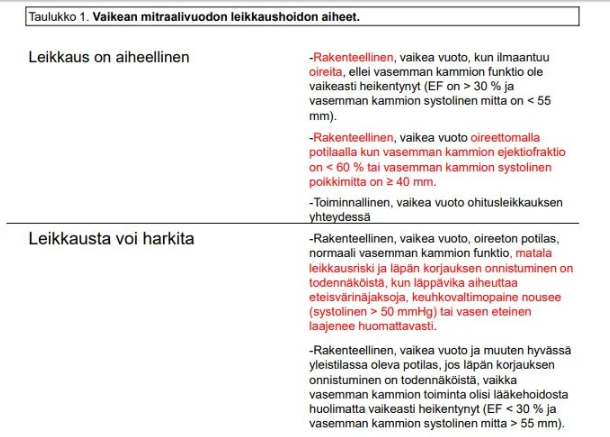
\includegraphics[keepaspectratio]{images/mitraalivuodonleikkausaiheetdia.png}}
\pandocbounded{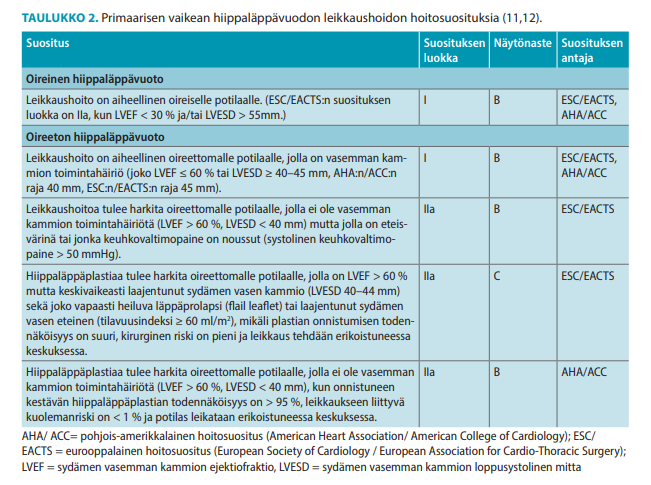
\includegraphics[keepaspectratio]{images/mrleikkausindikaatiot.png}}

\subsection{Sekundaarinen mitraalivuoto}\label{sekundaarinen-mitraalivuoto}

Sekundaarisessa vuodossa itse läppä on terve, mutta vasen kammio tai eteinen on laajentunut ja vetää läppäpurjeet erilleen (kuten aiemmin käsitellyt Carpentier I ja IIIb -luokat). Ongelma on sydänlihaksessa, joten hoidetaan ensin lihasta. Kirurgiaan suhtaudutaan paljon pidättyvämmin, koska pelkän läpän korjaaminen ei useinkaan paranna huonokuntoisen sydänlihaksen ennustetta.

Tämän takia sekundaarisen mitraalivuodon hoito perustuu ensisijaisesti optimaaliseen sydämen vajaatoiminnan ennusteelliseen lääkehoitoon (ACEi/ATRi (/ARNI) + beetasalpaaja + MRA + SGLT2i) ja tarvittaessa diureetteihin. Mahdollisesti voidaan myös käyttää iskeemisissä ongelmissa tietysti revaskulaarisaatiohoitojakin. Jos vajaatoimintatahdistinhoidon (CRT) kriteerit (optimaalisesta lääkehoidosta huolimatta sinusrytmissä olevalla potilaalla on oireita (NYHA II-IV), ja EF on ≤ 35 \% ja EKG:ssä LBBB-konfiguraatio, jonka QRS-kesto on vähintään 150 ms) täyttyvät niin sekin tietysti voi olla indikoitua.

Jos potilas on edelleen oireinen raskaasta lääkehoidosta huolimatta ja vuoto on vaikea, niin voidaan harkita toimenpiteellistä hoitoa, joka voi tilanteesta riippuen olla perkutaaninen hoito (MitraClip; etenevissä määrin) tai kirurgia (vieläkin ensisijaisempi atriaalisessa vuodossa eli carpentier I-tyypin vuodossa). Leikkaushoito tulee ensisijaisesti kyseeseen, jos avosydänleikkaukselle on muu aihe (esim. ohitusleikkaus sepelvaltimotaudin vuoksi), ja melko harvoin itsenäisenä toimenpiteenä (on vain niukasti näyttöä siitä, että kroonisen toiminnallisen hiippaläppävuodon leikkaushoidolla voitaisiin parantaa potilaiden ennustetta tai edes oireisuutta pitkän ajan seurannassa).

\begin{center}\rule{0.5\linewidth}{0.5pt}\end{center}

LVEF:n arvio on tärkeää niin kirurgian kuin muiden toimenpiteiden aiheellisuutta ja vasta-aiheellisuutta mietittäessä (niin primaarisessa kuin sekundaarisessakin vuodossa). Jos LVEF tippuu alle 20-30\%:iin (20-30\%-väli on varsinkin mitraclipissä vielä ok; optimaalinen on 20-50\%), niin sydänlihas on usein jo niin sanotusti ``loppuunpalanut'' ja pelkkä mitraaliläpän vuodon korjaaminen klipsillä tai leikkauksella ei yleensä enää auta potilasta, koska itse pumppu on liian heikko. Leikkausriski on myös merkittävän korkea. Kuitenkin jos potilas on muuten hyvässä yleistilassa ja läpän korjaamisen ajatellaan olevan todennäköisesti mahdollista, niin toimenpiteellisiä hoitoja voidaan harkita jos lääkkeet eivät riitä.

\subsection{Leikkaus vs perkutaaninen klipsaus}\label{leikkaus-vs-perkutaaninen-klipsaus}

Läppäplastiaa ja tekoläppäleikkausta vertailevia satunnaistettuja tutkimuksia ei ole, mutta takautuvissa vertailevissa analyyseissa ennuste on hiippaläppäplastian jälkeen ollut toistetusti parempi kuin tekoläppäleikkauksen jälkeen. Sekä eurooppalainen että pohjoisamerikkalainen hoitosuositus suosittelevatkin vahvasti, että ensisijaisesti tulee pyrkiä hiippaläppäplastiaan. Plastian etuja tekoläppäleikkaukseen verrattuna ovat pienempi leikkauskuolleisuus ja parempi pitkäaikaisennuste useissa satunnaistamattomissa tutkimuksissa, tekoläpän haittojen kuten mekaaniseen tekoläppään liittyvän pysyvän antikoagulaation ja kudostekoläpän rakenteellisen vaurioitumisen välttäminen sekä seurannassa vähäisempi endokardiitin, tromboembolian ja vakavan verenvuodon riski. Leikkaus tehdään yleensä sternotomiateitse sydän-keuhkokonetta käyttäen.

Suuren riskin (riskilaskureita on monia; esim. STS Adult Cardiac Surgery Database tai EuroSCORE II) takia leikkaushoito ei ole aina mahdollinen, ja toiminnallisen vuodon yhteydessä leikkaushoidon hyötykin on epävarma. Perkutaanisia katetritekniikoita ja muita vaihtoehtoja perinteiselle mitraalivuodon avosydänleikkaukselle on täten kehitetty aktiivisesti. Mitraalivuodon hoidossa laajimmin käytössä oleva perkutaaninen korjaustekniikka on klipsihoito MitraClip-tekniikalla (yllä olevissa algoritmeissa lyhenne on TEER eli Transcatheter Edge-to-Edge Repair), jota on Suomessa käytetty vaikean hiippaläppävuodon hoitoon vuodesta 2011 lähtien.

Menetelmässä viedään MitraClip-laite yleisanestesiassa reisilaskimopunktion kautta oikeaan eteiseen, josta vasempaan eteiseen päästään transseptaalisen punktion kautta (yleensä fossa ovaliksen kohdalta, koska se on valmiiksi ohut). Laite viedään mitraaliläpän alueelle ja läpän etu- ja takapurjeen reunat kiinnitetään toisiinsa keskiosistaan klipsillä. Syntyy tupla-aukkoinen mitraaliläppä (double orifice), joka sulkeutuu paremmin kuin ennen toimenpidettä. Toimenpide tehdään TEE-ohjauksessa (myös fluoroskopia samalla katetrien ja ohjainlankojen kanssa).

Hoitomuoto sopii parhaiten toiminnallisen vuodon hoitoon. Jos potilaan leikkausriski arvioidaan hyvin suureksi, voidaan rakenteellisissakin vuodoissa tehdä katetritoimenpide. Hyvällä potilasvalinnalla \textgreater90\%:a potilaista hyötyy toimenpiteestä ja komplikaatiot ovat harvinaisia; kotiutuminen voi yleensä tapahtua jo seuraavana päivänä. Onnistunut potilasvalinta edellyttää huolellista hiippaläpän rakenteen ja toiminnan tutkimista ruokatorven kautta tehtävällä kaikukuvauksella (TEE). Tästä huolimatta katetrikorjaus ei aina onnistu, erityisesti silloin, kun hiippaläpän vuodon mekanismina on rakenteellinen läppävika. Toiminnallisen hiippaläppävuodon Mitracliphoidosta saattaa olla ennusteellista hyötyä, mutta näyttö on osin ristiriitaista ja pidemmän ajan seurantatuloksia tarvitaan.

Hiippaläpän toiminnallisen vuodon klipsihoitoa käytetään Suomessa vielä liian vähän. Vuonna 2022 näitä toimenpiteitä tehtiin Suomessa 35 kpl. Kyseessä on siis aika harvinainen toimenpide. Liian usein potilaat lähetetään hoitoarvioon vasta, kun vasemman kammion toiminta on jo vaikeasti huonontunut. Tällöin hoitotulos ei välttämättä ole paras mahdollinen.

\pandocbounded{
\includegraphics[keepaspectratio]{images/mitraclip.gif}}
\pandocbounded{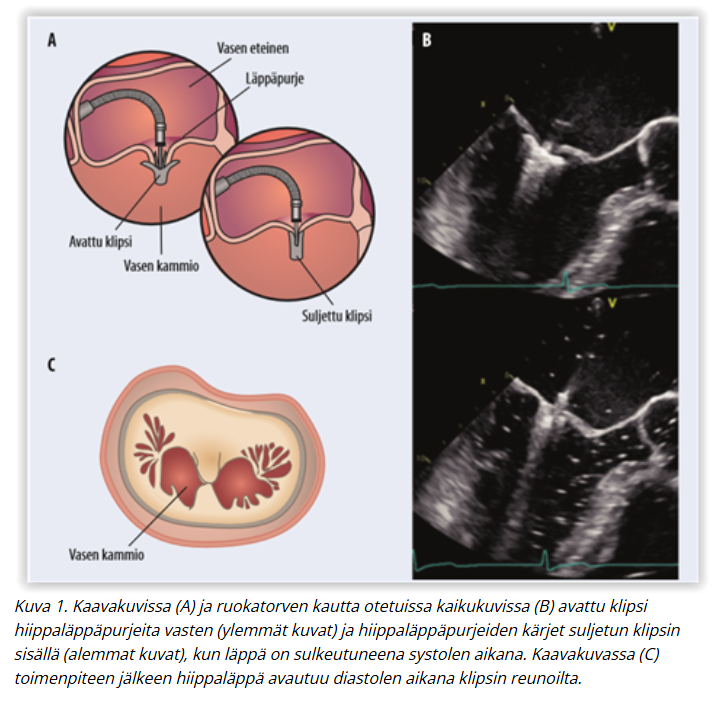
\includegraphics[keepaspectratio]{images/mitraclip.png}}

\chapter{Dyssynkronia ja paikalliset liikehäiriöt}\label{dyssynkronia-ja-paikalliset-liikehuxe4iriuxf6t}

\chapter{Perikardiumtila}\label{perikardiumtila}

\chapter{Sydämensisäiset massat}\label{Massat}

\chapter{Keuhkot}\label{keuhkot}

\chapter{Askites}\label{askites}

Alla olevat ohjeet ja kuvat ovat pitkälti \href{https://youtu.be/dUaCWK3qoHM?si=knKxswGwp-eyTIW0}{tältä todella hyvältä Jason Williamsin videolta} kerättyjä.

\section{Anturi}\label{anturi}

\section{Hyvän taskun löytäminen}\label{Tasku}

Jotta löytää mahdollisimman hyvän nestekertymän punktoitavaksi, niin kannattaa aloittaa ihan fyysisesti asennoimalla potilas niin, että nestetasku tyypillisissä pistokohdissa on maksimaalisen suuri. Koska punktio tehdään yleensä alaneljänneksiltä (ilman ultraääntä tyypillinen pistokohta on yleensä n.~3cm päähän päin ja 3cm mediaalisesti spina iliaca anterior superiorista), niin kannattaa siis aloittaa nostamalla sängyn päätyä, jotta painovoima saa vedettyä nestettä vatsaontelon alaosiin helpommin. Tämän jälkeen tulee skannata molemmat alaneljännekset kahdessa tasossa, löytää suurin nestetasku ja hieman pyöräyttää potilasta sille puolelle.

Turvallisen kertymän tulisi olla n.~3cm x 3cm x 3cm. Jos kertymä on tätä pienempi, niin parasenteesi tulisi vähintäänkin tehdä jatkuvan ultraäänivisualisaation aikana (dynaaminen tekniikka).

\pandocbounded{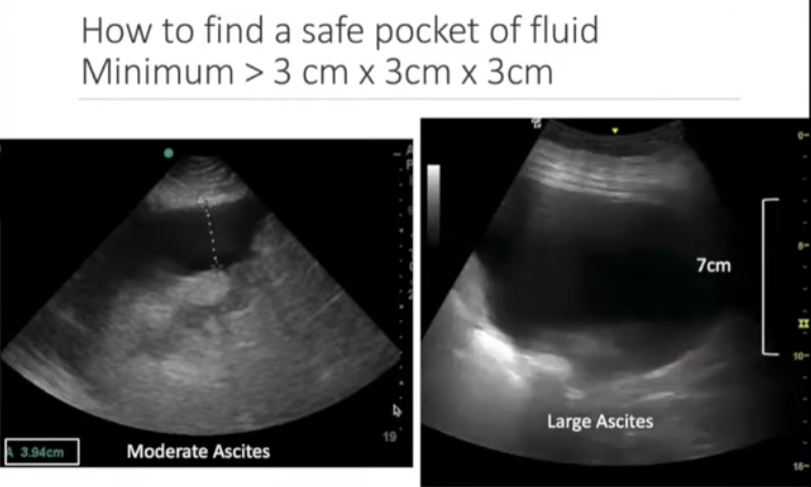
\includegraphics[keepaspectratio]{images/askiteshyvätasku.png}}

\subsection{Skannaaminen kahdessa tasossa}\label{skannaaminen-kahdessa-tasossa}

Vaikka yhdellä anturin orientaatiolla löytäisi hyvän nestekertymän, niin tulisi skannata myös vähintäänkin kohtisuora orientaatio, jotta voi nähdä läheisiä rakenteita paremmin. Erityisesti tulisi siis etsiä pitkittäisleikkeestä (anturin orientaatio potilaan pitkittäisakselin (jalat-pää) mukaisesti) ipsilateraalinen maksa tai perna (ja munuainen). Ne voivat olla yllättävän lähellä ja niiden lähelle tehtävää punktiota tulisi mahdollisuuksien mukaan välttää (probea voi siis liu'uttaa jalkoihin päin niistä poispäin).

\pandocbounded{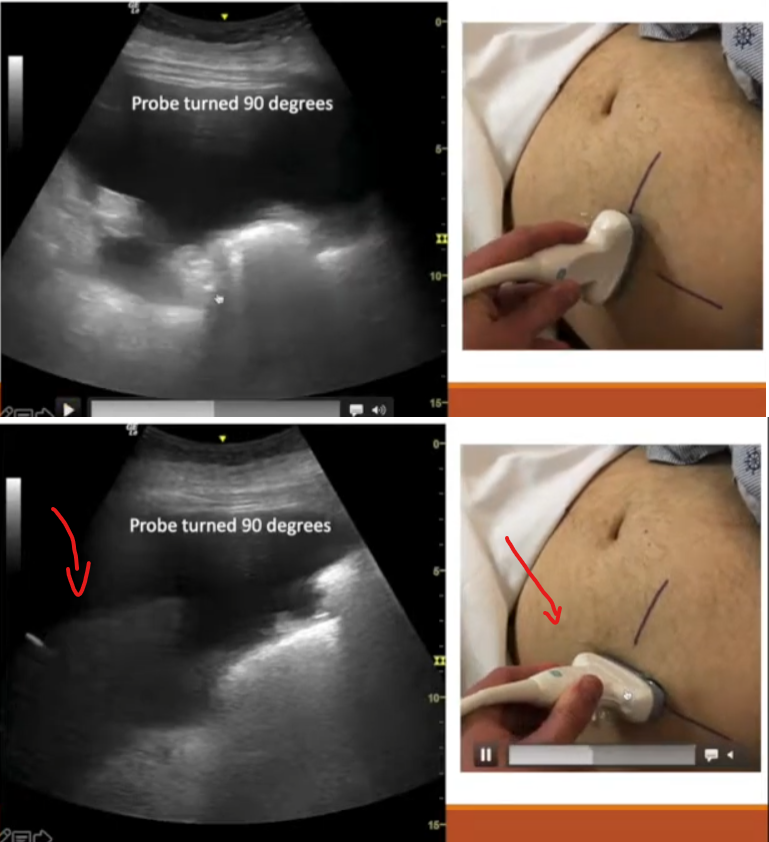
\includegraphics[keepaspectratio]{images/2maksa.png}}

\section{Miten vähentää verenvuotoriskiä?}\label{miten-vuxe4hentuxe4uxe4-verenvuotoriskiuxe4}

Verenvuoto on askitespunktion yleisin komplikaatio, mutta toimenpidettä edeltävällä ultraäänitutkimuksella saa minimoitua tämän riskin todella matalaksi.

Yleinen ohje ilman ultraääntäkin on se, että punktiossa tulisi välttää suorien vastalihasten faskiatuppea (rectus sheath), koska siinä kulkee epigastriset valtimot ja laskimot. Yleisimmin vaurioituva valtimo on juuri a. epigastrica inferior. Tyypillisimmin se tulee vältettyä jo ihan visuaalisesti arvioimalla rectustupen alue ja pistämällä siitä lateraalisesti (on myös muita pistolokaatioita, mutta lateraalinen on yleisin).

Usein kuitenkin askiteksen venyttäessä kudoksia, on vaikeaa erottaa, missä vatsalihakset oikeasti kulkevat. Varsinkin näissä tapauksissa on ultraääniselvittelyistä hyötyä.

\pandocbounded{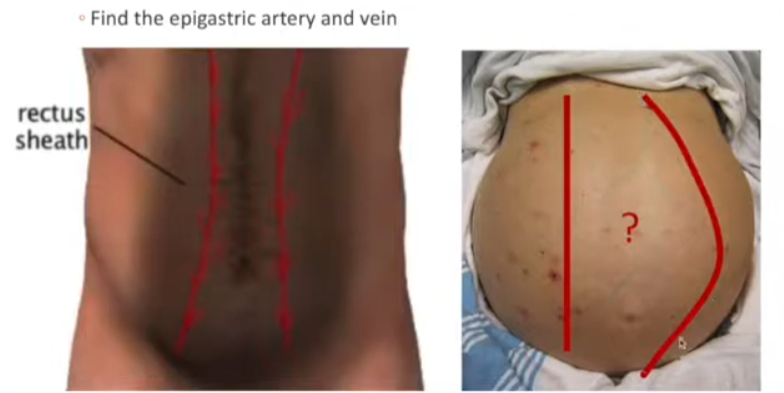
\includegraphics[keepaspectratio]{images/findtheepigastricarteryandvein.png}}
\pandocbounded{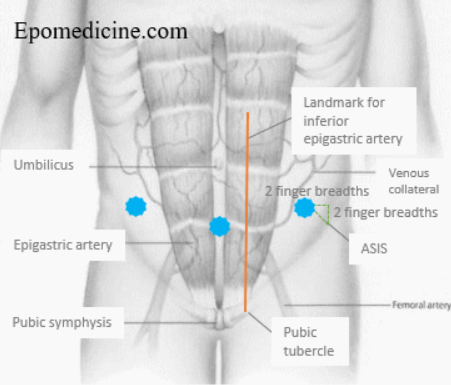
\includegraphics[keepaspectratio]{images/epomedicine.png}}

\begin{center}\rule{0.5\linewidth}{0.5pt}\end{center}

Merkittävät verisuonet saa esiin skannaamalla toimenpidealuetta neljässä suunnassa ja arvioimalla subkutaanisia faskiatasoja. Paras anturi tämän suhteen on lineaarinen anturi.

Suonia kannattaa skannata neljässä tasossa sekä myös anturia vähän näissä tasoissa tiltaten, jotta nostaa todennäköisyyttä löytää kaikki merkittävät suonet. Suonet tulevat parhaiten näkyviin, kun anturi on kohtisuorassa niiden suhteen. Suonet kulkevat vatsaontelon seinämässä eri kulmissa ja täten eri kulmissa skannaaminen on hyödyllistä. Myös doppleria kannattaa käyttää näissä skannaustasoissa, jotta voi nähdä muuten heikosti visualisoituvat suonet (doppler on tässä jokseenkin heikko herkkyydeltään, mutta korkea tarkkuudeltaan).

Merkittävät suonet yleensä tunnistaa siitä, että näkee kaksi suonta yhdessä; nämä ovat käytännössä aina valtimo ja laskimo. Tällaista ``double vessel sign''-kohtaa kannattaa välttää.

\pandocbounded{\includegraphics[keepaspectratio]{images/4planes.gif}}
\pandocbounded{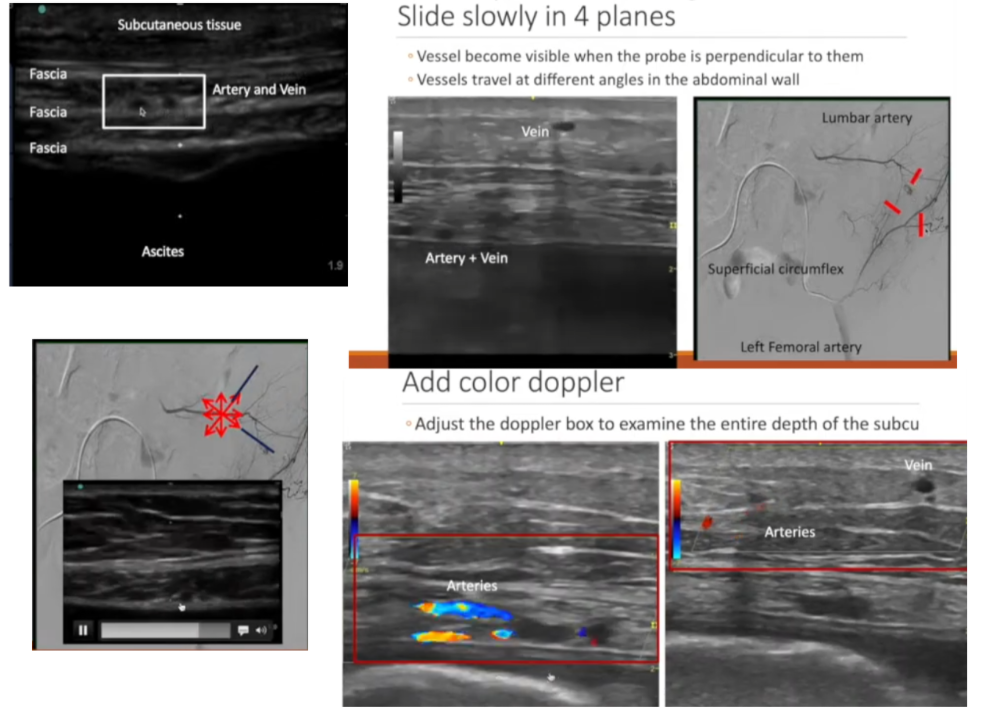
\includegraphics[keepaspectratio]{images/vesselfindingcompilation.png}}

\section{Pistoreitin suunnittelu}\label{Pistoreitti}

Viimeistään toimenpidettä edeltävästi kannattaa anturin kulmaa muuttamalla vielä selvitellä nestetaskun muotoa ja kokoa. Kun löytää sopivan kulman, jossa tasku on suurin ja reitti näyttää turvallisimmalta, niin kannattaa painaa mieleen anturin senhetkinen kulma ja myös pistää neula läpi tässä kulmassa.

Kannattaa myös katsoa, kuinka paksu vatsanseinämä on suunnitellussa pistokohdassa: tämä auttaa itse toimenpiteessä paljon, kun jo etukäteen tietää, kuinka pitkä matka lävistettävään peritoneumiin on. Vatsanseinämän ja lisäksi askitesnestekertymän paksuuden tietäminen auttaa myös sen arviossa, kuinka syvälle katetri viedään (sitä ei tulisi vielä suoleen saakka, koska suoli voi tukkia imukanavia ja sitä kautta estää dreneerausta).

\pandocbounded{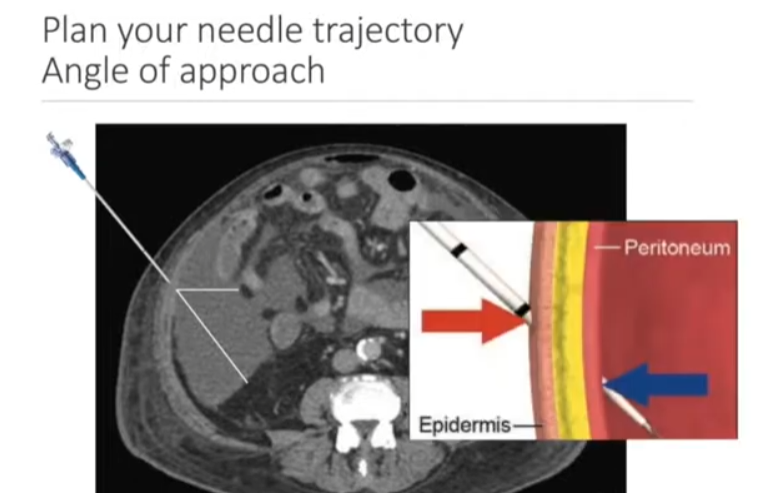
\includegraphics[keepaspectratio]{images/angleofapproach.png}}
\pandocbounded{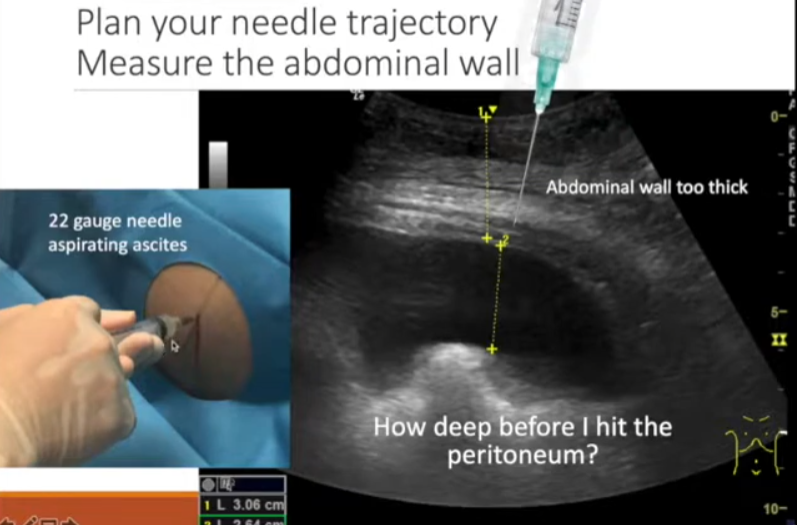
\includegraphics[keepaspectratio]{images/abdominalwallthickness.png}}

\chapter{Maksa}\label{maksa}

\chapter{Vatsa-aortta}\label{vatsa-aortta}

\chapter{Rakko}\label{rakko}

\bibliography{book.bib,packages.bib}

\end{document}
